%%%%%%%%%%%%%%%%%%%%%%%%%%%%%%%%%%%%%%%%%%%%%%%%%%%%%%%%%%%%%%%%%%%%%%
% Overleaf (WriteLaTeX) Example: Molecular Chemistry Presentation
%
% Source: http://www.overleaf.com
%
% In these slides we show how Overleaf can be used with standard 
% chemistry packages to easily create professional presentations.
% 
% Feel free to distribute this example, but please keep the referral
% to overleaf.com
% 
%%%%%%%%%%%%%%%%%%%%%%%%%%%%%%%%%%%%%%%%%%%%%%%%%%%%%%%%%%%%%%%%%%%%%%

\documentclass[xcolor={dvipsnames}]{beamer}

\mode<presentation>
{
  \usetheme{Madrid}       % or try default, Darmstadt, Warsaw, ...
  \usecolortheme{default} % or try albatross, beaver, crane, ...
  \usefonttheme{default}    % or try default, structurebold, ...
  \setbeamertemplate{navigation symbols}{}
  \setbeamertemplate{caption}[numbered]
} 

\usepackage[english]{babel}
\usepackage[utf8x]{inputenc}
\usepackage{graphicx}
\usepackage{hyperref}
  \hypersetup{colorlinks=true}
  \hypersetup{urlcolor=blue}
  \hypersetup{linkcolor = .}
\usepackage{xcolor}
\usepackage{siunitx}
  \sisetup{separate-uncertainty = true}
\DeclareSIUnit\barn{b}
\usepackage{physics}
\usepackage[font=small,labelfont=bf]{caption}
\usepackage{subcaption}
\usepackage[en-GB]{datetime2}
\usepackage{overpic}
\usepackage{feynmp}
\DeclareGraphicsRule{*}{mps}{*}{}
\usepackage{scalerel}
\newcommand{\mylbrace}[2]{\vspace{#2pt}\hspace{6pt}\scaleleftright[\dimexpr5pt+#1\dimexpr0.06pt]{\lbrace}{\rule[\dimexpr2pt-#1\dimexpr0.5pt]{-4pt}{#1pt}}{.}}
\newcommand{\myrbrace}[2]{\vspace{#2pt}\scaleleftright[\dimexpr5pt+#1\dimexpr0.06pt]{.}{\rule[\dimexpr2pt-#1\dimexpr0.5pt]{-4pt}{#1pt}}{\rbrace}\hspace{6pt}}

% Trim in percent
\usepackage{adjustbox}

% No "Figure" prefix
\setbeamertemplate{caption}{\raggedright\insertcaption\par}

% Nice decay amplitude diagrams
\usepackage{amsmath,amssymb,tikz-cd}

% Strike out text
\usepackage[normalem]{ulem}

% For figures with text overlay
\usepackage{overpic}

% Arrows
\usepackage{tikz}
\newcommand{\tikzmark}[1]{\tikz[remember picture] \node[coordinate] (#1) {#1};}

% Colourbox with line breaks
\newcommand{\cbox}[2][lime!20]{%
  \colorbox{#1}{\parbox{\dimexpr\linewidth-2\fboxsep}{\strut #2\strut}}%
}

% Vector arrows
\usepackage[pdftex]{pict2e}

% Checkmark symbol
\def\checkmark{\tikz\fill[scale=0.4](0,.35) -- (.25,0) -- (1,.7) -- (.25,.15) -- cycle;} 

% Here's where the presentation starts, with the info for the title slide
\title[Analysis approval]{Model-independent measurement of \texorpdfstring{$\gamma$}{gamma} using \texorpdfstring{$B^\pm\to[h^+h^-\pi^+\pi^-]_Dh^\pm$}{B2DhD2hhpipi} decays}

\author[Martin Tat]{Sneha Malde \inst{1}, Jonas Rademacker \inst{2}, \textbf{Martin Tat}\inst{1,4}, Ben Westhenry \inst{2}, Mark Whitehead \inst{3}, Guy Wilkinson \inst{1}}
\institute[University of Oxford]{\tiny \inst{1} University of Oxford, \inst{2} University of Bristol, \inst{3} University of Glasgow, \inst{4} Heidelberg University}
\date{5th September 2024}

\titlegraphic{
\includegraphics[height = 1.5cm]{lhcb.jpg}\hspace{0.0cm}~%
              
\includegraphics[height = 1.5cm]{HeidelbergLogo.pdf}\hspace{0.0cm}~%
              
\includegraphics[height = 1.5cm]{OxfordLogo.pdf}\hspace{0.0cm}~%
              
\includegraphics[height = 1.5cm]{Bristol_logo.jpg}}

\begin{document}

\begin{frame}
  \titlepage
\end{frame}

% These three lines create an automatically generated table of contents.
\begin{frame}{Outline}
  \tableofcontents
\end{frame}

\section{Introduction to \texorpdfstring{$\gamma$}{gamma} and \texorpdfstring{$C\!P$}{CP} violation}
\begin{frame}{Introduction to $\gamma$ and $C\!P$ violation}
  \begin{itemize}
    \setlength\itemsep{0.3em}
    \item{CPV in SM is described by the Unitary Triangle, with angles $\alpha$, $\beta$, $\gamma$}
    \item{The angle $\gamma = \text{arg}\Big(-\frac{V^{\phantom{*}}_{ud}V^*_{ub}}{V^{\phantom{*}}_{cd}V^*_{cb}}\Big)$ is very important:}
    \begin{enumerate}
    \setlength\itemsep{0.2em}
      \item{Negligible theoretical uncertainties: Ideal SM benchmark}
      \item{Accessible at tree level: Indirectly probe New Physics that enter loops}
      \item{Compare with a global CKM fit: Is the Unitary Triangle a triangle?}
    \end{enumerate}
  \end{itemize}
  \vspace{-0.2cm}
  \begin{figure}
    \centering
    \begin{subfigure}{0.5\textwidth}
      \centering
      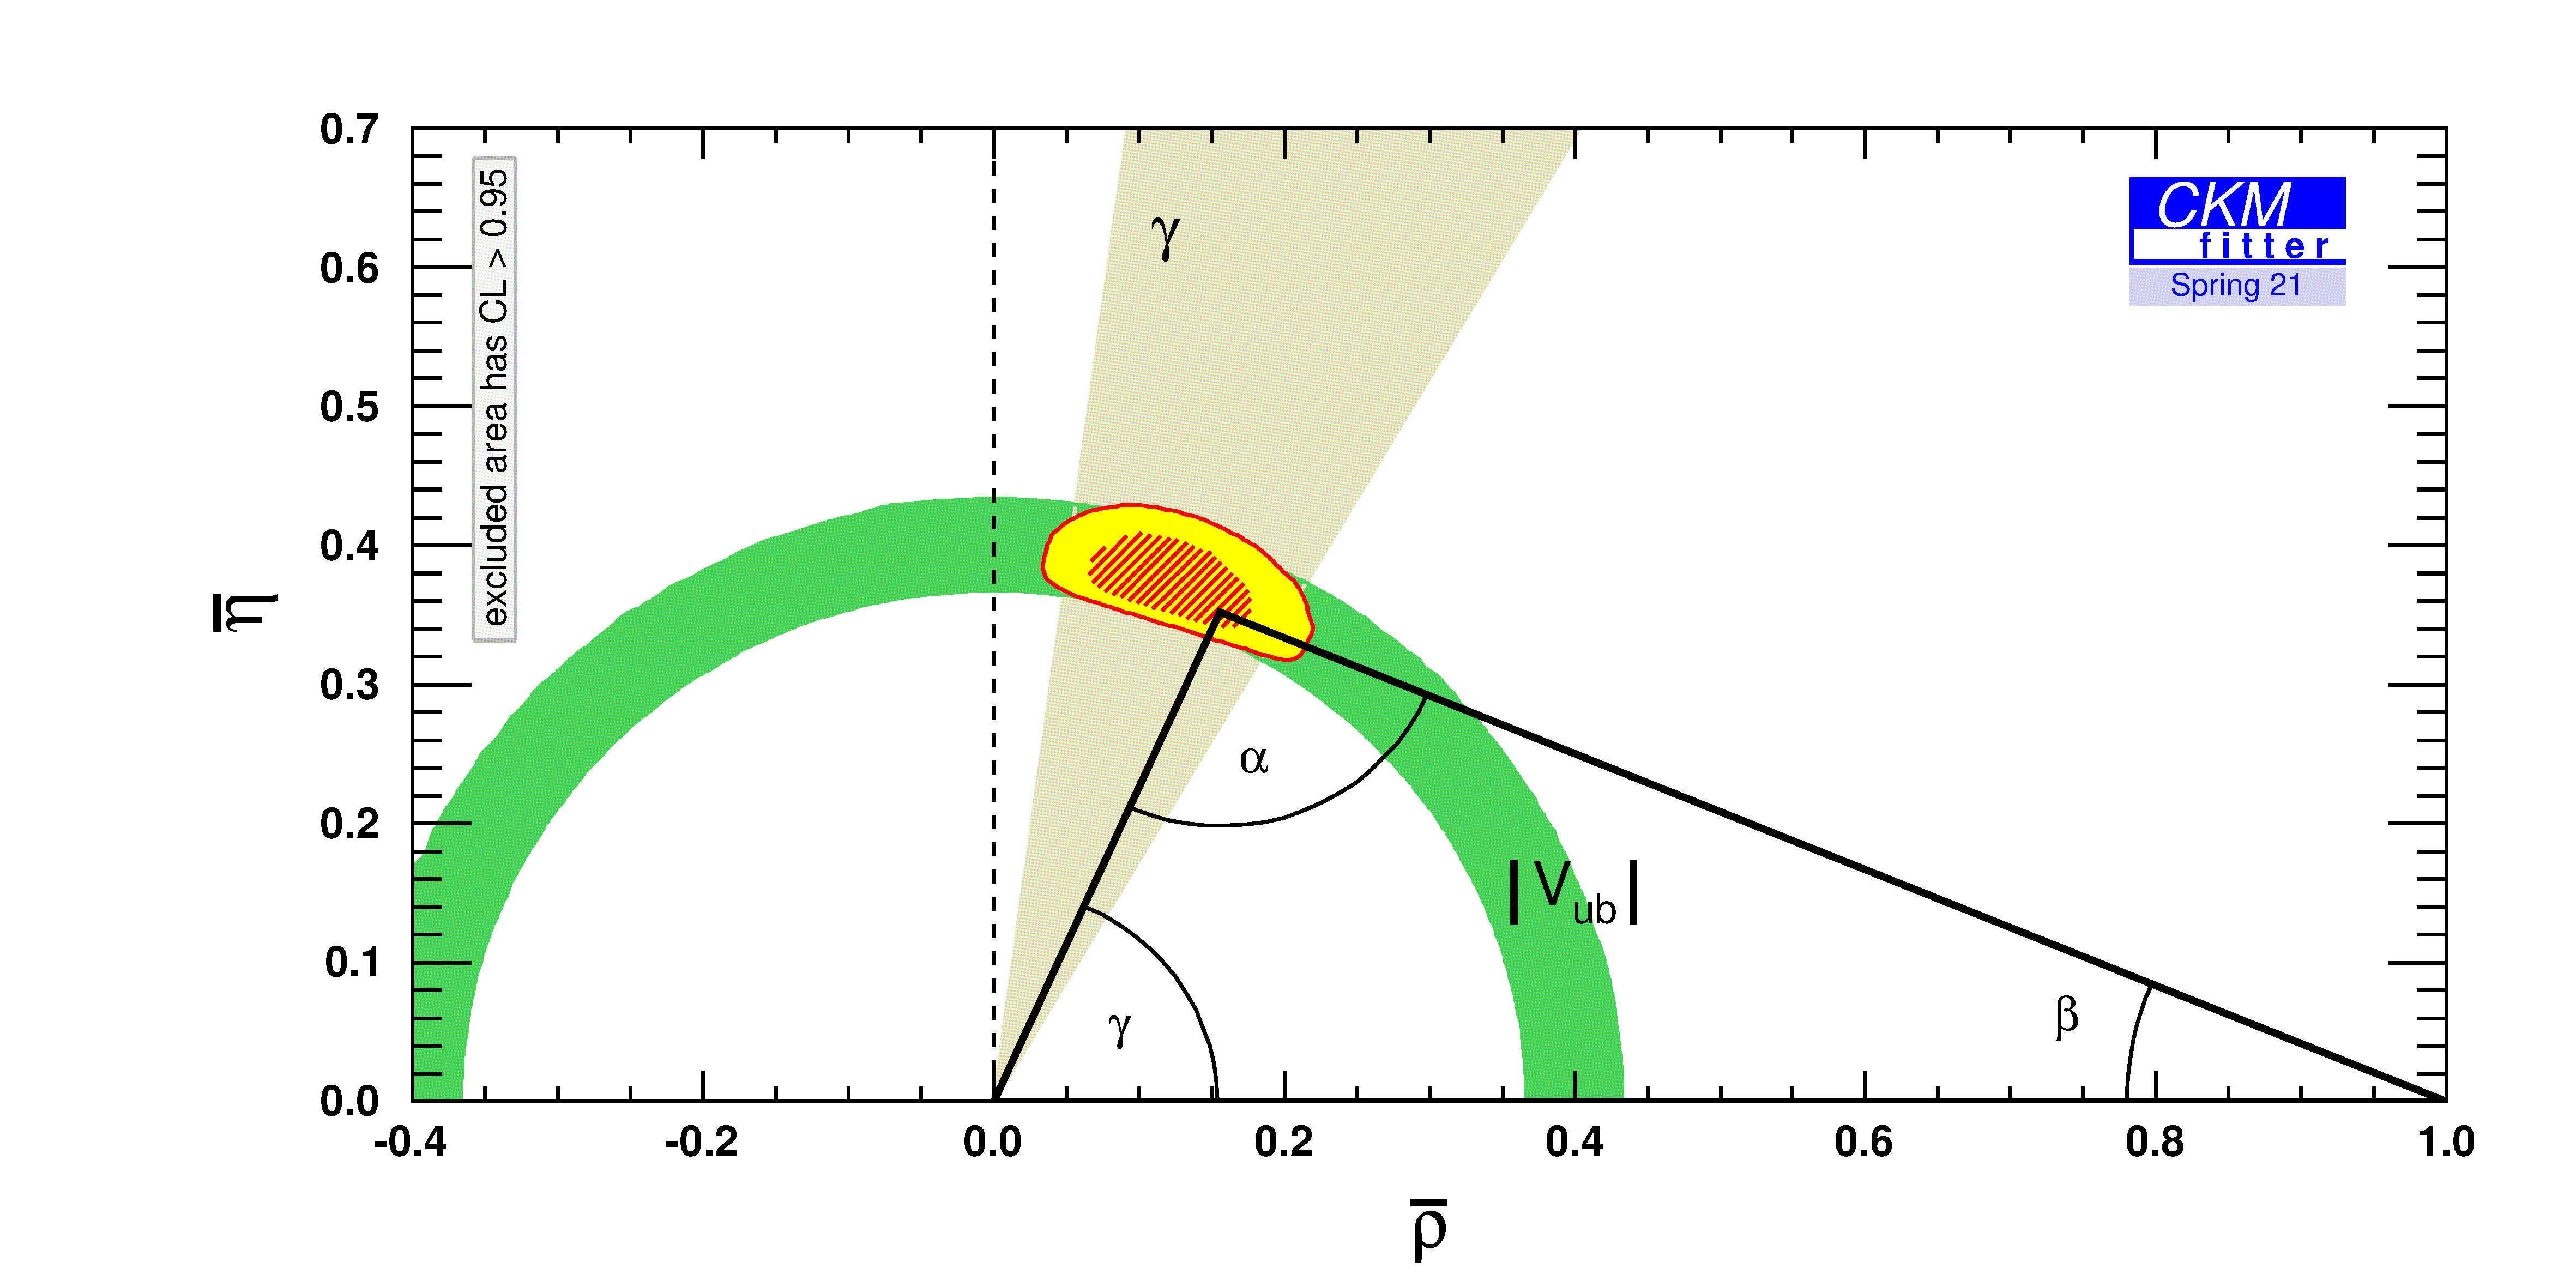
\includegraphics[width = 1.0\textwidth]{Plots/ckmfitter_tree.png}
      \caption{Tree level: $\gamma = \big(72.1^{+5.4}_{-5.7}\big)^\circ$}
    \end{subfigure}%
    \begin{subfigure}{0.5\textwidth}
      \centering
      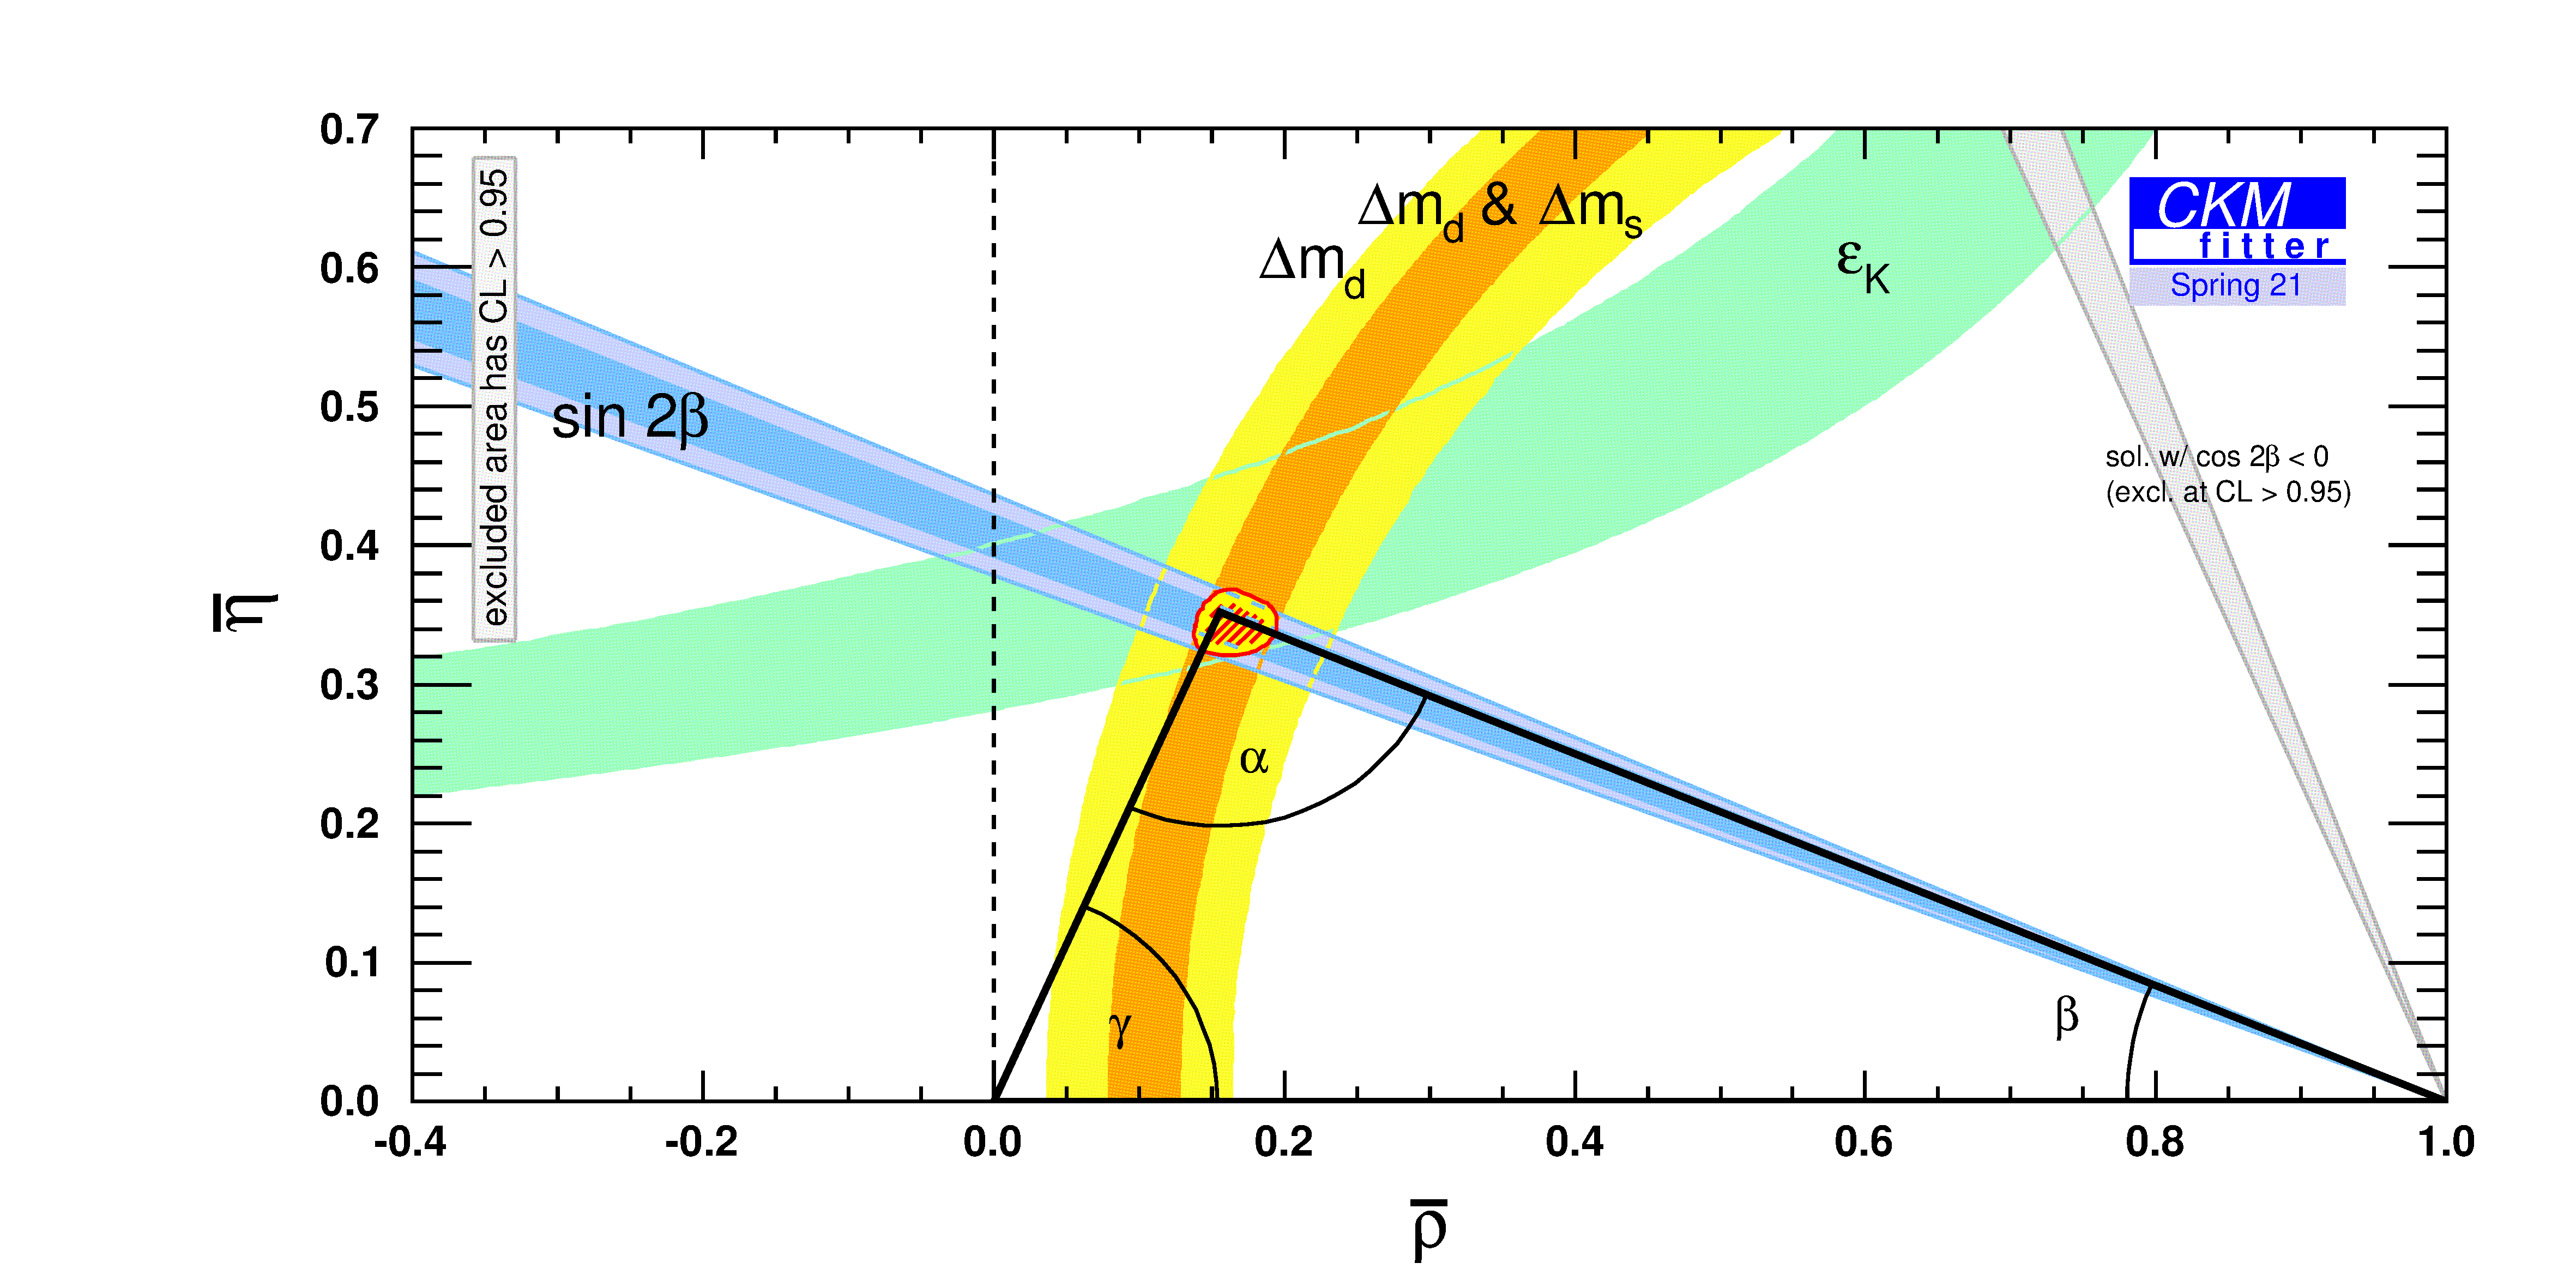
\includegraphics[width = 1.0\textwidth]{Plots/ckmfitter_loop.png}
      \caption{Loop level: $\gamma = \big(65.5^{+1.1}_{-2.7}\big)^\circ$}
    \end{subfigure}
    \vspace{-0.8cm}
    \captionsetup{justification=centering}
    \caption*{\centering\tiny CKMfitter Group (J. Charles et al.), Eur. Phys. J. C41, 1-131 (2005), updated results and plots available at: \href{http://ckmfitter.in2p3.fr}{http://ckmfitter.in2p3.fr}}
  \end{figure}
\end{frame}

\begin{frame}{Sensitivity through interference}
  \begin{center}
    \Large Measure $\gamma$ through interference effects in $B^\pm\to DK^\pm$
  \end{center}
  \begin{figure}[H]
    \centering
    \begin{subfigure}{0.5\textwidth}
      \centering
      \begin{fmffile}{fgraph/fgraph_BtoDK1}
        \setlength{\unitlength}{0.4cm}
        \begin{fmfgraph*}(6,6)
          \fmfstraight
          \fmfleft{i1,B,i2,t1,t2,t3,t9,t10}
          \fmfright{o1,D,o2,t4,t5,o3,K,o4}
          \fmflabel{$\bar{u}$}{i1}
          \fmflabel{$b$}{i2}
          \fmfv{l.d=20,l.a=180,l={$B^-$\mylbrace{30}{-8}}}{B}
          \fmflabel{$\bar{u}$}{o1}
          \fmflabel{$c$}{o2}
          \fmflabel{$\bar{u}$}{o3}
          \fmflabel{$s$}{o4}
          \fmfv{l.d=15,l.a=0,l={\myrbrace{30}{-12}}$D^0$}{D}
          \fmfv{l.d=15,l.a=0,l={\myrbrace{30}{11}}$K^-$}{K}
          \fmf{fermion}{o1,i1}
          \fmf{fermion,tension=1.5}{i2,v1}
          \fmf{fermion}{v1,o2}
          \fmf{phantom,tension=1.5}{t9,v2}
          \fmf{boson,label=$W$,label.side=left,tension=0}{v1,v2}
          \fmf{fermion}{v2,o4}
          \fmf{fermion}{o3,v2}
        \end{fmfgraph*}
      \end{fmffile}
      \vspace{0.5cm}
      \caption*{Favoured $B^-\to D^0K^-$}
    \end{subfigure}%
    \begin{subfigure}{0.5\textwidth}
      \centering
      \begin{fmffile}{fgraph/fgraph_BtoDK2}
        \setlength{\unitlength}{0.4cm}
        \begin{fmfgraph*}(6,6)
          \fmfstraight
          \fmfleft{i1,t1,t2,B,t9,t10,i2}
          \fmfright{o1,K,o2,t4,t5,o3,D,o4}
          \fmflabel{$\bar{u}$}{i1}
          \fmflabel{$b$}{i2}
          \fmfv{l.d=20,l.a=180,l={$B^-$\mylbrace{100}{-8}}}{B}
          \fmflabel{$\bar{u}$}{o1}
          \fmflabel{$s$}{o2}
          \fmflabel{$\bar{c}$}{o3}
          \fmflabel{$u$}{o4}
          \fmfv{l.d=15,l.a=0,l={\myrbrace{30}{13}}$\bar{D^0}$}{D}
          \fmfv{l.d=15,l.a=0,l={\myrbrace{30}{-13}}$K^-$}{K}
          \fmf{fermion}{o1,i1}
          \fmf{fermion,tension=1.5}{i2,v1}
          \fmf{fermion}{v1,o4}
          \fmf{phantom,tension=1.5}{t2,v2}
          \fmf{boson,label=$W$,label.side=left,tension=0}{v1,v2}
          \fmf{fermion}{v2,o2}
          \fmf{fermion}{o3,v2}
        \end{fmfgraph*}
      \end{fmffile}
      \vspace{0.5cm}
      \caption*{Suppressed $B^-\to\bar{D^0}K^-$}
    \end{subfigure}
  \end{figure}
  \vspace{-0.3cm}
  \begin{itemize}
    \item{Superposition of $D^0$ and $\bar{D^0}$}
    \begin{itemize}
      \item{Consider $D^0$/$\bar{D^0}$ decays to the same final state, such as $D\to K^+K^-$}
    \end{itemize}
    \item{$b\to u\bar{c}s$ and $b\to c\bar{u}s$ interference $\to$ Sensitivity to $\gamma$}
  \end{itemize}
  \vspace{-0.3cm}
  \begin{center}
    $\mathcal{A}(B^-)=\mathcal{A}_B\Big(\mathcal{A}_{D^0} + r_Be^{i(\delta_B - \gamma)}\mathcal{A}_{\bar{D^0}}\Big)$ \\
    $\mathcal{A}(B^+)=\mathcal{A}_B\Big(\mathcal{A}_{\bar{D^0}} + r_Be^{i(\delta_B + \gamma)}\mathcal{A}_{D^0}\Big)$ \\
  \end{center}
\end{frame}

\begin{frame}{Multi-body charm decays}
  \vspace{0.0cm}
  {\large In this presentation, four-body charm decays are considered:}
  \begin{center}
    {\Large
    $D^0\to K^+K^-\pi^+\pi^-$ \\~\\
    $D^0\to\pi^+\pi^-\pi^+\pi^-$}
  \end{center}
  \vspace{0.2cm}
  Note: Such decays have a five-dimensional phase space!
  \scriptsize
  \begin{center}
    \begin{minipage}{0.6\textwidth}
      \begin{block}{\centering Degrees of freedom for an $N$-body decay}
        \vspace{-0.5cm}
        \begin{align*}
          &4N \text{ (momentum components)} \\
          -\;&N \text{ ($E_i^2-p_i^2=m_i^2$)} \\
          -\;&4 \text{ (energy-momentum conservation)} \\
          -\;&3 \text{ (choice of frame)} \\[-0.1cm]
          \cline{1-2}\\[-0.5cm]
          =\;&3N-7 \text{ degrees of freedom}
        \end{align*}
      \end{block}
    \end{minipage}
  \end{center}
\end{frame}

\begin{frame}{Previous studies of $\gamma$ with $B^\pm\to DK^\pm$, $D\to K^+K^-\pi^+\pi^-$}
  \vspace{0.0cm}
  \begin{enumerate}
    \setlength\itemsep{1.2em}
    \item{First proposed by J. Rademacker and G. Wilkinson:}
    \begin{itemize}
      \item{\href{https://arxiv.org/abs/hep-ph/0611272}{Physics Letters B \textbf{647} (2007) 400}}
      \item{Amplitude model by FOCUS}
      \item{Expected $\gamma$ precision from amplitude fit with $1000$ candidates: $14^\circ$}
    \end{itemize}
    \item{CLEO amplitude analysis:}
    \begin{itemize}
      \item{\href{https://arxiv.org/abs/1201.5716}{Phys. Rev. D \textbf{85} (2012) 122002}}
      \item{Expected $\gamma$ precision from amplitude fit with $2000$ candidates: $11^\circ$}
    \end{itemize}
    \item{State of the art amplitude analysis by LHCb:}
    \begin{itemize}
      \item{\href{https://arxiv.org/abs/1811.08304}{JHEP \textbf{02} (2019) 126}}
    \end{itemize}
    \item{Model-dependent measurement by LHCb:}
    \begin{itemize}
      \item{\href{https://arxiv.org/abs/2301.10328}{Eur. Phys. J. C \textbf{83} 547 (2023)}}
      \item{Optimised binning scheme using LHCb amplitude model}
    \end{itemize}
  \end{enumerate}
\end{frame}

\begin{frame}{Inputs to $D^0\to K^+K^-\pi^+\pi^-$ mode}
  \vspace{0.0cm}
  \begin{center}
    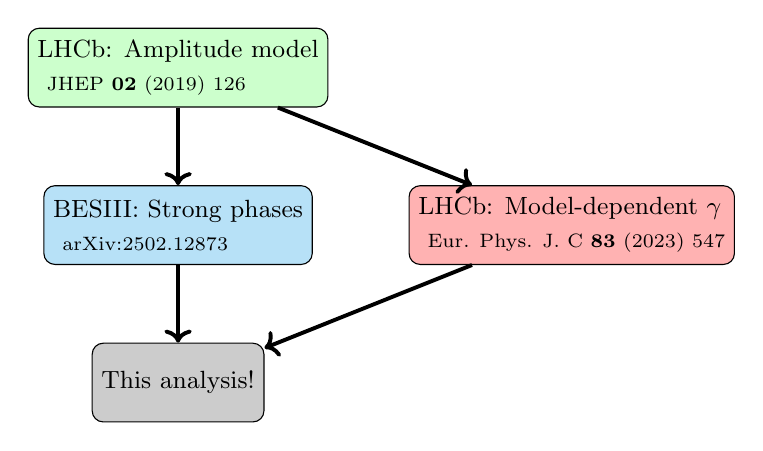
\begin{tikzpicture}[node distance=2cm]
      \node(n1)[rectangle,fill=green!20,rounded corners,draw=black,midway,minimum height=1cm,minimum width=2cm,align=left]{\small LHCb: Amplitude model\\~\scriptsize JHEP \textbf{02} (2019) 126};
      \node(n3)[rectangle,fill=Cerulean!30,rounded corners,draw=black,minimum height=1cm,below of=n1,minimum width=2cm,align=left]{\small BESIII: Strong phases\\~\scriptsize arXiv:2502.12873};
      \node(n2)[rectangle,fill=red!30,rounded corners,draw=black,minimum height=1cm,right of=n3,minimum width=2cm,align=left,xshift=3cm]{\small LHCb: Model-dependent $\gamma$\\~\scriptsize Eur. Phys. J. C \textbf{83} (2023) 547};
      \node(n4)[rectangle,fill=black!20,rounded corners,draw=black,minimum height=1cm,below of=n3,minimum width=2cm,align=left]{\small This analysis!};
      \draw[->,line width=0.5mm](n1)--(n2);
      \draw[->,line width=0.5mm](n1)--(n3);
      \draw[->,line width=0.5mm](n2)--(n4);
      \draw[->,line width=0.5mm](n3)--(n4);
    \end{tikzpicture}
  \end{center}
  \vspace{0.0cm}
\end{frame}

\begin{frame}{Previous studies of $\gamma$ with $B^\pm\to DK^\pm$, $D\to\pi^+\pi^-\pi^+\pi^-$}
  \vspace{0.0cm}
  \begin{enumerate}
    \setlength\itemsep{1.2em}
    \item{CLEO amplitude analysis:}
    \begin{itemize}
      \item{\href{https://arxiv.org/abs/1703.08505}{JHEP \textbf{05} (2017) 143}}
    \end{itemize}
    \item{CLEO-c strong-phase measurement:}
    \begin{itemize}
      \item{\href{https://arxiv.org/abs/1709.03467}{JHEP \textbf{01} (2018) 144}}
      \item{Expected $\gamma$ statistical (systematic) precision with $2\times 5$ bins is $9.7^\circ$ ($7.4^\circ$)}
    \end{itemize}
    \item{For this LHCb publication:}
    \begin{itemize}
      \item{New amplitude model from BESIII \href{https://iopscience.iop.org/article/10.1088/1674-1137/ad3d4d}{Chin. Phys. C \textbf{48} (2024) 083001}}
      \item{$\to$ Motivation to perform $c_i$/$s_i$ measurements using a new binning scheme \href{https://journals.aps.org/prd/abstract/10.1103/PhysRevD.110.112008}{Phys. Rev. D \textbf{110} (2024) 112008}}
      \item{Results presented from both CLEO-c and BESIII binning schemes}
      \item{Selection unified between Bristol and Oxford}
    \end{itemize}
  \end{enumerate}
\end{frame}

\begin{frame}{Inputs to $D^0\to\pi^+\pi^-\pi^+\pi^-$ mode}
  \vspace{0.0cm}
  \begin{center}
    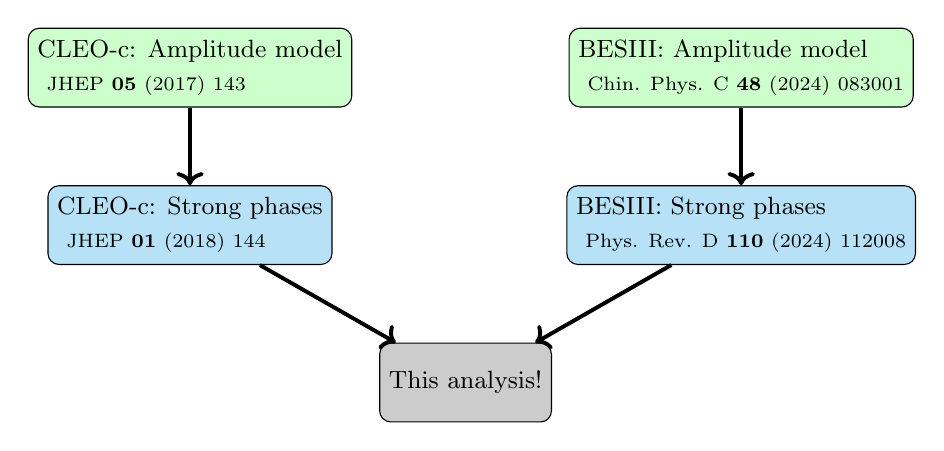
\begin{tikzpicture}[node distance=2cm]
      \node(n1)[rectangle,fill=green!20,rounded corners,draw=black,midway,minimum height=1cm,minimum width=2cm,align=left]{\small CLEO-c: Amplitude model\\~\scriptsize JHEP \textbf{05} (2017) 143};
      \node(n2)[rectangle,fill=green!20,rounded corners,draw=black,midway,minimum height=1cm,minimum width=2cm,align=left,right of=n1,xshift=5cm]{\small BESIII: Amplitude model\\~\scriptsize Chin. Phys. C \textbf{48} (2024) 083001};
      \node(n3)[rectangle,fill=Cerulean!30,rounded corners,draw=black,minimum height=1cm,below of=n1,minimum width=2cm,align=left]{\small CLEO-c: Strong phases\\~\scriptsize JHEP \textbf{01} (2018) 144};
      \node(n4)[rectangle,fill=Cerulean!30,rounded corners,draw=black,minimum height=1cm,below of=n2,minimum width=2cm,align=left]{\small BESIII: Strong phases\\~\scriptsize Phys. Rev. D \textbf{110} (2024) 112008};
      \node(n5)[rectangle,fill=black!20,rounded corners,draw=black,minimum height=1cm,below of=n4,minimum width=2cm,xshift=-3.5cm,align=left]{\small This analysis!};
      \draw[->,line width=0.5mm](n1)--(n3);
      \draw[->,line width=0.5mm](n2)--(n4);
      \draw[->,line width=0.5mm](n3)--(n5);
      \draw[->,line width=0.5mm](n4)--(n5);
    \end{tikzpicture}
  \end{center}
  \vspace{0.0cm}
\end{frame}

\begin{frame}{Selection of $B^\pm\to DK^\pm$, $D\to\pi^+\pi^-\pi^+\pi^-$}
  \vspace{0.0cm}
  {Selection of $B^\pm\to[\pi^+\pi^-\pi^+\pi^-]_D h^\pm$ is mostly similar to that in phase-space integrated measurement \href{https://link.springer.com/article/10.1140/epjc/s10052-023-11560-5}{Eur. Phys. J. C \textbf{83} 547 (2023)}}
  \vspace{0.5cm}
  \begin{itemize}
    \setlength\itemsep{2.0em}
    \item{Minor differences adapted for binned measurement:}
    \item{Flight significance cut loosened from $4$ to $2$}
    \begin{itemize}
      \item{Phase-space binned analysis is less sensitive to charmless background}
    \end{itemize}
    \item{Hadrons from $D^0$: \texttt{ProbNNpi*(1-ProbNNk) > 0.05}}
    \begin{itemize}
      \item{Highly efficient at rejecting combinatorial background}
      \item{Phase-space binned analysis benefits from higher purity in low-yield bins}
    \end{itemize}
  \end{itemize}
\end{frame}

\begin{frame}{Phase-space integrated CP observables}
  \begin{center}
    {\large Phase-space integrated study of $\gamma$: \\
    Charged asymmetries measured for $D\to K^+K^-\pi^+\pi^-$ and $D\to\pi^+\pi^-\pi^+\pi^-$ in Eur. Phys. J. C \textbf{83} 547 (2023)}
  \end{center}
  \vspace{-0.4cm}
  \begin{figure}
    \centering
    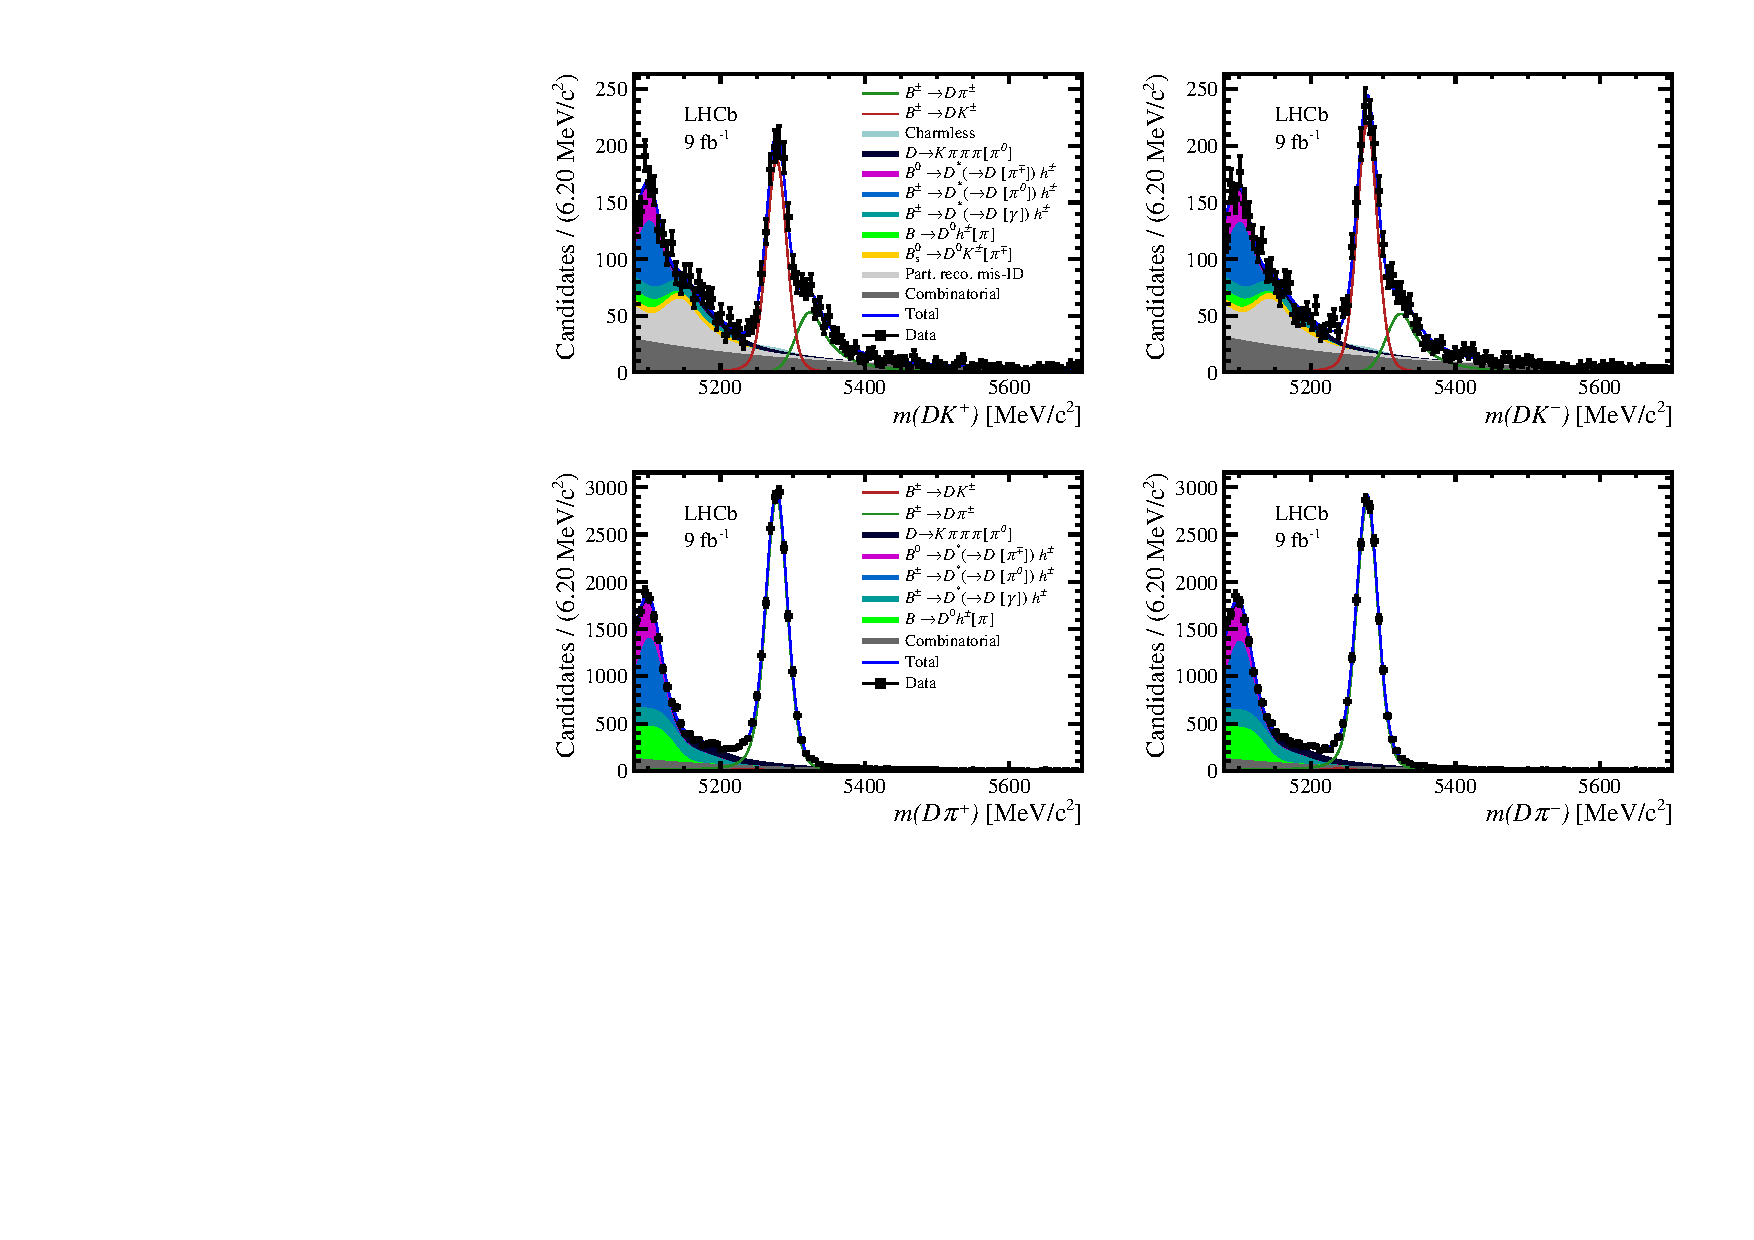
\includegraphics[width = 0.9\textwidth,trim={0 7cm 0 0},clip=true]{Plots/d2kkpipi_fiveL_allDP_GLW.pdf}
    \caption*{$D\to K^+K^-\pi^+\pi^-$}
  \end{figure}
  \vspace{-0.5cm}
  \begin{itemize}
    \item{$B^\pm\to[h^+h^-\pi^+\pi^-]_Dh^\pm$ asymmetries:}
    \begin{itemize}
      \item[-]{$D\to K^+K^-\pi^+\pi^-$: $\mathcal{A} = 0.095 \pm 0.023 \pm 0.002$}
      \item[-]{$D\to\pi^+\pi^-\pi^+\pi^-$: $\mathcal{A} = 0.061 \pm 0.013 \pm 0.002$}
    \end{itemize}
  \end{itemize}
\end{frame}

\begin{frame}{Phase-space integrated CP observables}
  \begin{center}
    {\large Phase-space integrated study of $\gamma$: \\
    Charged asymmetries measured for $D\to K^+K^-\pi^+\pi^-$ and $D\to\pi^+\pi^-\pi^+\pi^-$ in Eur. Phys. J. C \textbf{83} 547 (2023)}
  \end{center}
  \vspace{-0.4cm}
  \begin{figure}
    \centering
    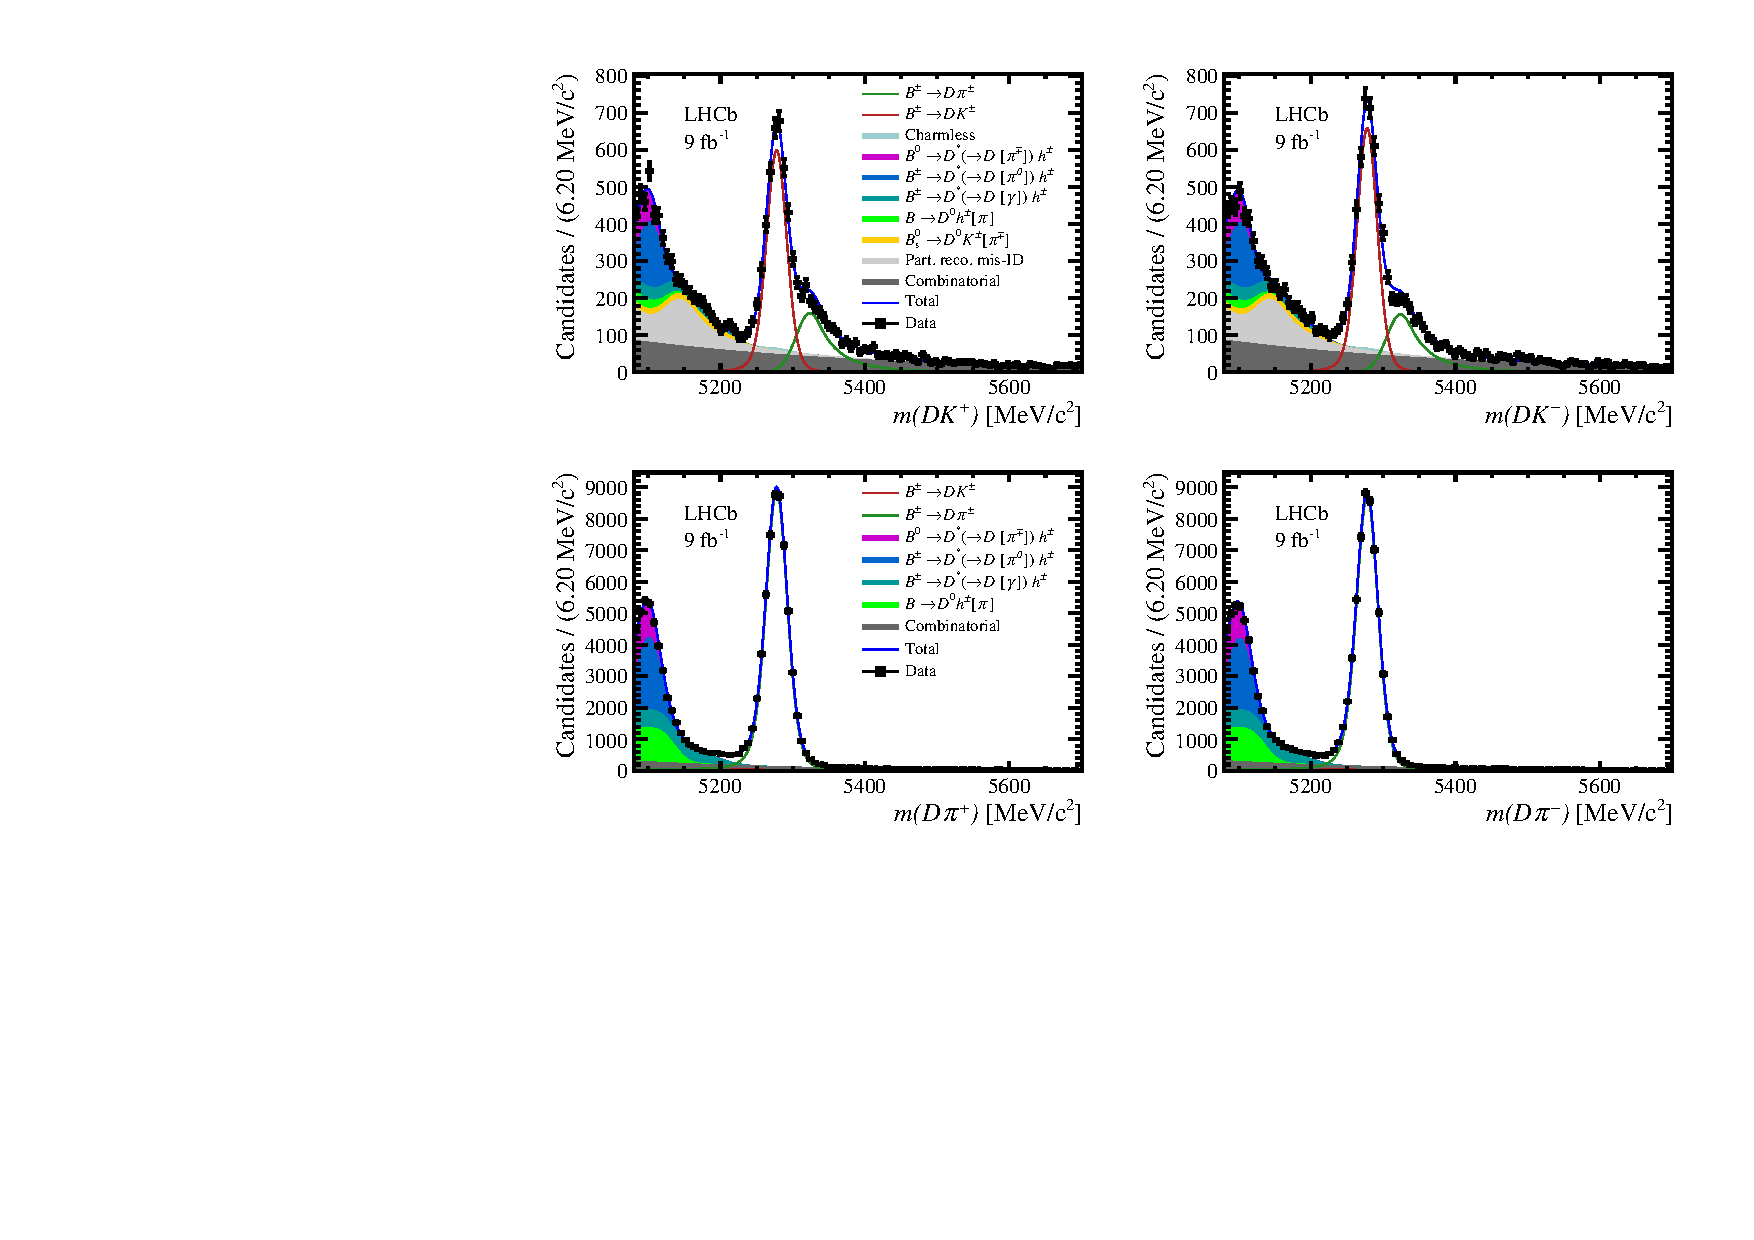
\includegraphics[width = 0.9\textwidth,trim={0 7cm 0 0},clip=true]{Plots/d2pipipipi_fiveL_allDP_GLW.pdf}
    \caption*{$D\to\pi^+\pi^-\pi^+\pi^-$}
  \end{figure}
  \vspace{-0.5cm}
  \begin{itemize}
    \item{$B^\pm\to[h^+h^-\pi^+\pi^-]_Dh^\pm$ asymmetries:}
    \begin{itemize}
      \item[-]{$D\to K^+K^-\pi^+\pi^-$: $\mathcal{A} = 0.095 \pm 0.023 \pm 0.002$}
      \item[-]{$D\to\pi^+\pi^-\pi^+\pi^-$: $\mathcal{A} = 0.061 \pm 0.013 \pm 0.002$}
    \end{itemize}
  \end{itemize}
\end{frame}

\begin{frame}[fragile]{Multi-body $D$ decays}
  \begin{center}
    Main focus of this talk: Discuss phase-space binned analysis of $D\to h^+h^-\pi^+\pi^-$
  \end{center}
  \vspace{-0.3cm}
  \begin{itemize}
    \setlength\itemsep{0.5em}
    \item{Strong-phase difference $\delta_D$ is a function of phase space}
    \item{Compare yields of $B^+$ and $B^-$ and determine the asymmetry \underline{in local phase space regions}, known as phase-space bins}
  \end{itemize}
  \begin{equation*}
    \begin{tikzcd}[column sep=huge]
      & D^0K^- \arrow[dr, bend left = 25, "\mathcal{A}_{D^0}(\Phi)"] & \\
      B^- \arrow[ur, bend left, "\mathcal{A}_B"] \arrow[dr, bend right, "\mathcal{A}_B r_B e^{i(\delta_B - \gamma)}"'] & [5cm] & DK^- \\
      & \bar{D^0}K^- \arrow[ur, bend right = 25, "\mathcal{A}_{\bar{D^0}}(\Phi)"'] & \\
    \end{tikzcd}
  \end{equation*}
  \vspace{-0.9cm}
  \begin{align*}
    \lvert\mathcal{A}(B^-)\lvert^2&\propto\lvert\mathcal{A}_{D^0}(\Phi)\lvert^2 + r_B^2\lvert\mathcal{A}_{\bar{D^0}}(\Phi)\lvert^2 \\
    &+ 2r_B\lvert\mathcal{A}_{D^0}(\Phi)\lvert\lvert\mathcal{A}_{\bar{D^0}}(\Phi)\lvert\cos(\delta_B - \gamma + \delta_D)
  \end{align*}
\end{frame}

\begin{frame}{The BPGGSZ method}
\begin{center}
    \begin{minipage}{0.6\textwidth}
      \begin{block}{Event yield in bin $i$}
        \footnotesize
        $N^-_i = h_{B^-}\big(F_i + (x_-^2 + y_-^2)\bar{F_i} + 2\sqrt{F_i\bar{F_i}}(x_-c_i + y_-s_i)\big)$ \\
        $N^+_{-i} = h_{B^+}\big(F_i + (x_+^2 + y_+^2)\bar{F_i} + 2\sqrt{F_i\bar{F_i}}(x_+c_i + y_+s_i)\big)$
      \end{block}
    \end{minipage}
  \end{center}
  \begin{itemize}
    \item{CP observables:}
    \begin{itemize}
      \item{$x_\pm^{DK} = r_B^{DK}\cos(\delta_B^{DK}\pm\gamma)$, \quad $y_\pm^{DK} = r_B^{DK}\sin(\delta_B^{DK}\pm\gamma)$}
      \item{$x_\xi^{D\pi} = \Re(\xi^{D\pi})$, $y_\xi^{D\pi} = \Im(\xi^{D\pi})$ $\quad\quad\Big(\xi^{D\pi} = \frac{r_B^{D\pi}}{r_B^{DK}}e^{i(\delta_B^{D\pi} - \delta_B^{DK})}\Big)$}
    \end{itemize}
    \item{Fractional bin yield:}
    \begin{itemize}
      \item{$F_i = \frac{\int_i\dd{\Phi}|\mathcal{A}(D^0)|^2}{\sum_j\int_j\dd{\Phi}\abs{\mathcal{A}(D^0)}^2}$}
      \item{Floated in the fit, mostly constrained by $B^\pm\to D\pi^\pm$}
    \end{itemize}
  \end{itemize}
  \begin{itemize}
    \item{Amplitude-averaged strong phases:}
    \begin{center}
      $c_i = \frac{\int_i\dd{\Phi}|\mathcal{A}(D^0)||\mathcal{A}(\bar{D^0})|\cos(\delta_D)}{\sqrt{\int_i\dd{\Phi}\abs{\mathcal{A}(D^0)}^2\int_i\dd{\Phi}\abs{\mathcal{A}(\bar{D^0})}^2}}$ \quad $s_i = \frac{\int_i\dd{\Phi}|\mathcal{A}(D^0)||\mathcal{A}(\bar{D^0})|\sin(\delta_D)}{\sqrt{\int_i\dd{\Phi}\abs{\mathcal{A}(D^0)}^2\int_i\dd{\Phi}\abs{\mathcal{A}(\bar{D^0})}^2}}$
    \end{center}
  \end{itemize}
\end{frame}

\begin{frame}{$D^0\to K^+K^-\pi^+\pi^-$ binning scheme}
  \begin{itemize}
    \setlength\itemsep{0.5em}
    \item{Interpretation of $\gamma$ from the multi-body charm decays require external inputs of the charm strong-phase differences}
    \item{Measure model-independent strong-phases at a charm factory, such as BESIII, using an optimised binning scheme}
  \end{itemize}
  \begin{figure}
    \centering
    \begin{subfigure}{0.5\textwidth}
      \centering
      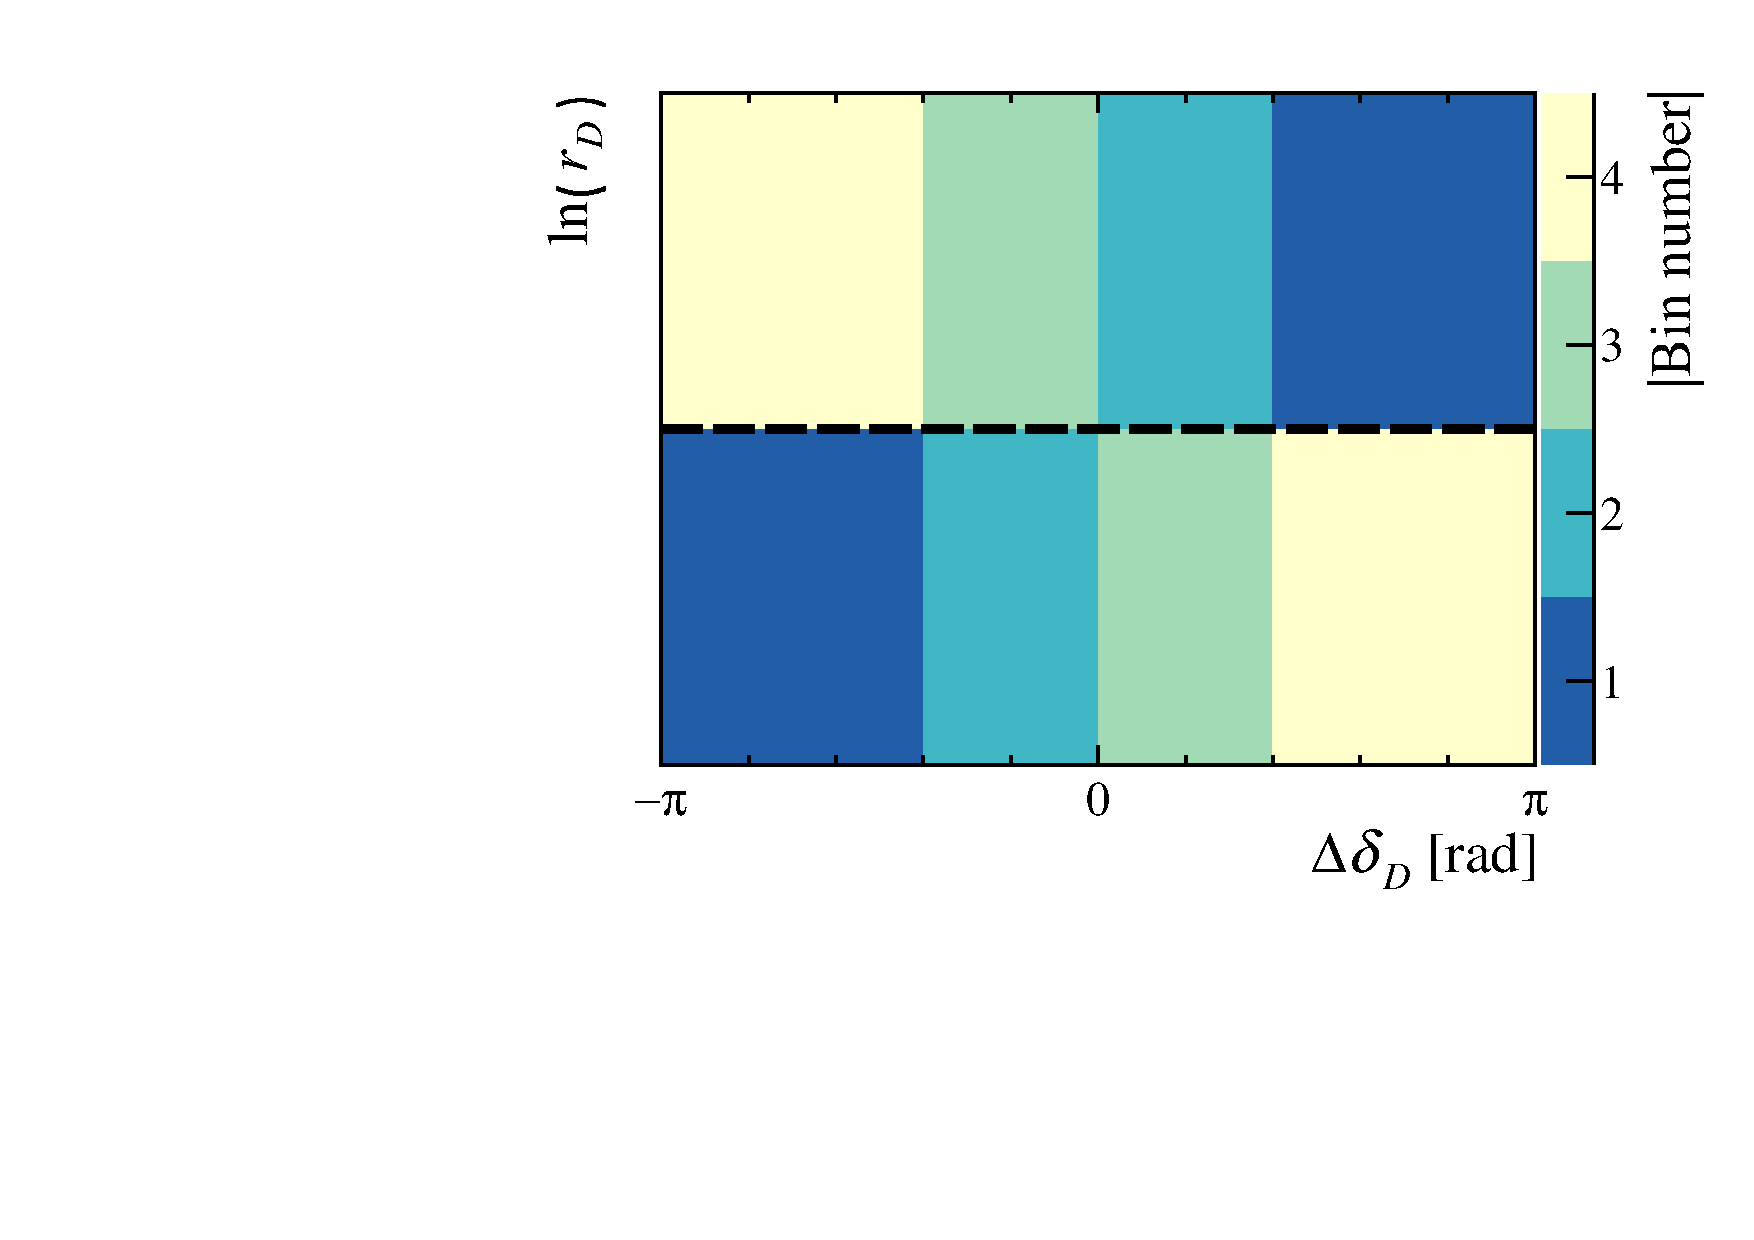
\includegraphics[height = 3.5cm]{Plots/BinningSchemePlot_4Bins.pdf}
      \vspace{-0.3cm}
      \caption*{4 bins}
    \end{subfigure}%
    \begin{subfigure}{0.5\textwidth}
      \centering
      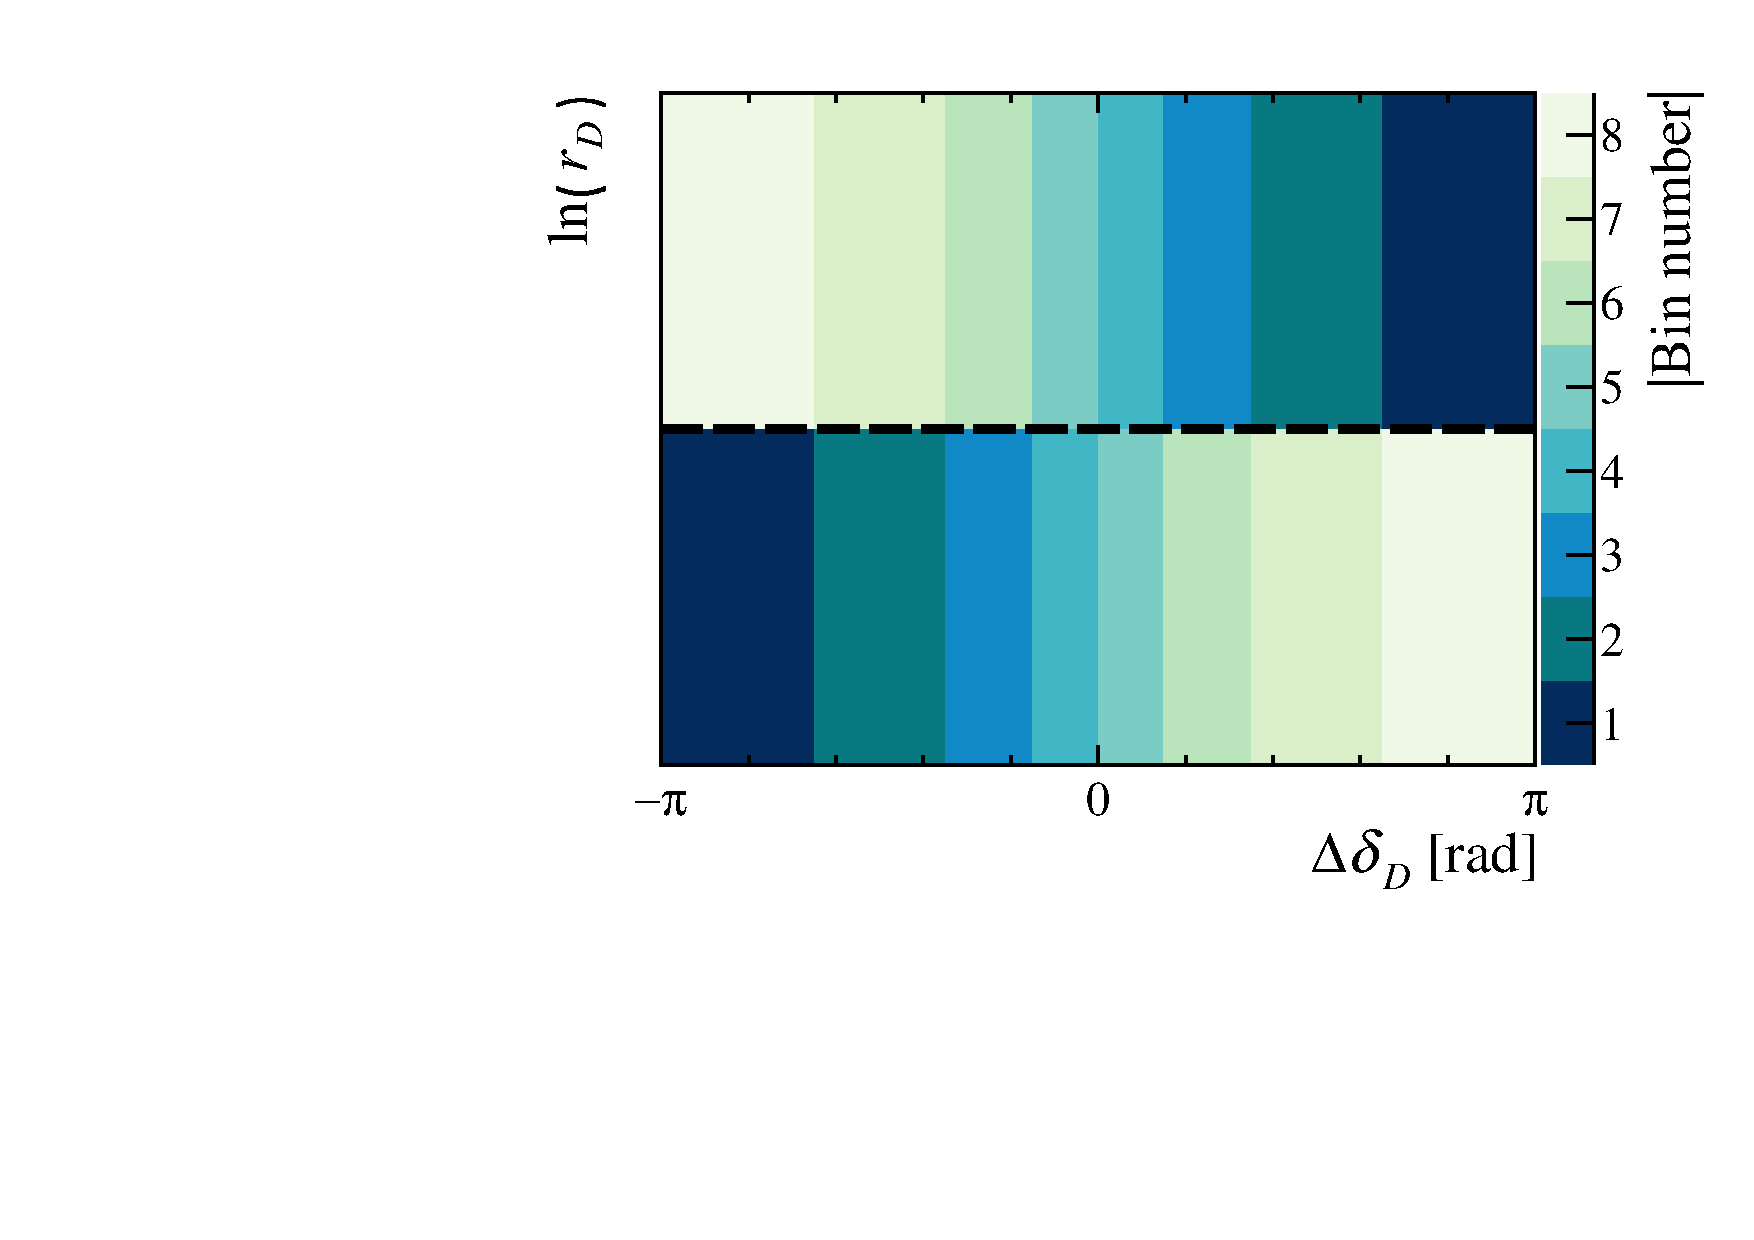
\includegraphics[height = 3.5cm]{Plots/BinningSchemePlot_8Bins.pdf}
      \vspace{-0.3cm}
      \caption*{8 bins}
    \end{subfigure}
    \caption*{$D^0\to K^+K^-\pi^+\pi^-$ binning scheme}
  \end{figure}
\end{frame}

\begin{frame}{Model-dependent measurement with $D\to K^+K^-\pi^+\pi^-$}
  \begin{center}
    \large From the phase-space binned asymmetries, we obtain:\\
    \vspace{0.2cm}
    $\gamma = (116^{+12}_{-14})^\circ$
  \end{center}
  \vspace{-0.2cm}
  \begin{figure}[htb]
    \centering
    \begin{subfigure}{0.5\textwidth}
      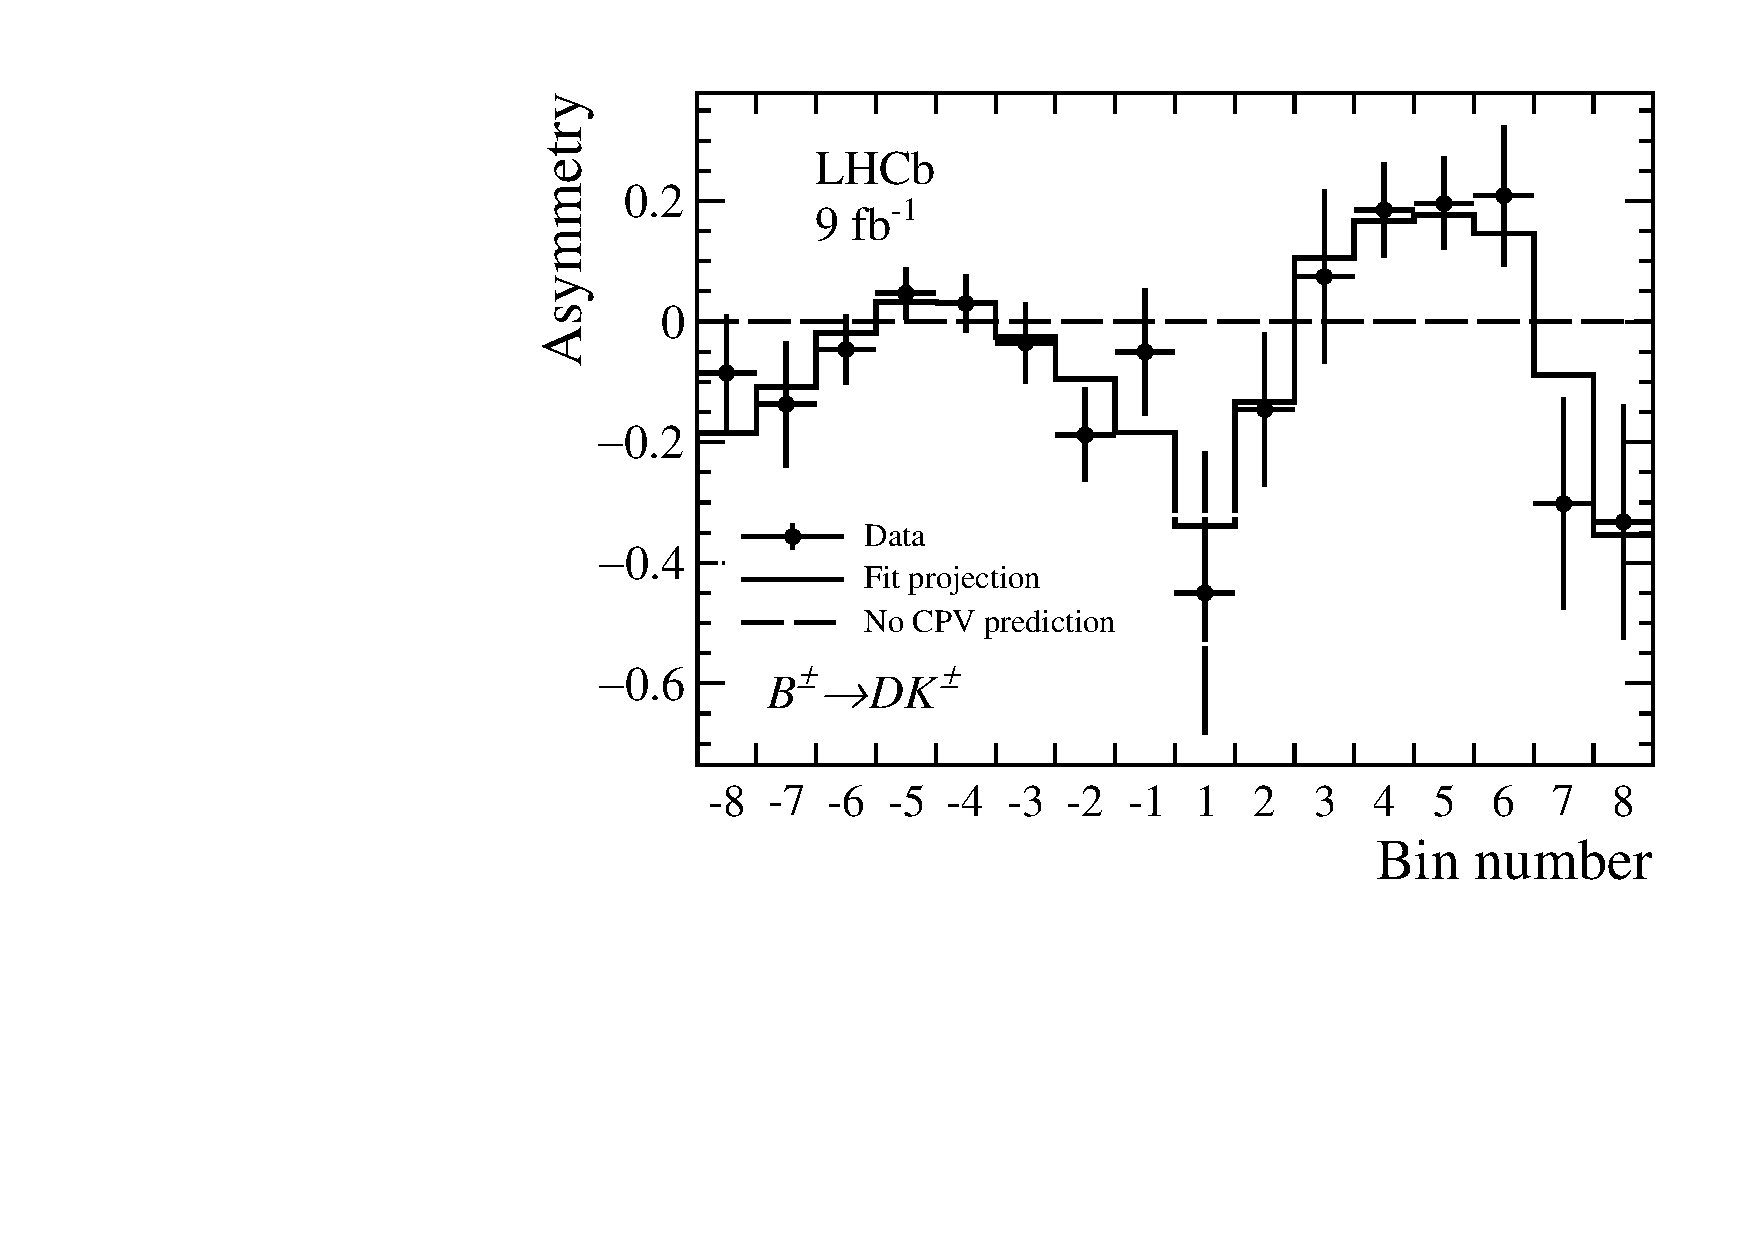
\includegraphics[width=1\textwidth]{Plots/BinAsymmetries_dk_ModelDependent.pdf}
    \end{subfigure}%
    \begin{subfigure}{0.5\textwidth}
      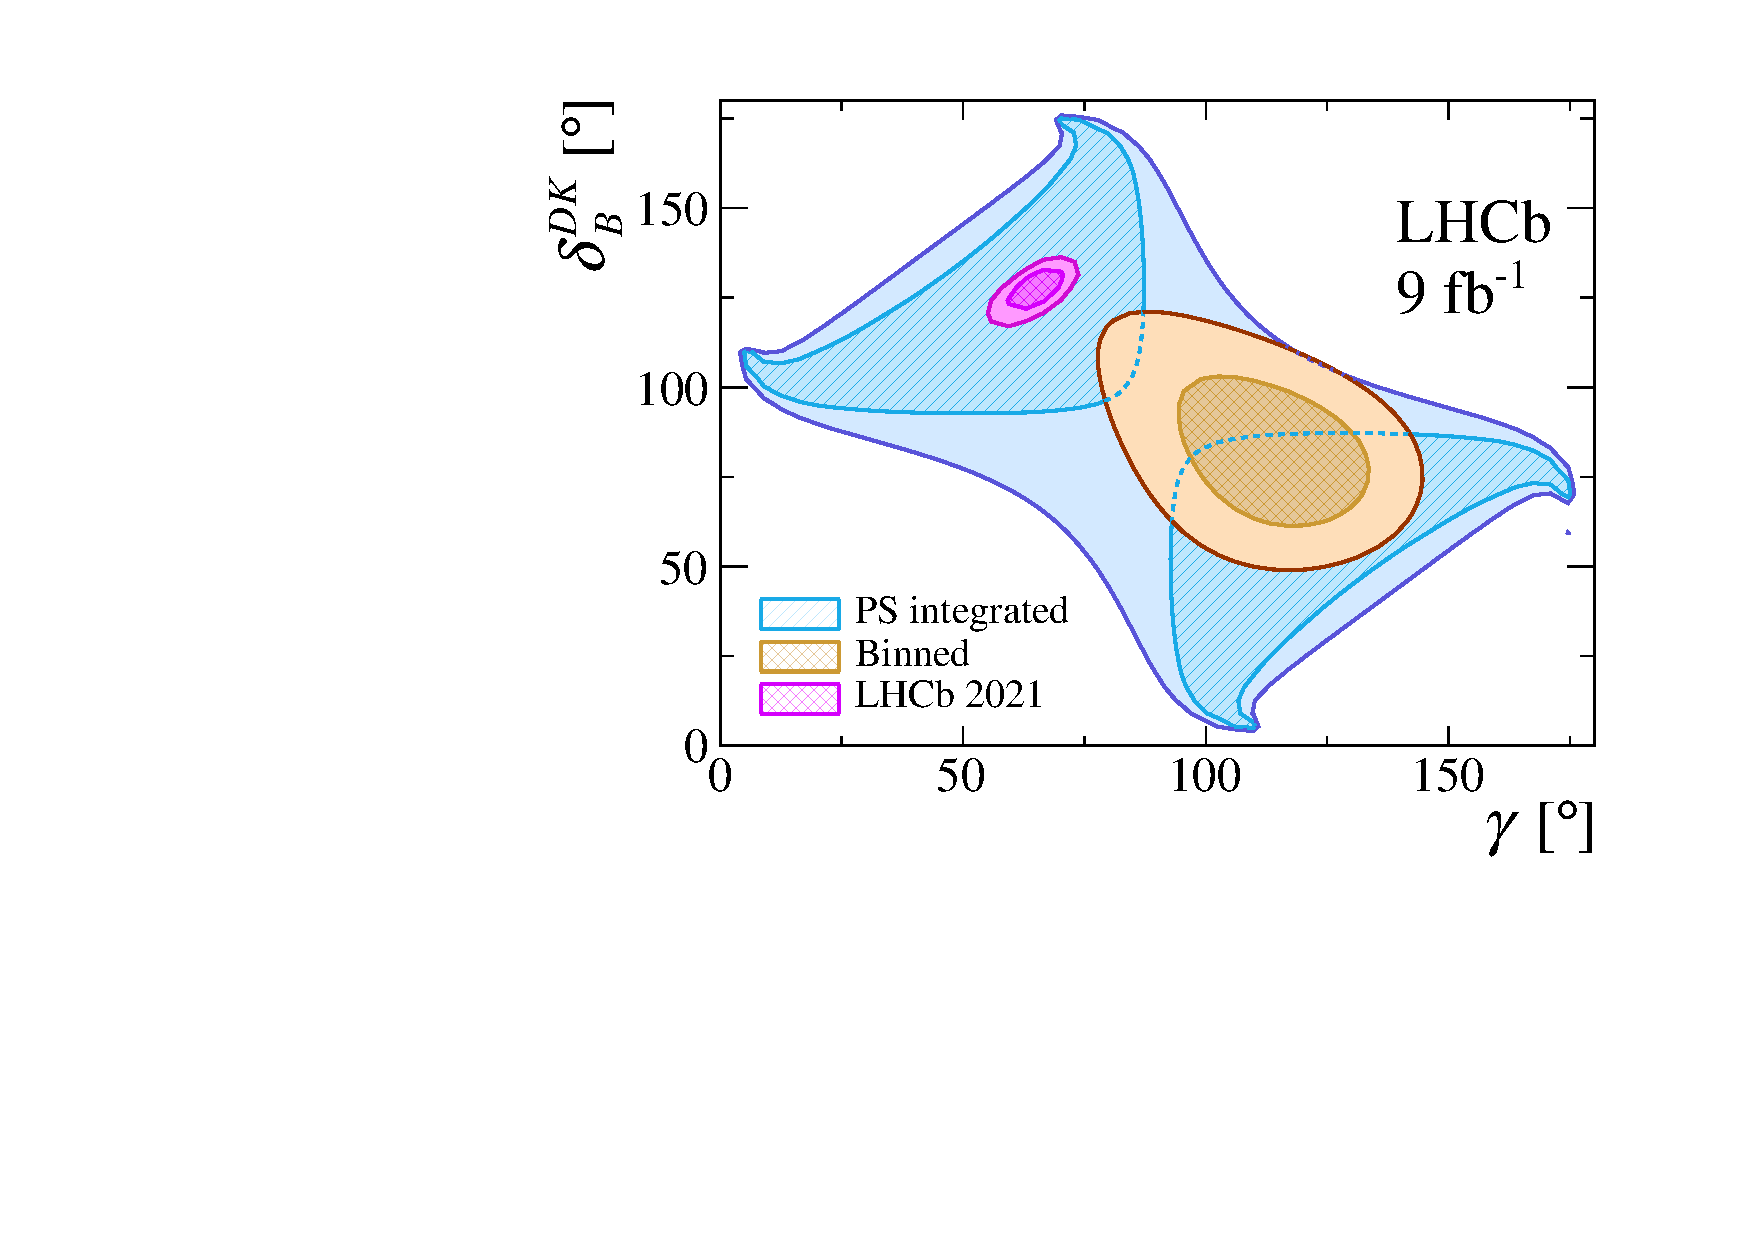
\includegraphics[width=1\textwidth]{Plots/gammacharm_lhcb_KKpipi_GLW_KKpipi_GGSZ_lhcb_2020_beauty_and_charm_g_d_dk_ModelDependent.pdf}
    \end{subfigure}
    \vspace{-0.5cm}
    \caption*{\tiny\href{https://link.springer.com/article/10.1140/epjc/s10052-023-11560-5}{Eur. Phys. J. C \textbf{83}, 547 (2023)}}
  \end{figure}
  \vspace{-0.5cm}
  \begin{center}
    {\large How will this evolve with model-independent BESIII inputs? Will the $3\sigma$ tension reduce?}
  \end{center}
\end{frame}

\begin{frame}{Motivation for this analysis}
  \begin{center}
    {\Large What is new from previous analysis of $K^+K^-\pi^+\pi^-$?}
  \end{center}
  \begin{itemize}
    \setlength\itemsep{1.0em}
    \item{New binned strong-phase analyses of $D\to K^+K^-\pi^+\pi^-$ and $D\to\pi^+\pi^-\pi^+\pi^-$ have recently been made public by BESIII}
    \begin{itemize}
      \item{$D^0\to KK\pi\pi$: \href{https://arxiv.org/abs/2502.12873}{arXiv:2502.12873}}
      \item{$D^0\to \pi\pi\pi\pi$: \href{https://journals.aps.org/prd/abstract/10.1103/PhysRevD.110.112008}{Phys. Rev. D \textbf{110} (2024) 112008}}
      \item{For $D\to\pi^+\pi^-\pi^+\pi^-$, these improve in precision on earlier binned study made with CLEO-c data \href{https://link.springer.com/article/10.1007/JHEP01(2018)144}{JHEP \textbf{01} (2018) 144}}
    \end{itemize}
    \item{Make first binned model-independent measurement with $D\to K^+K^-\pi^+\pi^-$, updating earlier LHCb model-dependent analysis}
    \item{Use same strategy for $D\to\pi^+\pi^-\pi^+\pi^-$ with a joint Oxford-Bristol selection}
    \item{After checking for compatibility, perform joint analysis}
  \end{itemize}
\end{frame}

\section{Strong-phase inputs from BESIII}
\begin{frame}{BESIII preliminary $D^0\to K^+K^-\pi^+\pi^-$ strong-phase results}
  \begin{center}
    First binned strong-phase analysis of $D^0\to K^+K^-\pi^+\pi^-$, which uses the $2\times4$ binning scheme with $20$~fb$^{-1}$ $\psi(3770)$ data
  \end{center}
  \vspace{-0.3cm}
  \begin{columns}
    \begin{column}{0.5\textwidth}
      \vspace{-0.5cm}
      \begin{align*}
        c_1 =& -0.22 \pm 0.08 \pm 0.01 \\
        s_1 =& -0.47 \pm 0.22 \pm 0.04 \\
        c_2 =& +0.79 \pm 0.04 \pm 0.01 \\
        s_2 =& -0.17 \pm 0.16 \pm 0.04 \\
        c_3 =& +0.862 \pm 0.029 \pm 0.008 \\
        s_3 =& +0.26 \pm 0.14 \pm 0.02 \\
        c_4 =& -0.39 \pm 0.08 \pm 0.01 \\
        s_4 =& +0.52 \pm 0.24 \pm 0.04
      \end{align*}
    \end{column}
    \begin{column}{0.5\textwidth}
      \begin{figure}
        \centering
        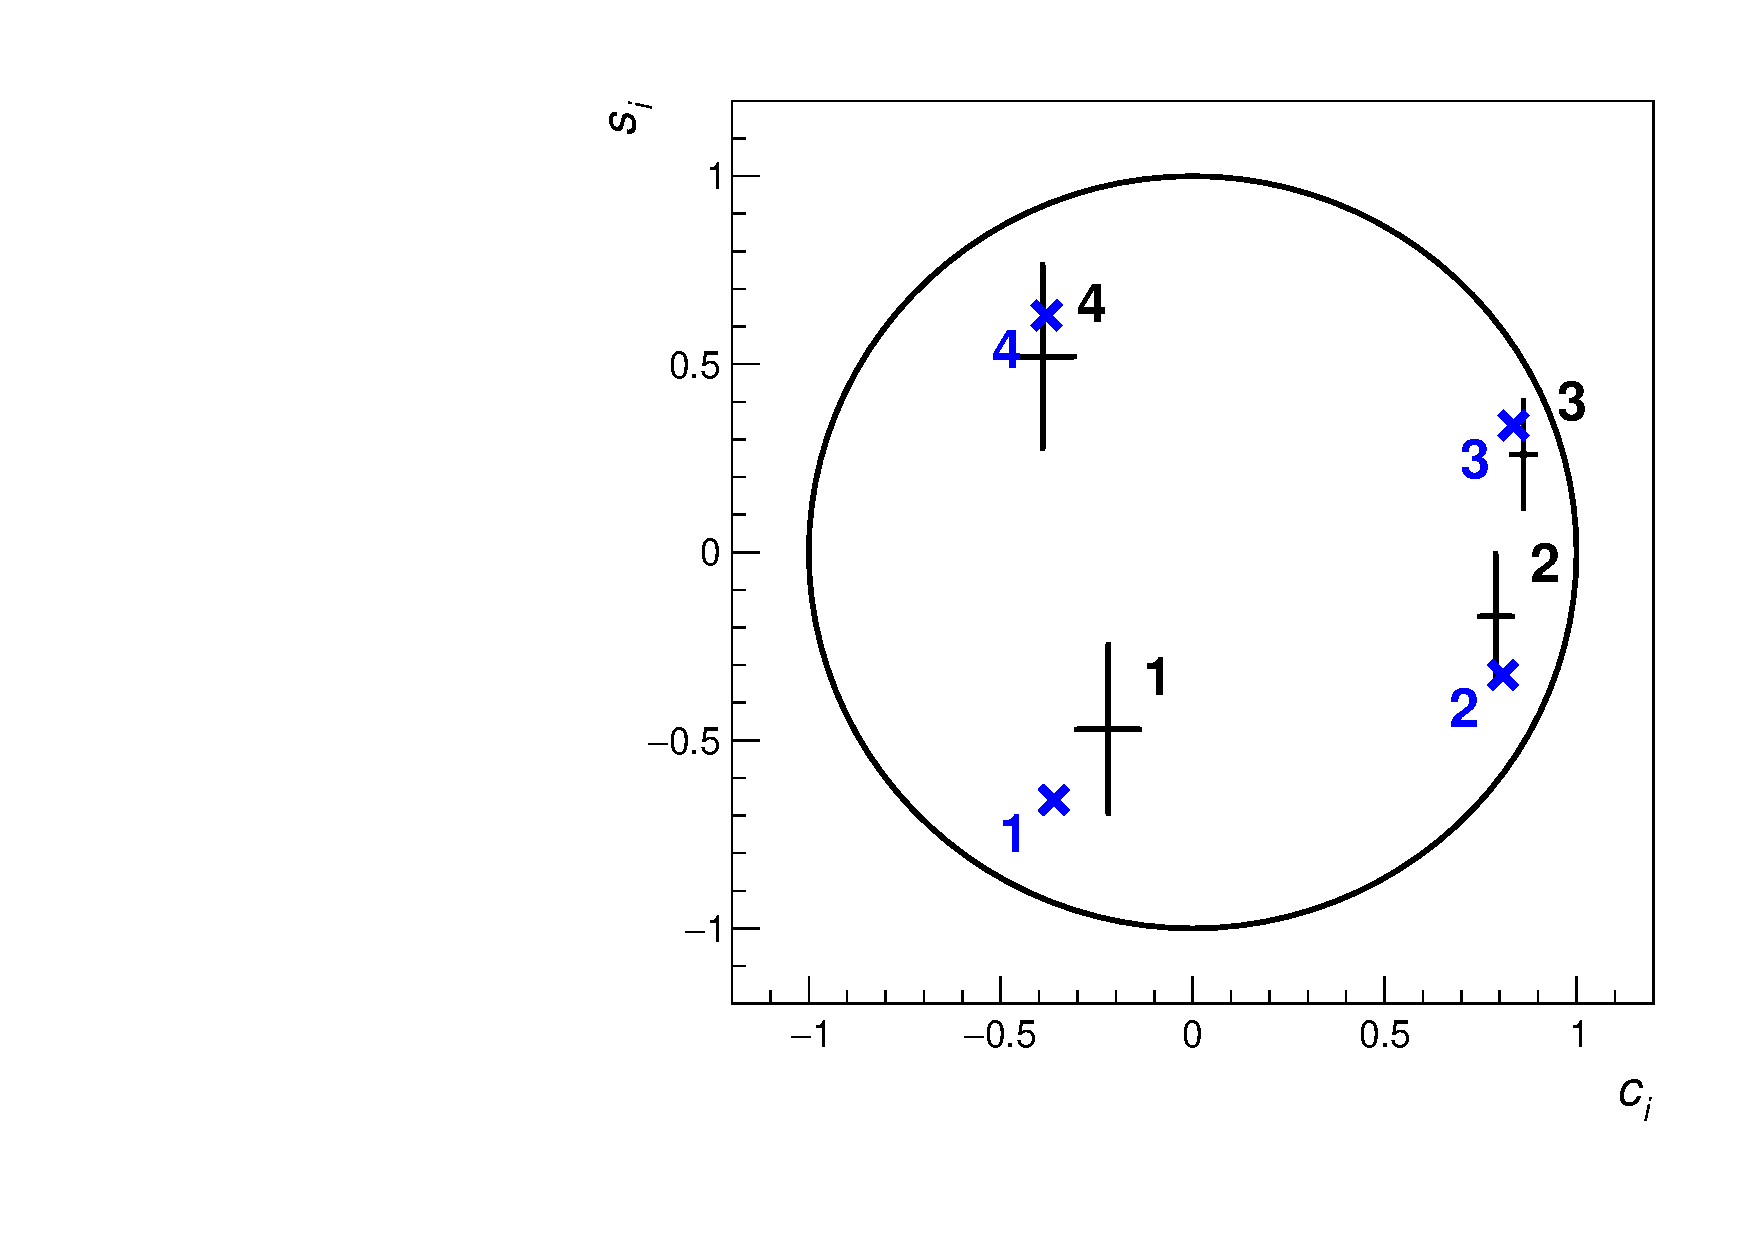
\includegraphics[width=0.9\textwidth]{Plots/cisi_FitResults_Model.pdf}
      \end{figure}
    \end{column}
  \end{columns}
  \begin{center}
    Measured values (black) are consistent and close to LHCb model predictions (blue), so central values are not expected to change much
  \end{center}
\end{frame}

\begin{frame}{BESIII preliminary $D^0\to\pi^+\pi^-\pi^+\pi^-$ strong-phase results}
  \begin{center}
    Small differences between model prediction and measurement, but data points are generally close to the unit circle
  \end{center}
  \vspace{-0.3cm}
  \begin{columns}
    \begin{column}{0.50\textwidth}
      \vspace{-0.5cm}
      \begin{align*}
        c_1 =& +0.12 \pm 0.09 \pm 0.02 \\
        s_1 =& -0.42 \pm 0.21 \pm 0.04 \\
        c_2 =& +0.74 \pm 0.04 \pm 0.02 \\
        s_2 =& -0.39 \pm 0.16 \pm 0.06 \\
        s_3 =& -0.25 \pm 0.12 \pm 0.03 \\
        c_3 =& +0.81 \pm 0.03 \pm 0.01 \\
        c_4 =& +0.42 \pm 0.06 \pm 0.02 \\
        s_4 =& +0.86 \pm 0.19 \pm 0.07 \\
        c_5 =& -0.27 \pm 0.09 \pm 0.03 \\
        s_5 =& -0.22 \pm 0.25 \pm 0.08
      \end{align*}
    \end{column}
    \begin{column}{0.50\textwidth}
      \begin{figure}
        \centering
        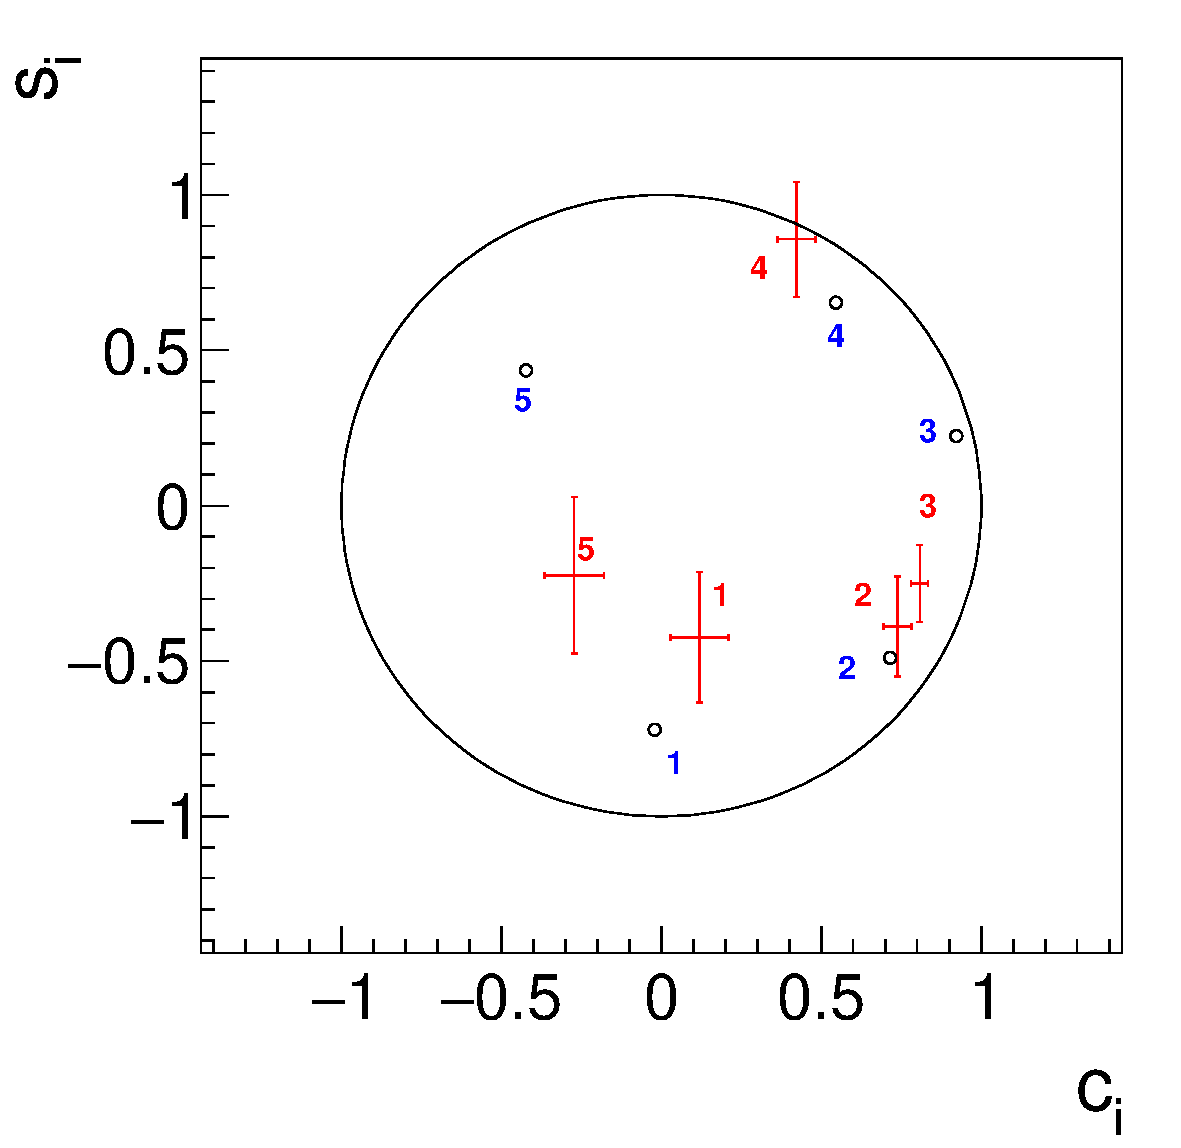
\includegraphics[width=1.0\textwidth]{Plots/CiSiOptim.pdf}
      \end{figure}
    \end{column}
  \end{columns}
  \begin{center}
    The HyperPlot software is used (binary lookup tree in 5D phase space)
  \end{center}
\end{frame}

\section{Analysis: Global fit}
\begin{frame}{Global fit}
  \begin{center}
    {\large Global fit of $K^+K^-\pi^+\pi^-$ remains as in model-dependent publication:}
  \end{center}
  \vspace{-0.5cm}
  \begin{figure}
    \centering
    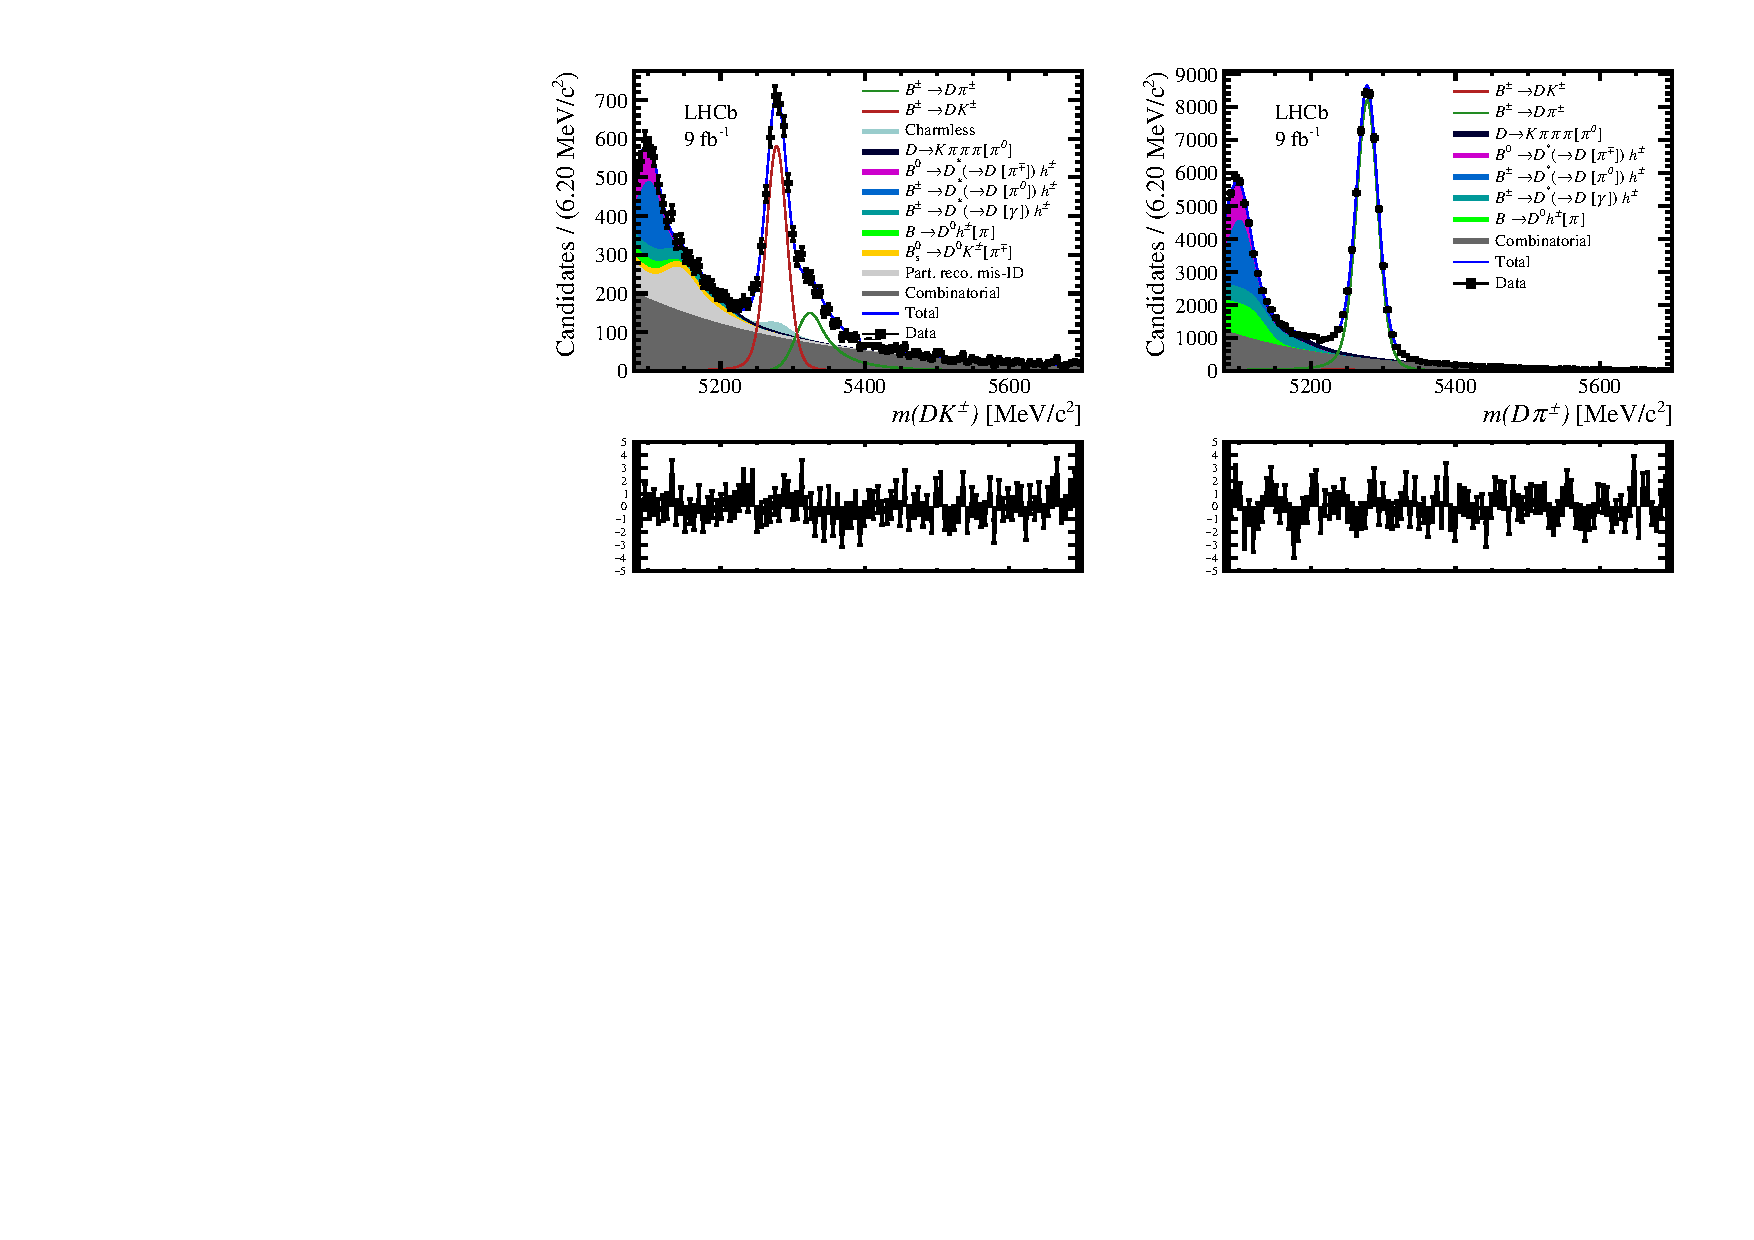
\includegraphics[width = 0.9\textwidth,trim={0 0 0 0},clip=true]{Plots/d2kkpipi_fiveL_allDP.pdf}
  \end{figure}
  \vspace{-0.5cm}
  \begin{itemize}
    \item{$B^\pm\to[K^+K^-\pi^+\pi^-]_Dh^\pm$ signal yield:}
    \begin{itemize}
      \item{$B^\pm\to DK^\pm$: $3280 \pm 41$}
      \item{$B^\pm\to D\pi^\pm$: $47610 \pm 231$}
    \end{itemize}
  \end{itemize}
\end{frame}

\begin{frame}{Global fit}
  \begin{center}
    {\large Global fit of $\pi^+\pi^-\pi^+\pi^-$ has a good fit quality:}
  \end{center}
  \vspace{-0.5cm}
  \begin{figure}
    \centering
    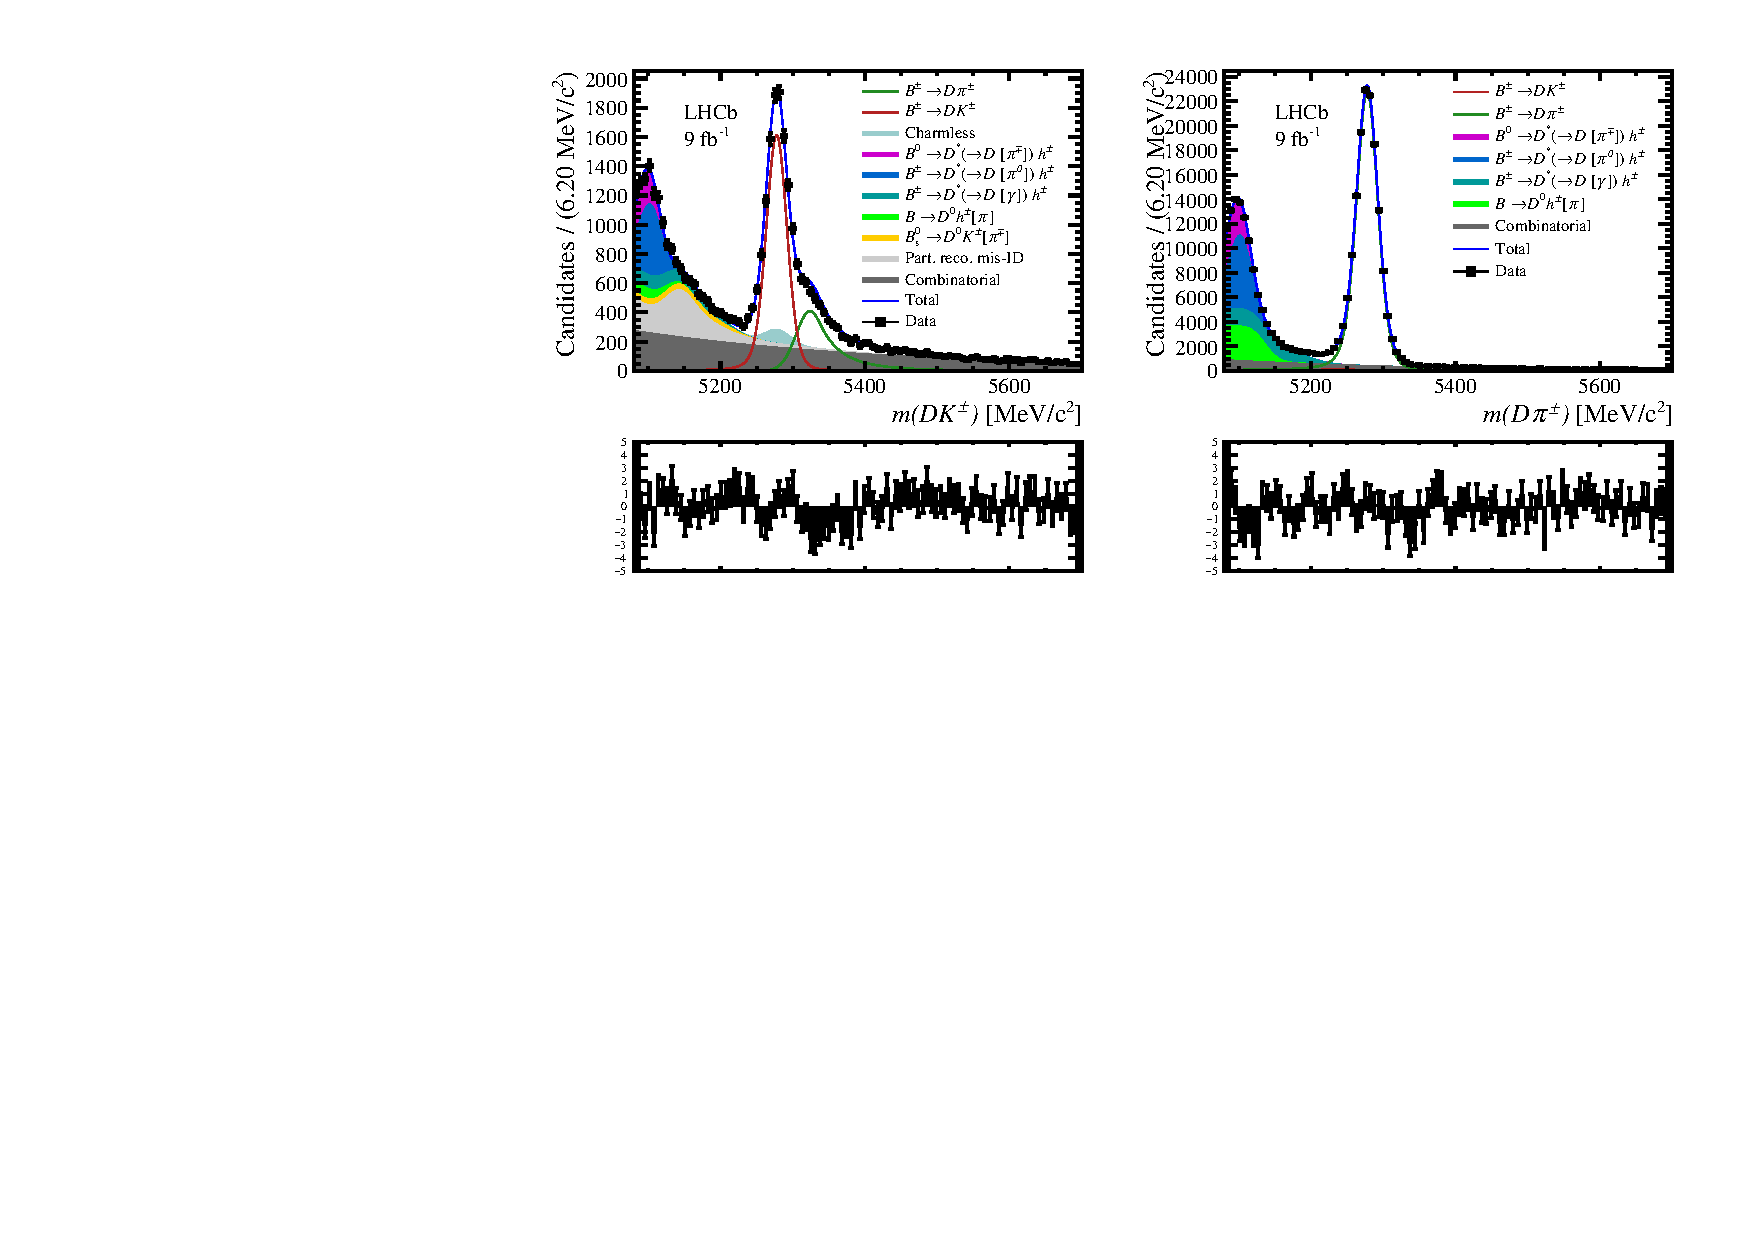
\includegraphics[width = 0.9\textwidth,trim={0 0 0 0},clip=true]{Plots/d2pipipipi_fiveL_allDP.pdf}
  \end{figure}
  \vspace{-0.5cm}
  \begin{itemize}
    \item{$B^\pm\to[\pi^+\pi^-\pi^+\pi^-]_Dh^\pm$ signal yield:}
    \begin{itemize}
      \item{$B^\pm\to DK^\pm$: $9172 \pm 110$}
      \item{$B^\pm\to D\pi^\pm$: $132246 \pm 394$}
    \end{itemize}
  \end{itemize}
\end{frame}

\section{Analysis: CP fit}
\begin{frame}{CP fit}
  \begin{center}
    {\large After global fit, perform a ``CP fit'' to study CP violation:}
  \end{center}
  \begin{itemize}
    \setlength\itemsep{1.0em}
    \item{Split candidates by:}
    \begin{enumerate}
      \item{$B^+$ and $B^-$ charges}
      \item{$B^\pm\to DK^\pm$ and $B^\pm\to D\pi^\pm$ decays}
      \item{$D$ phase-space bins}
    \end{enumerate}
    \item{Combinatorial and low-mass backgrounds are floating in each category}
    \item{Parameterise signal yields in terms of $x_\pm^{DK}$, $y_\pm^{DK}$, $x_\xi^{D\pi}$, $y_\xi^{D\pi}$}
    \item{$2N - 1$ floating $F_i$ parameters}
    \item{\underline{$c_i$ and $s_i$ are Gaussian constrained}}
  \end{itemize}
\end{frame}

\begin{frame}{CP fit bin asymmetry}
  \begin{center}
    {\large Example of bin asymmetry in $D\to K^+K^-\pi^+\pi^-$ bin $-3$:}
  \end{center}
  \begin{figure}
    \centering
    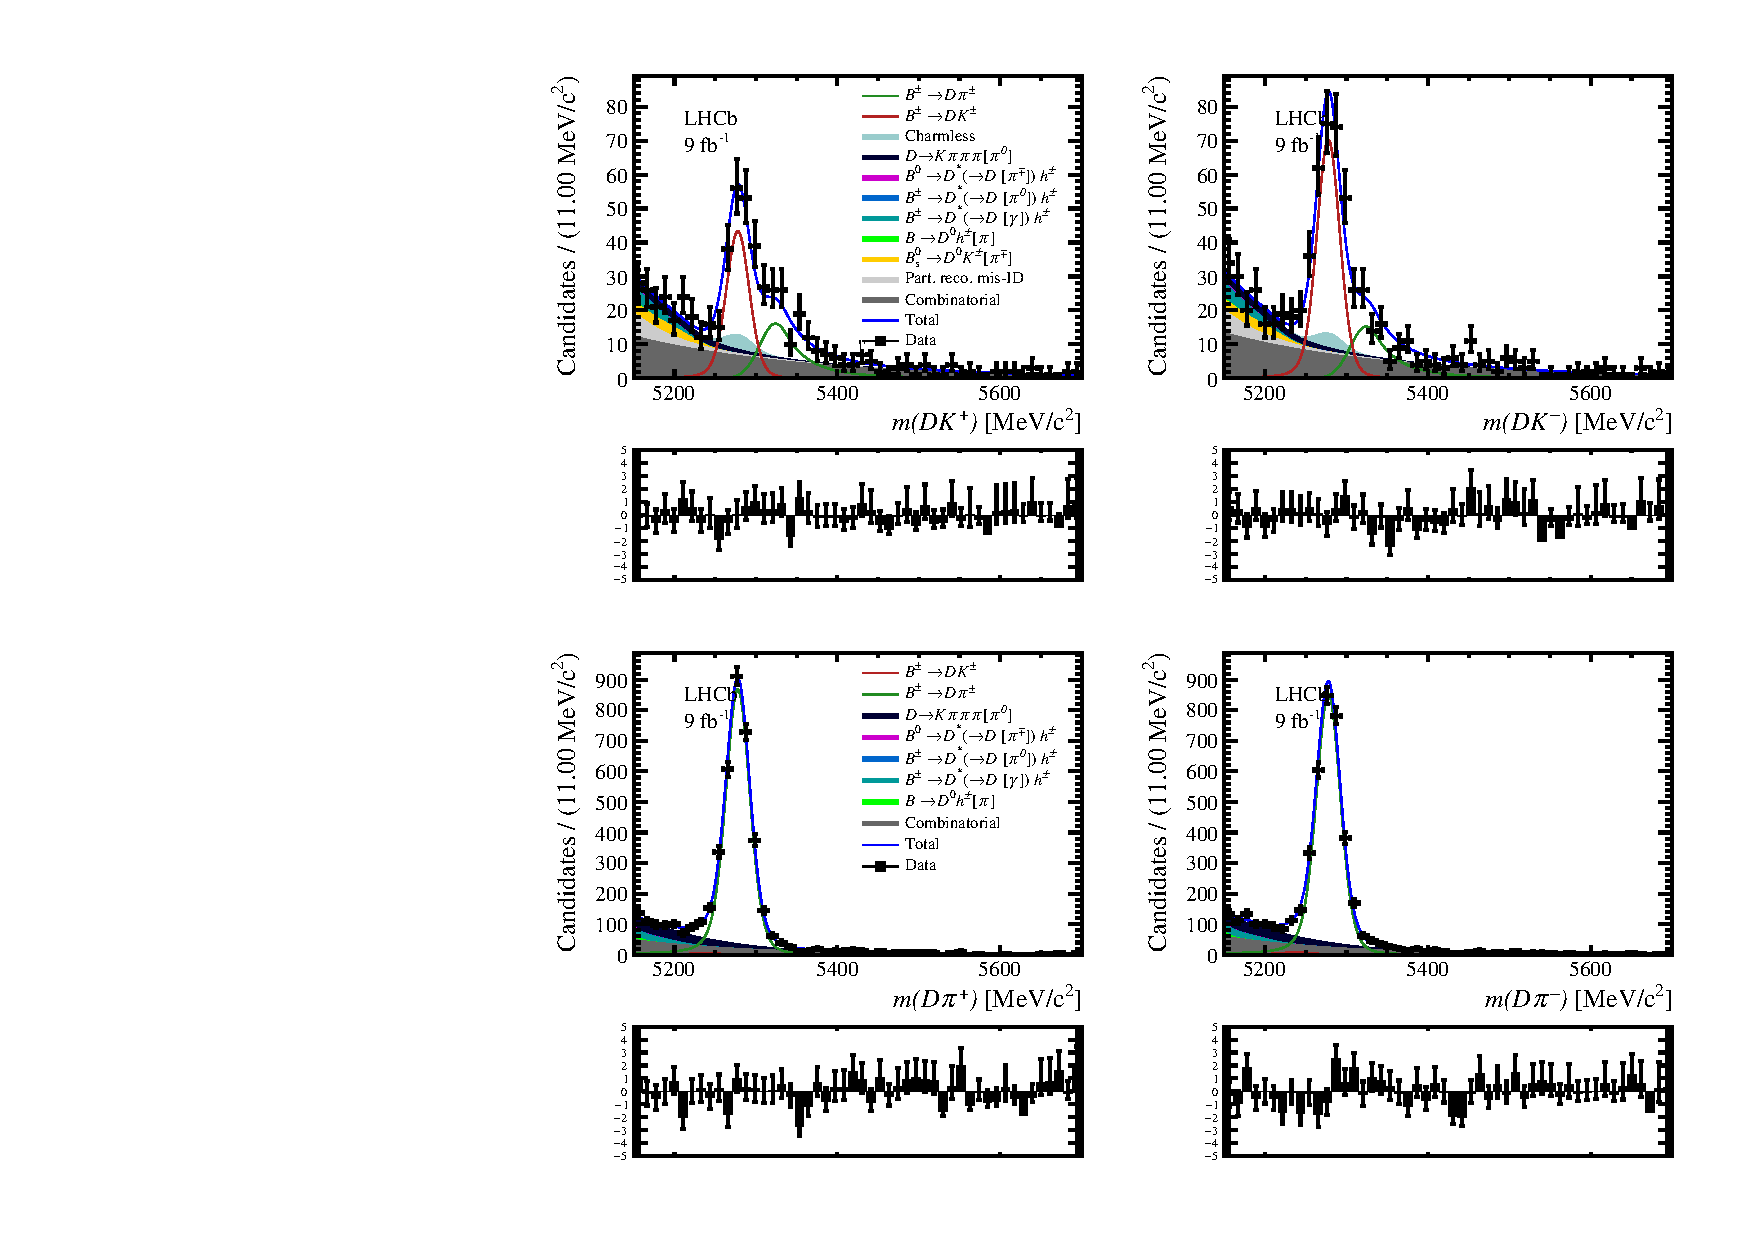
\includegraphics[width = 0.9\textwidth,trim={0 10cm 0 0},clip=true]{Plots/d2kkpipi_fiveL_binm3.pdf}
  \end{figure}
\end{frame}

\begin{frame}{CP fit bin asymmetry}
  \begin{center}
    {\large Example of bin asymmetry in $D\to\pi^+\pi^-\pi^+\pi^-$ bin $+5$:}
  \end{center}
  \begin{figure}
    \centering
    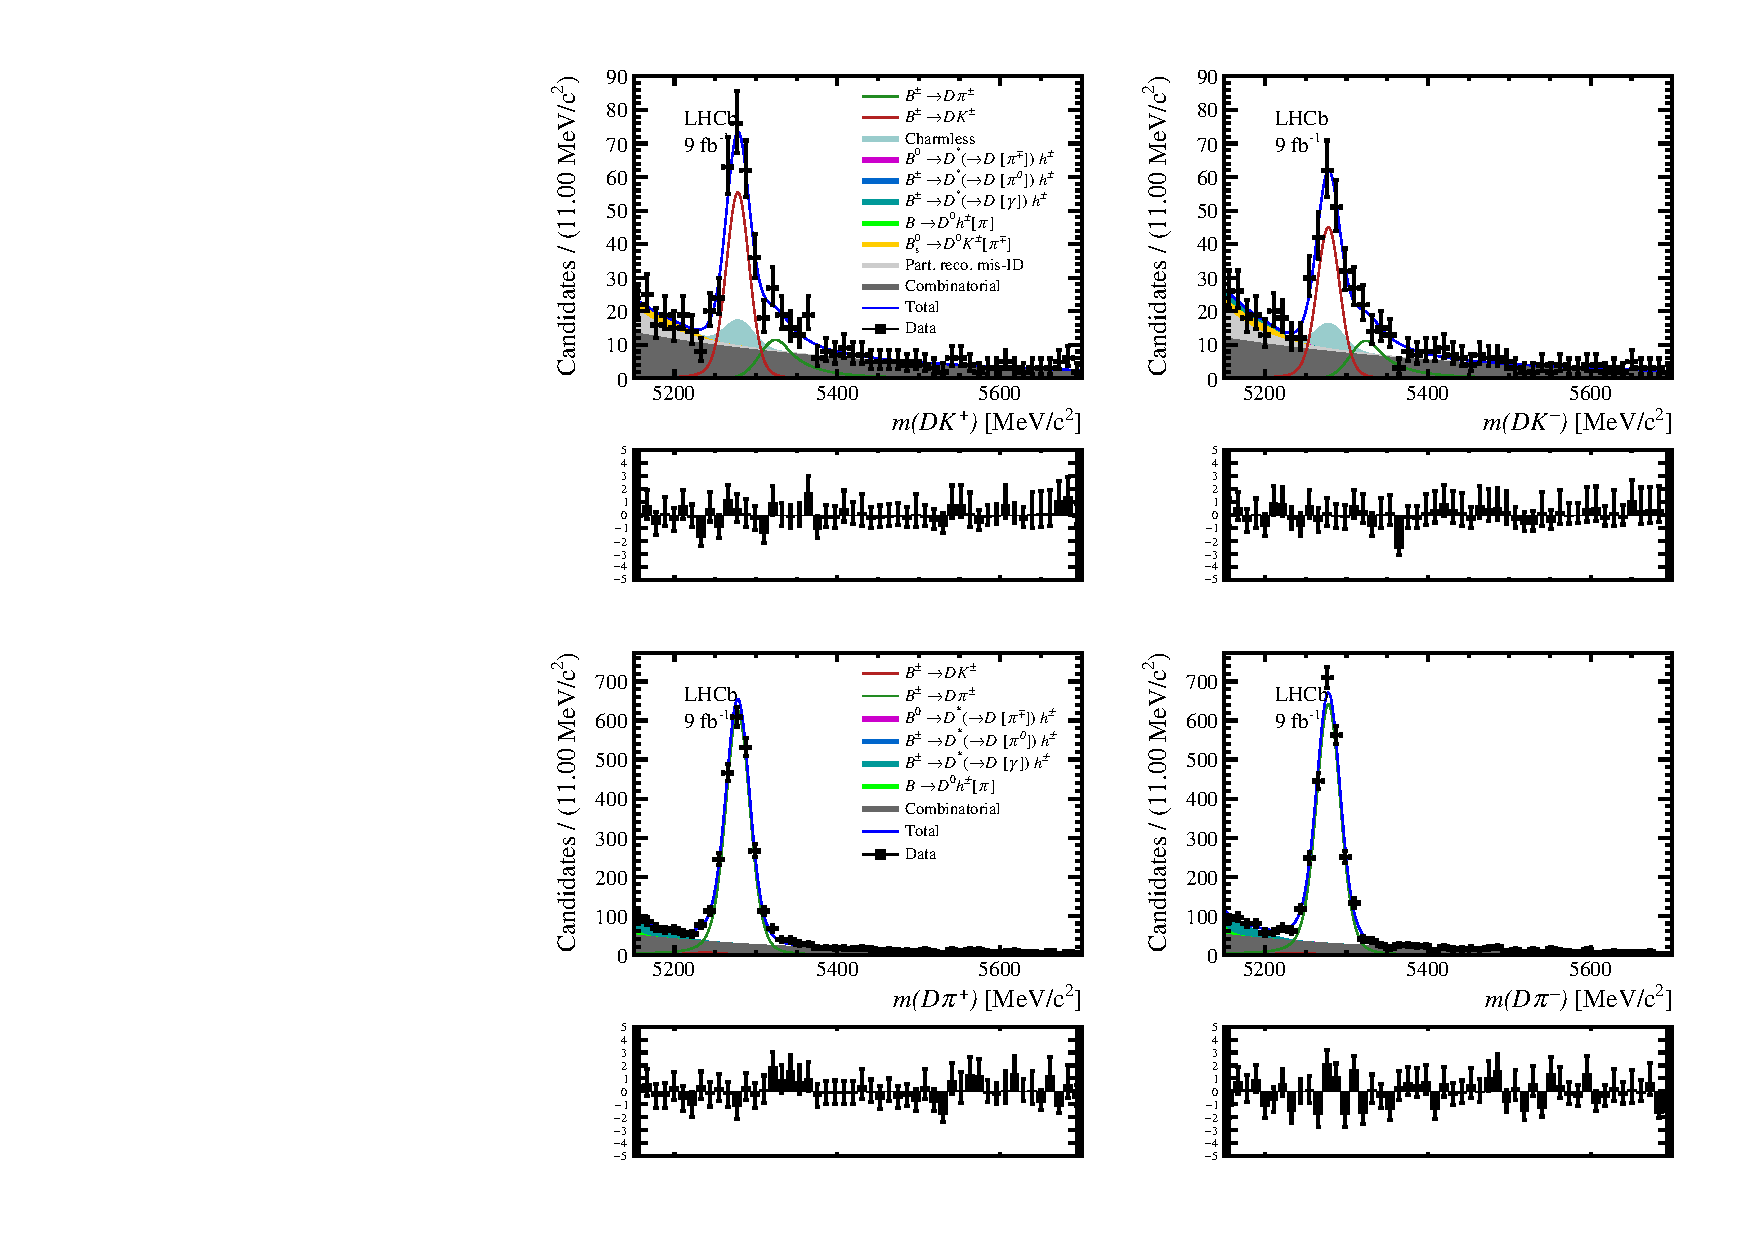
\includegraphics[width = 0.9\textwidth,trim={0 10cm 0 0},clip=true]{Plots/d2pipipipi_fiveL_binp5.pdf}
  \end{figure}
\end{frame}

\begin{frame}{Bin asymmetries}
  \begin{center}
    $B^\pm\to[K^+K^-\pi^+\pi^-]_Dh^\pm$ bin asymmetries
  \end{center}
  \begin{figure}
    \centering
    \begin{subfigure}{0.5\textwidth}
      \centering
      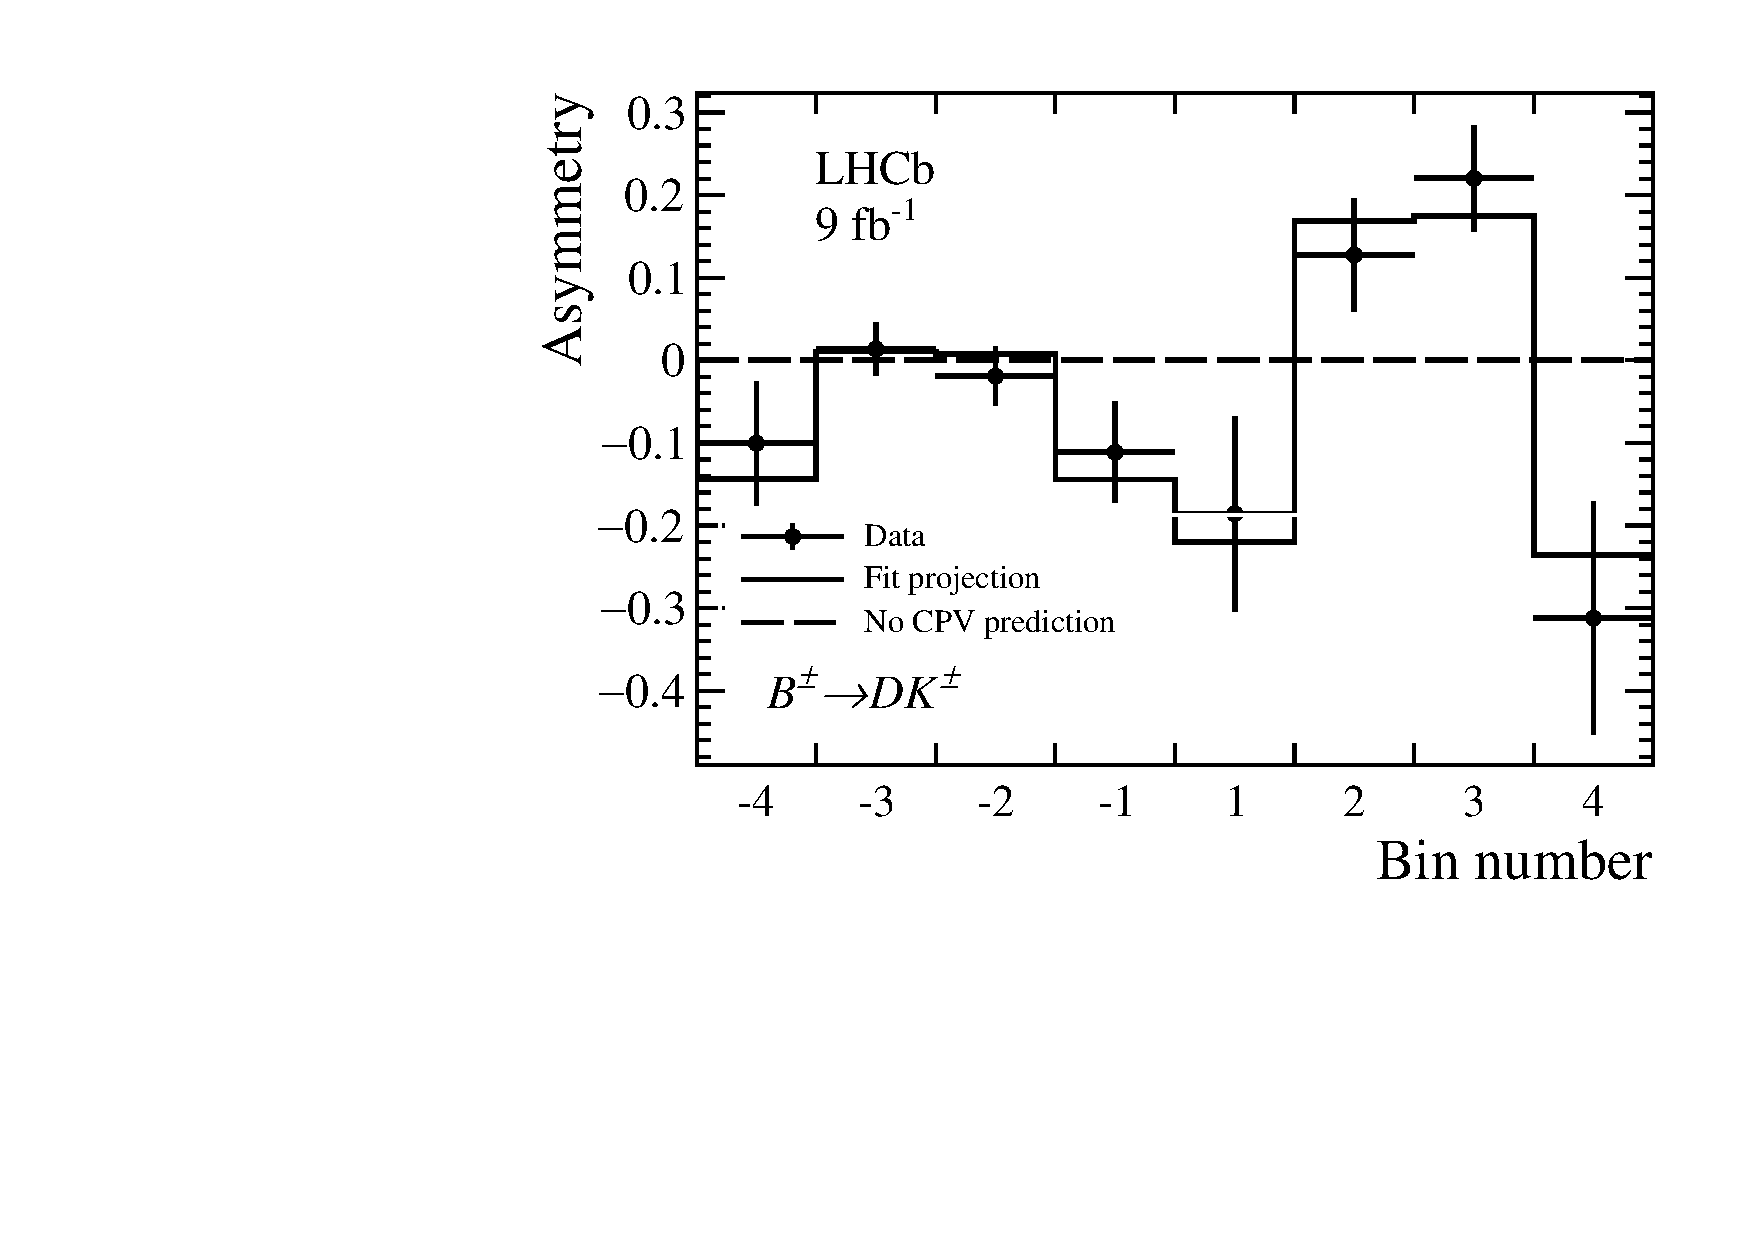
\includegraphics[width=1.0\textwidth]{Plots/BinAsymmetries_dk_KKpipi.pdf}
      \caption*{$B^\pm\to DK^\pm$}
    \end{subfigure}%
    \begin{subfigure}{0.5\textwidth}
      \centering
      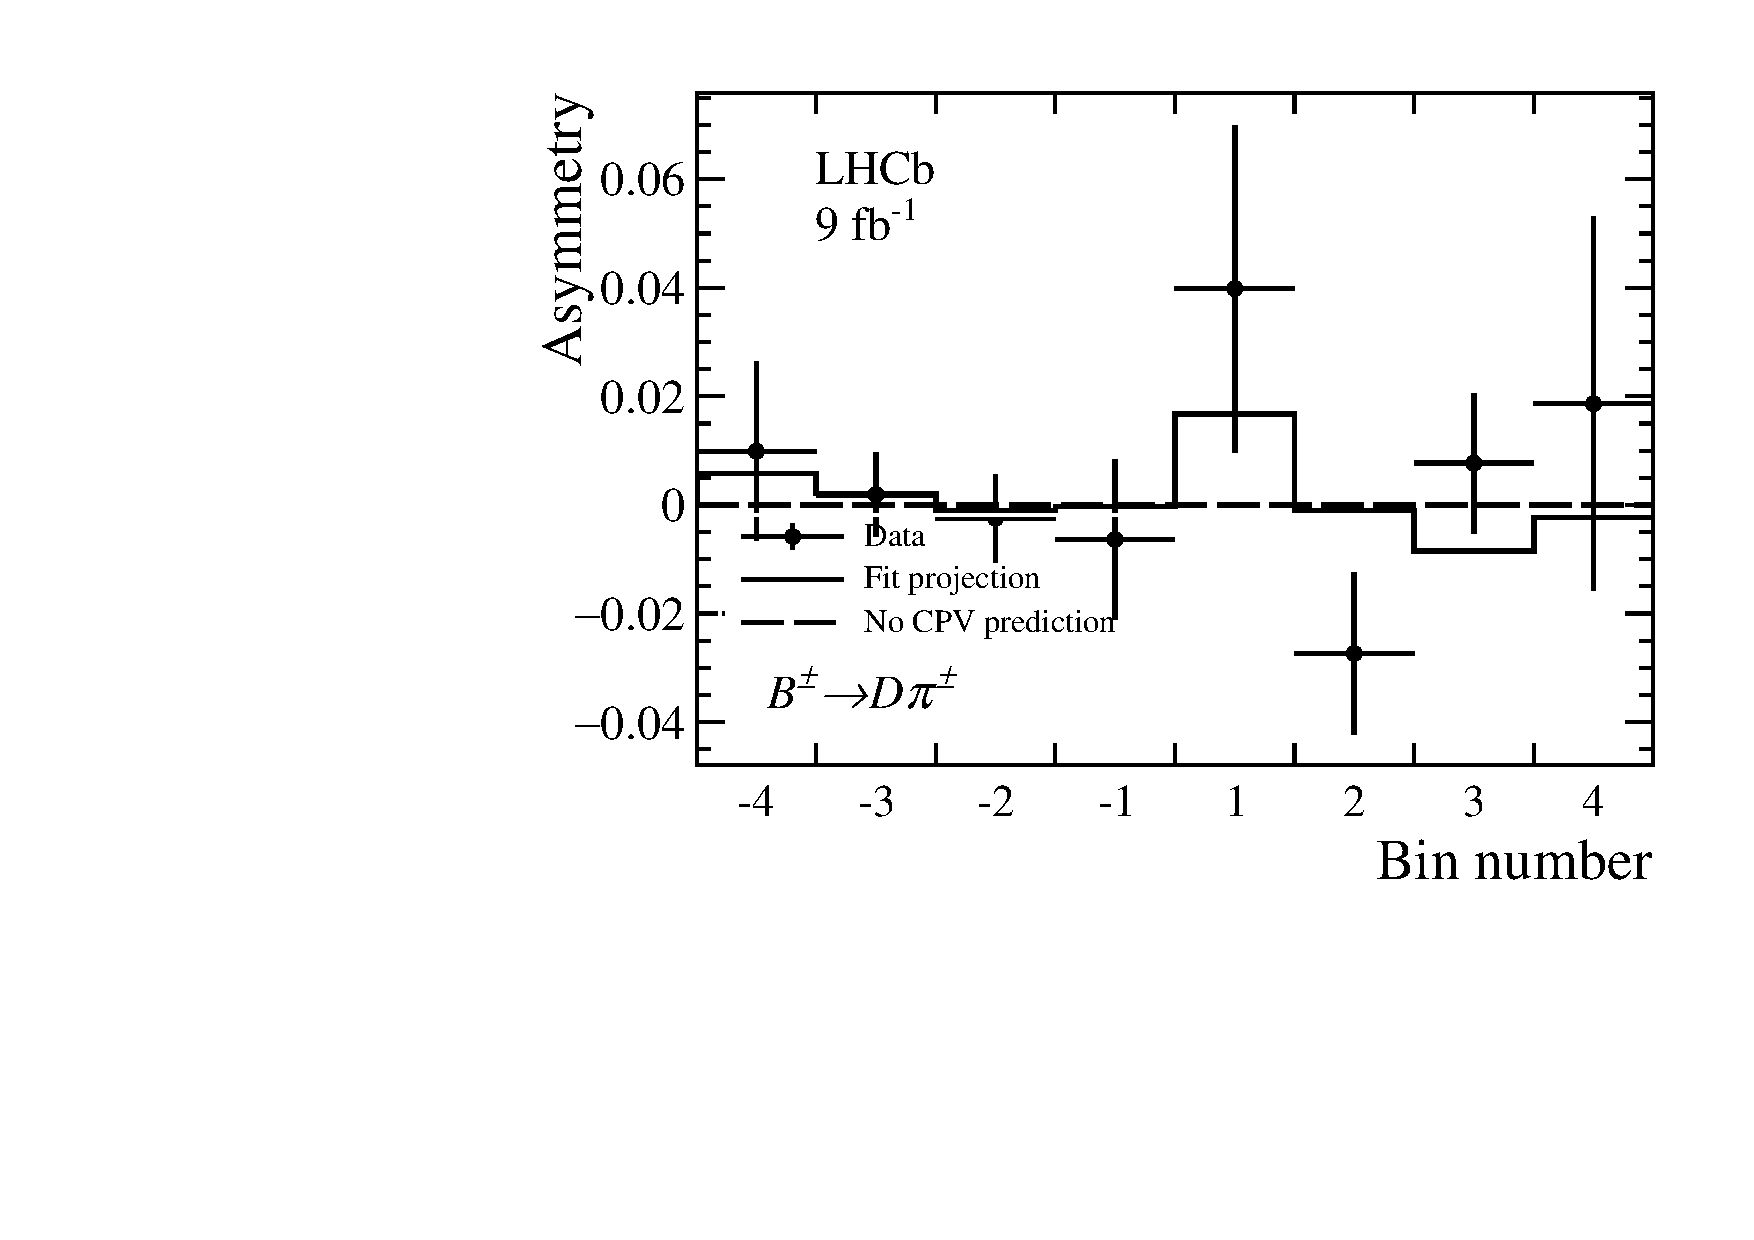
\includegraphics[width=1.0\textwidth]{Plots/BinAsymmetries_dpi_KKpipi.pdf}
      \caption*{$B^\pm\to D\pi^\pm$}
    \end{subfigure}
  \end{figure}
\end{frame}

\begin{frame}{Bin asymmetries}
  \begin{center}
    $B^\pm\to[\pi^+\pi^-\pi^+\pi^-]_Dh^\pm$ bin asymmetries
  \end{center}
  \begin{figure}
    \centering
    \begin{subfigure}{0.5\textwidth}
      \centering
      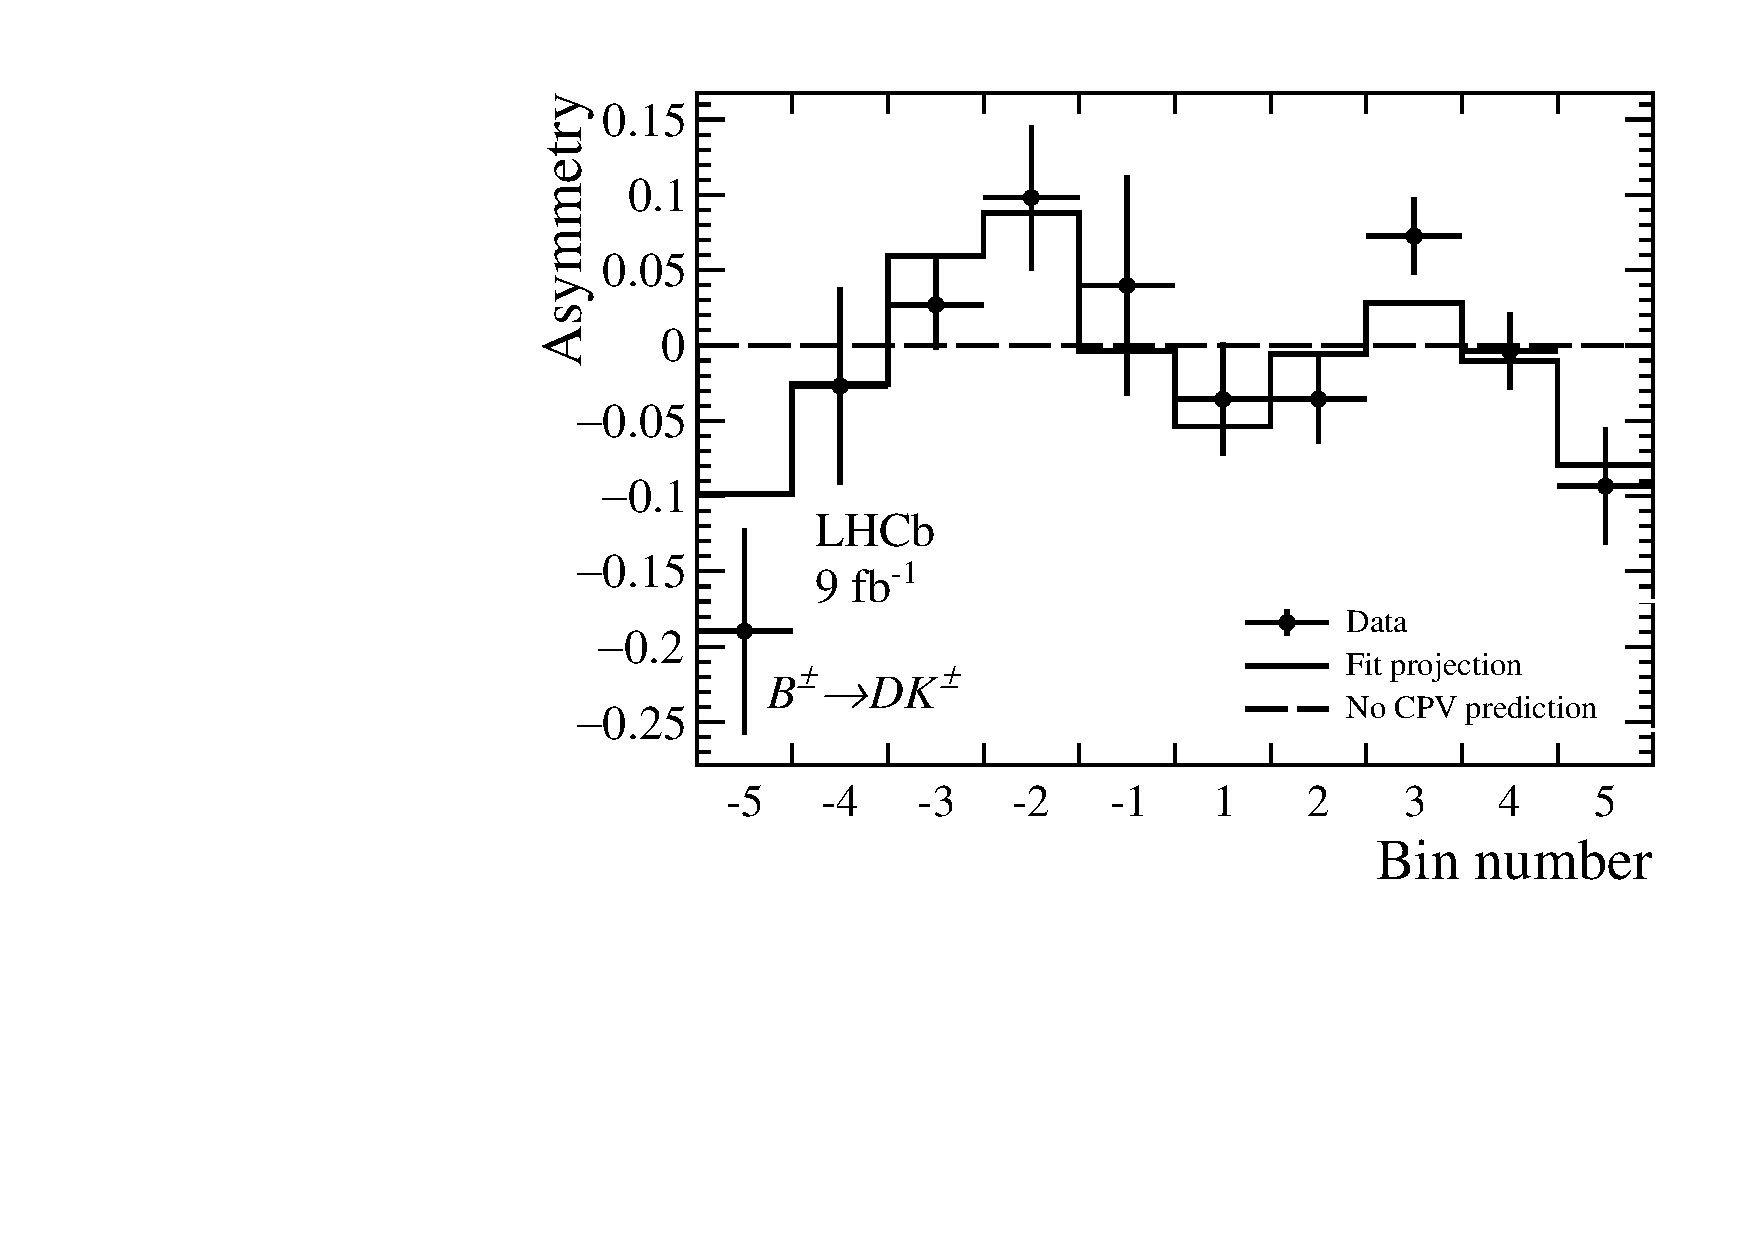
\includegraphics[width=1.0\textwidth]{Plots/BinAsymmetries_dk_pipipipi.pdf}
      \caption*{$B^\pm\to DK^\pm$}
    \end{subfigure}%
    \begin{subfigure}{0.5\textwidth}
      \centering
      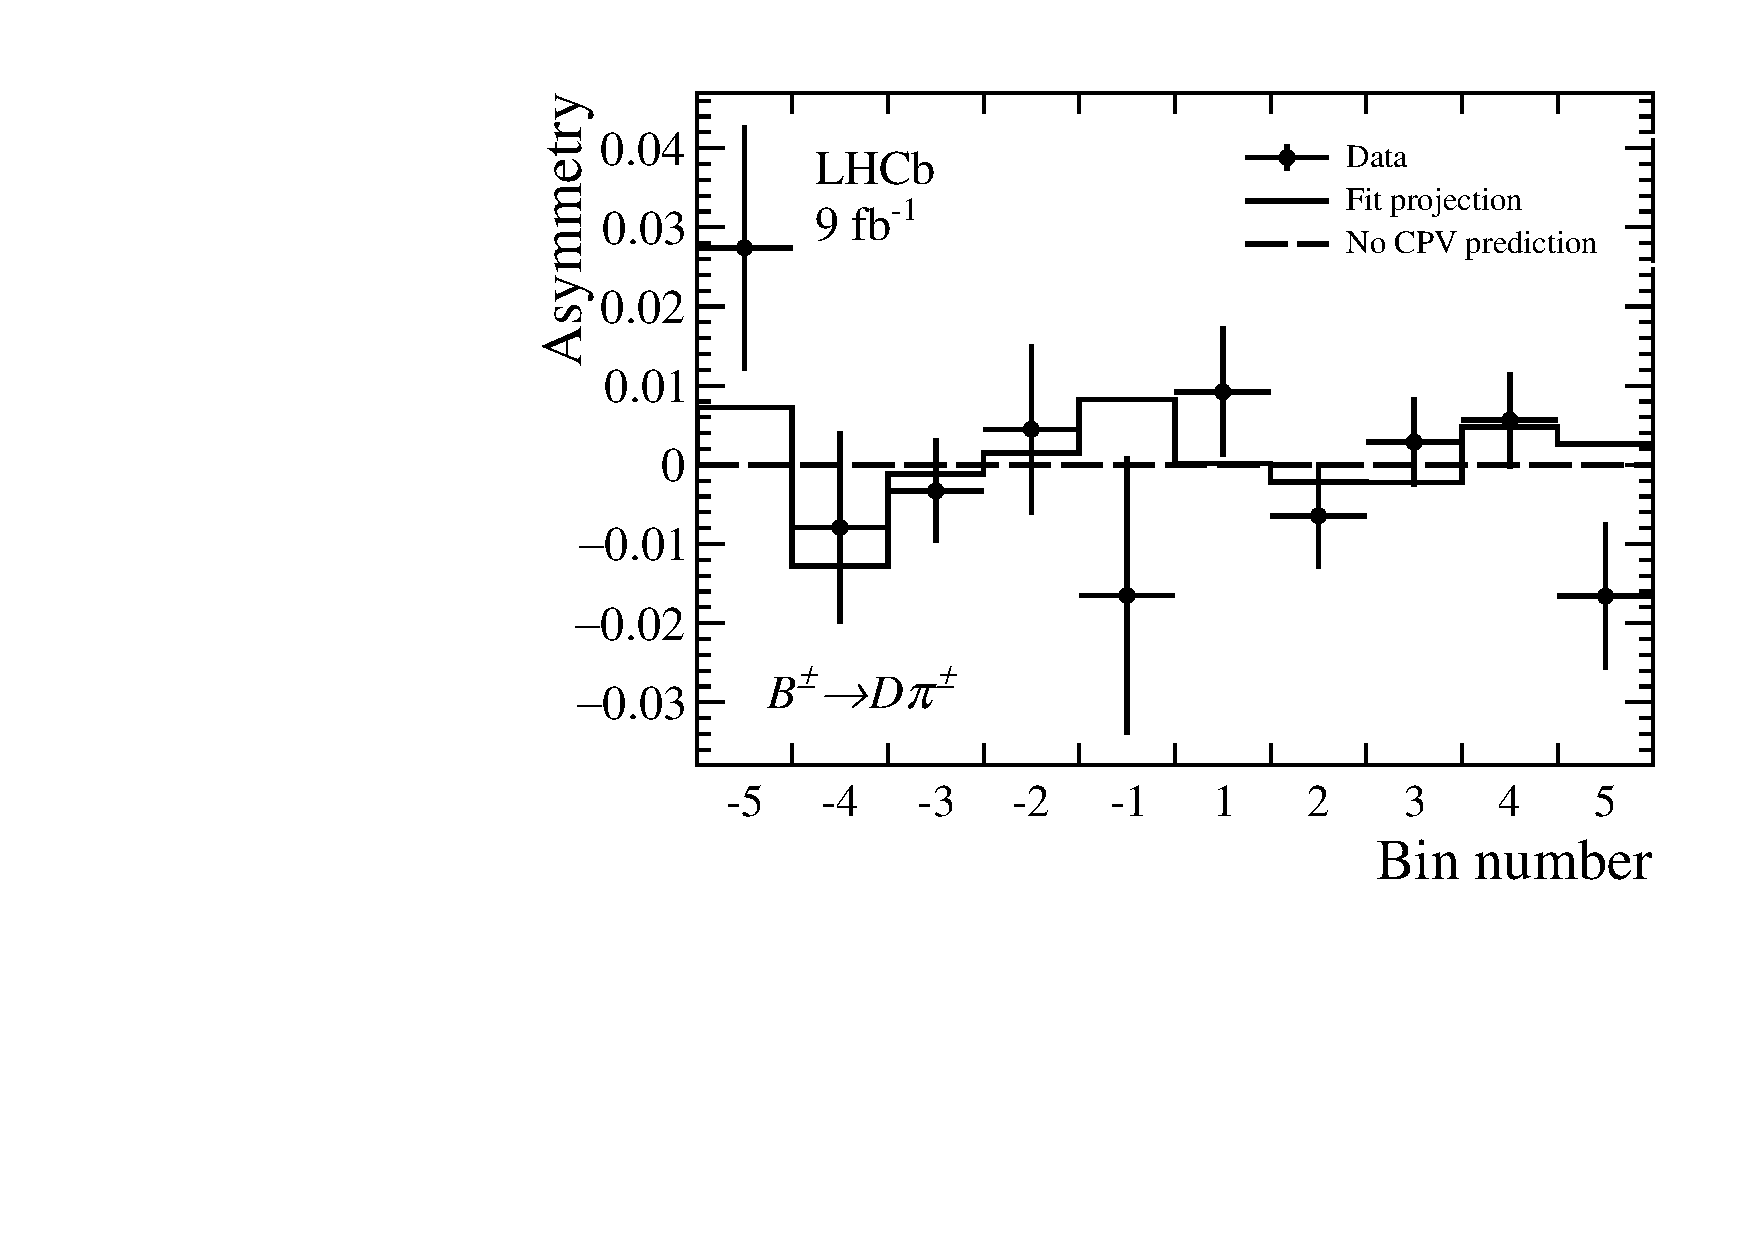
\includegraphics[width=1.0\textwidth]{Plots/BinAsymmetries_dpi_pipipipi.pdf}
      \caption*{$B^\pm\to D\pi^\pm$}
    \end{subfigure}
  \end{figure}
\end{frame}

\begin{frame}{Likelihood scan of CP observables}
  \begin{center}
    $x_\pm^{DK}$ agree well between likelihood scan and Hesse approximation
  \end{center}
  \begin{figure}
    \centering
    \begin{subfigure}{0.5\textwidth}
      \centering
      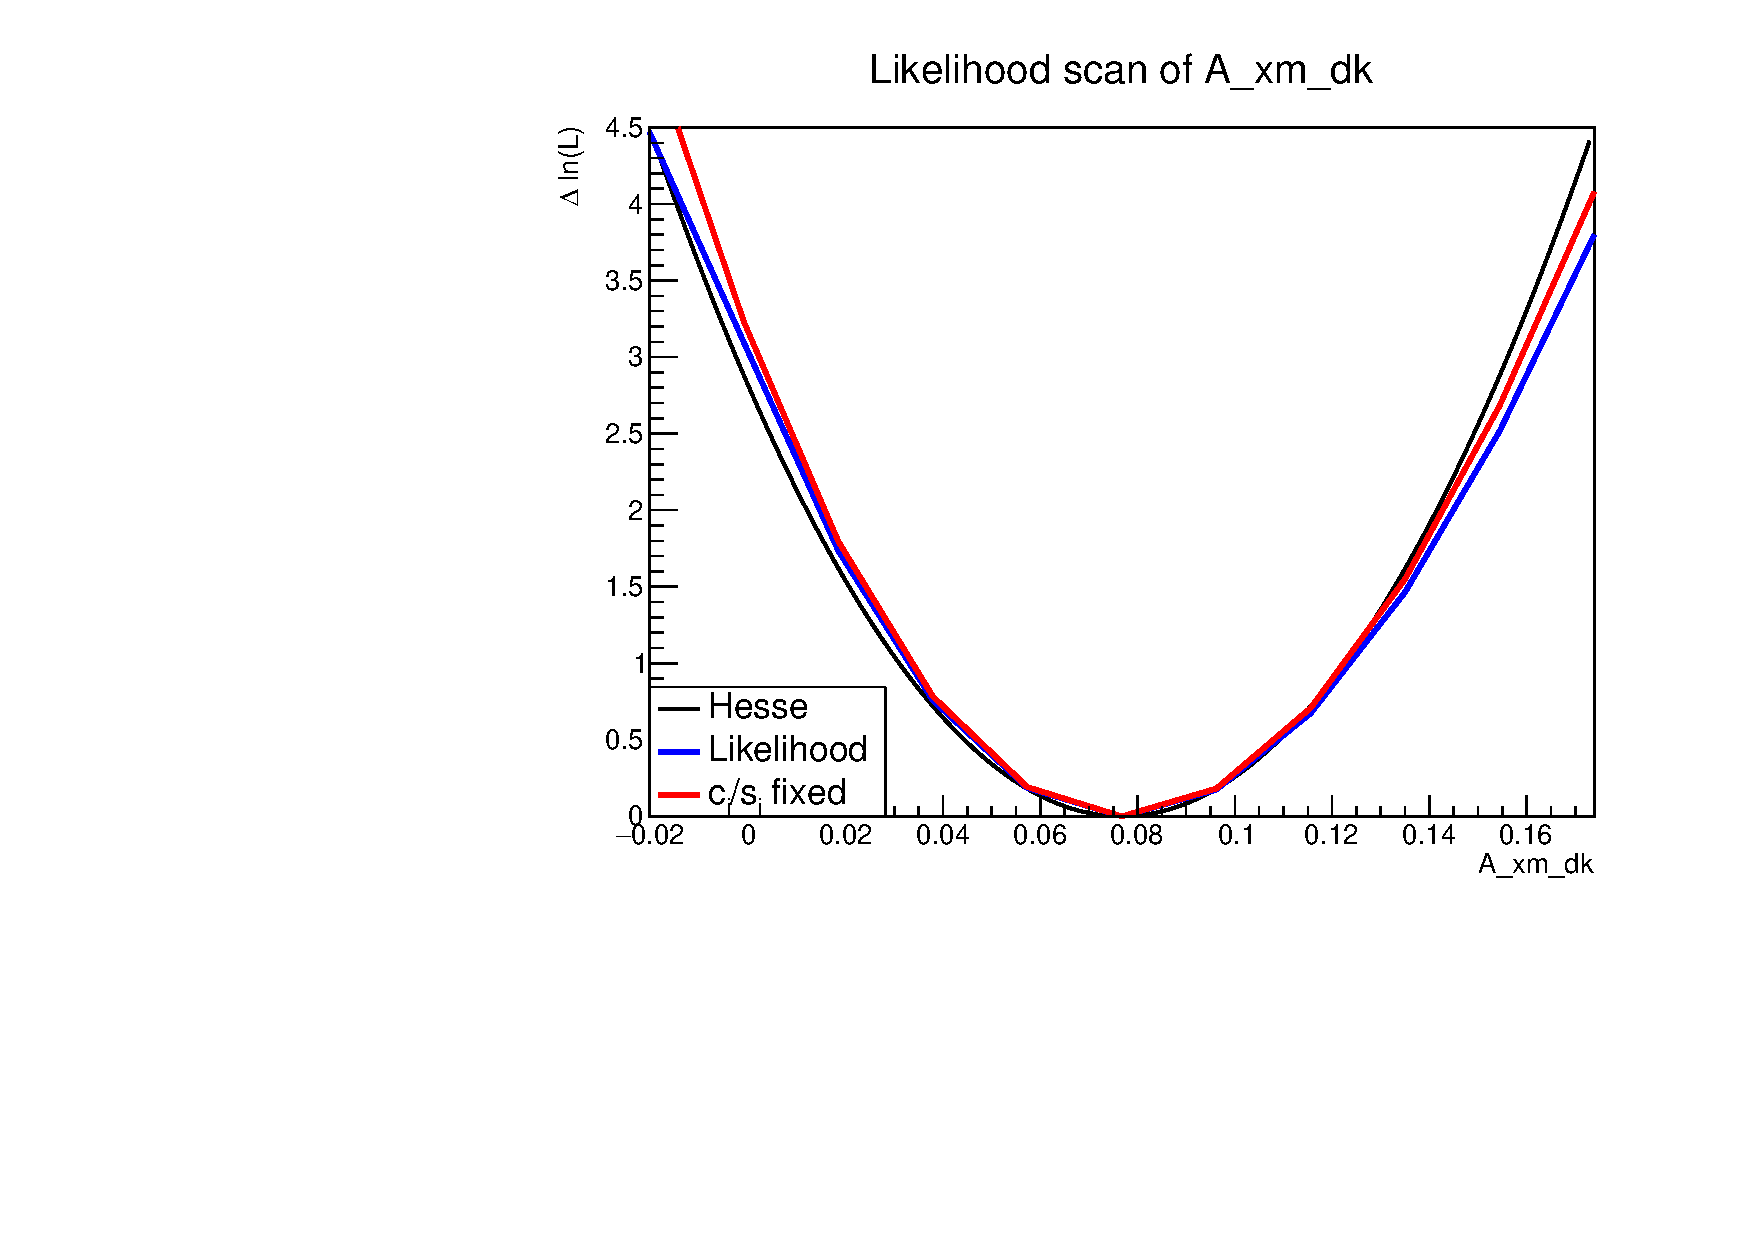
\includegraphics[width=1.0\textwidth]{Plots/A_xm_dk_likelihood_scan_KKpipi.pdf}
      \vspace{-0.3cm}
      \caption*{$x_-^{DK}$}
    \end{subfigure}%
    \begin{subfigure}{0.5\textwidth}
      \centering
      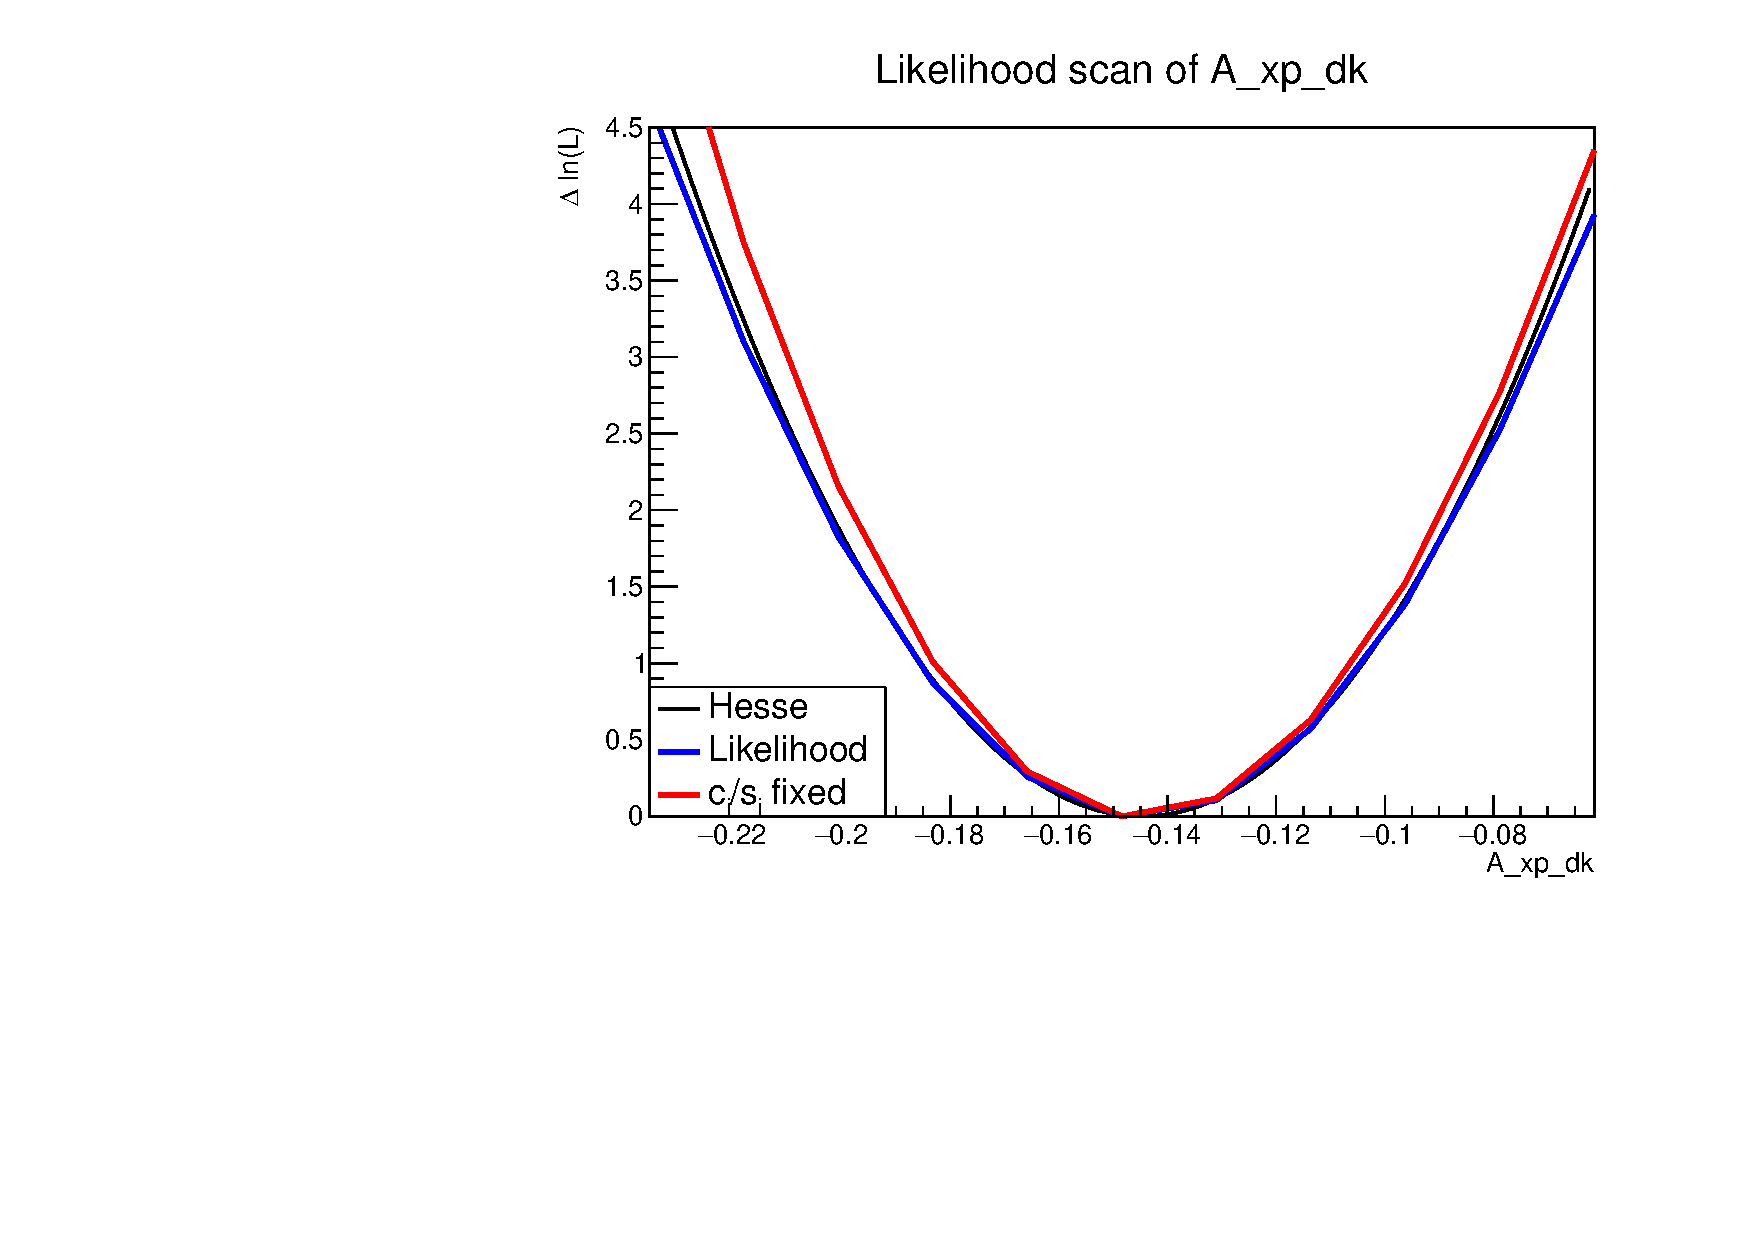
\includegraphics[width=1.0\textwidth]{Plots/A_xp_dk_likelihood_scan_KKpipi.pdf}
      \vspace{-0.3cm}
      \caption*{$x_+^{DK}$}
    \end{subfigure}
    \caption*{$D^0\to K^+K^-\pi^+\pi^-$}
  \end{figure}
\end{frame}

\begin{frame}{Likelihood scan of CP observables}
  \begin{center}
    $y_\pm^{DK}$ diverges from Hesse approximation outside $1\sigma$
  \end{center}
  \begin{figure}
    \centering
    \begin{subfigure}{0.5\textwidth}
      \centering
      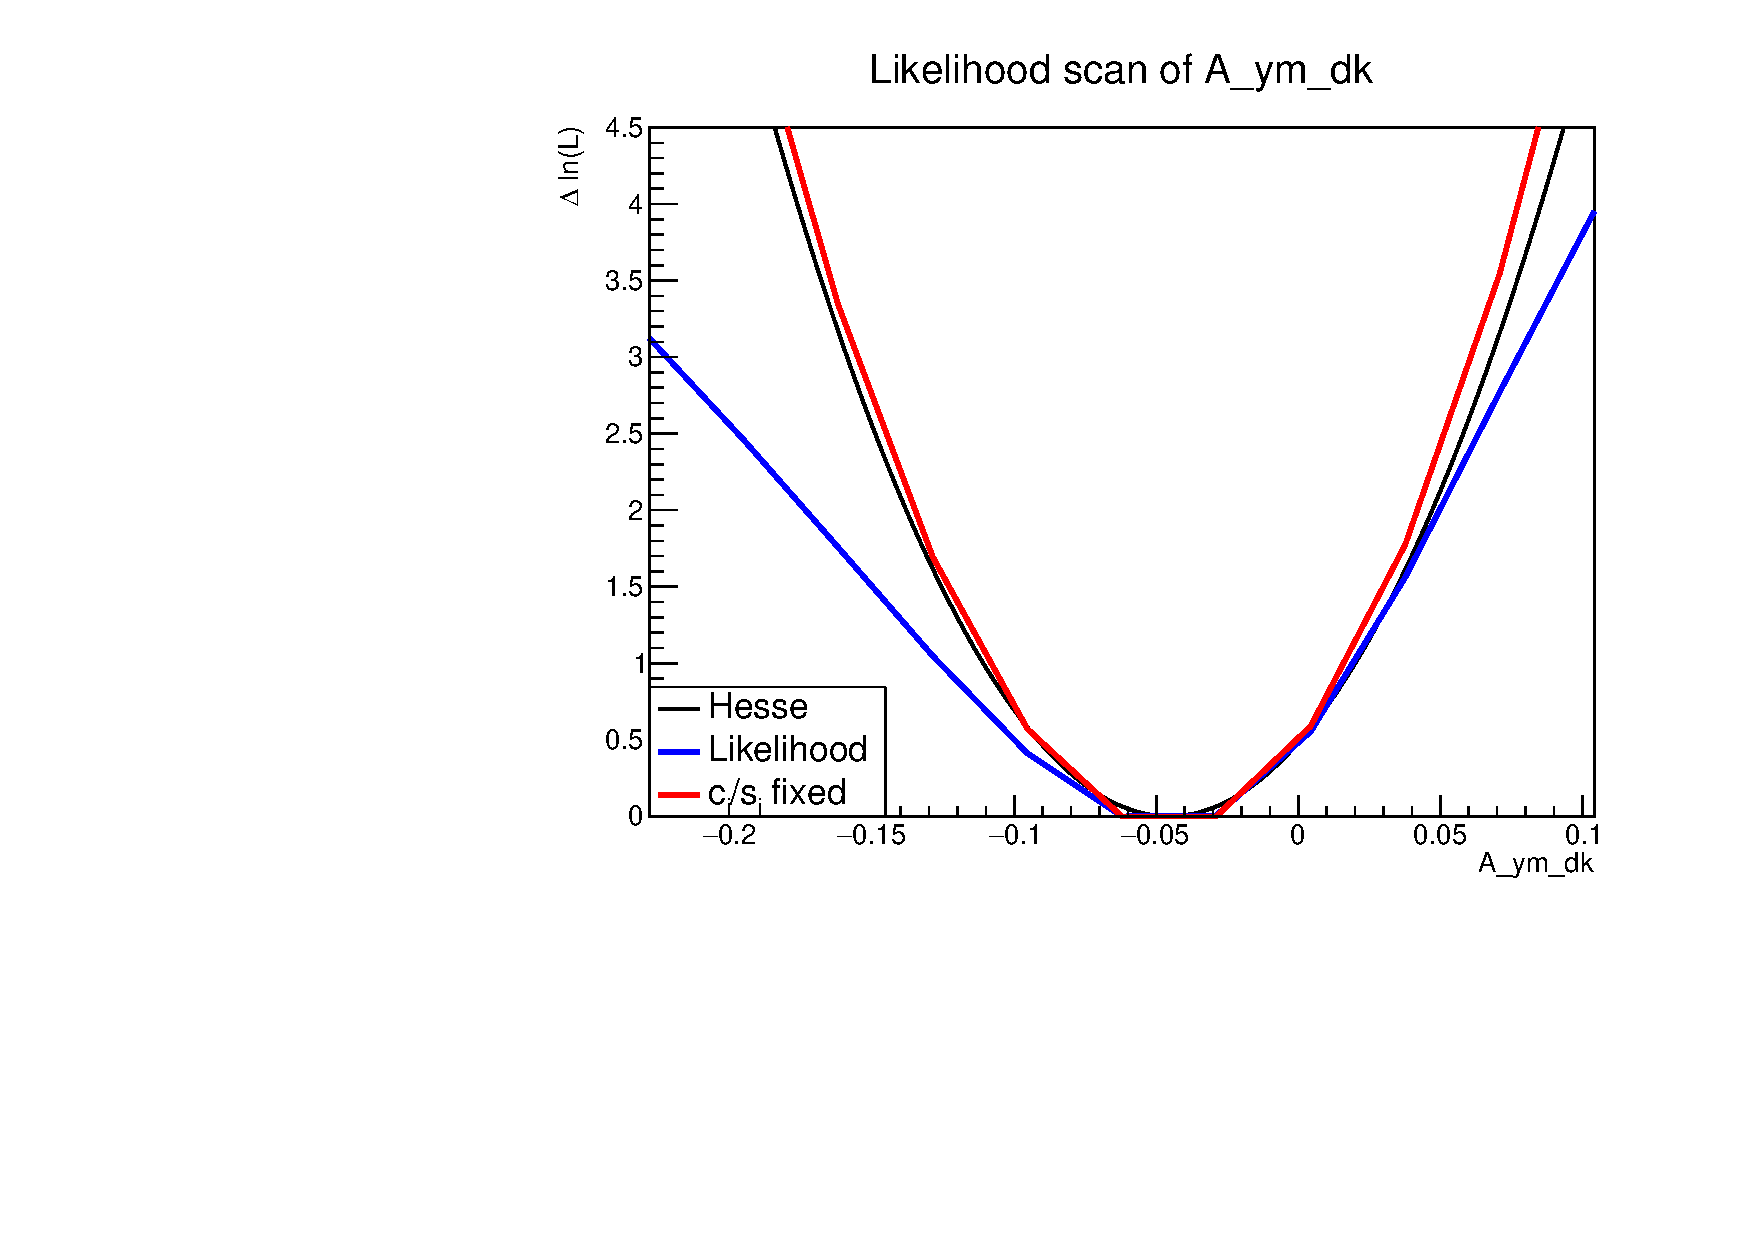
\includegraphics[width=1.0\textwidth]{Plots/A_ym_dk_likelihood_scan_KKpipi.pdf}
      \vspace{-0.3cm}
      \caption*{$y_-^{DK}$}
    \end{subfigure}%
    \begin{subfigure}{0.5\textwidth}
      \centering
      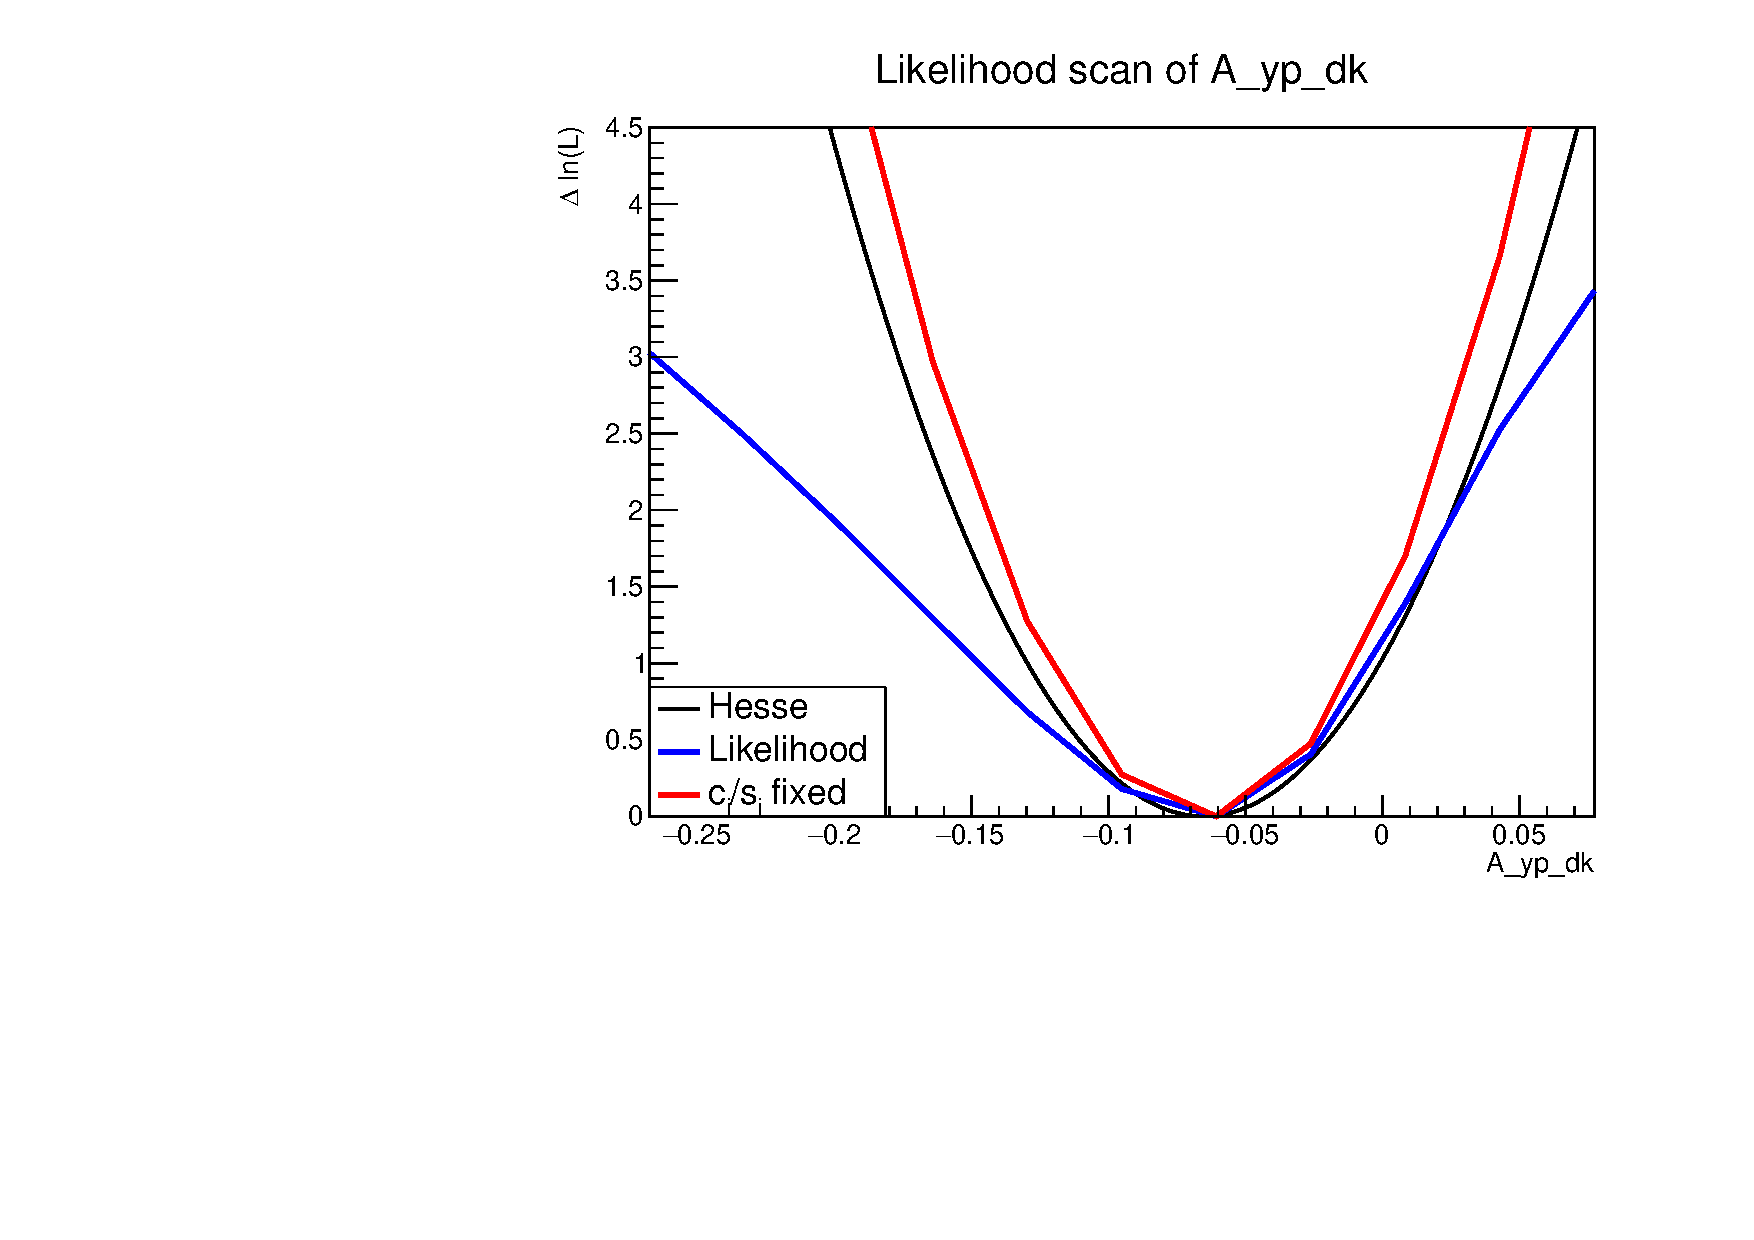
\includegraphics[width=1.0\textwidth]{Plots/A_yp_dk_likelihood_scan_KKpipi.pdf}
      \vspace{-0.3cm}
      \caption*{$y_+^{DK}$}
    \end{subfigure}
    \caption*{$D^0\to K^+K^-\pi^+\pi^-$}
  \end{figure}
\end{frame}

\begin{frame}{Likelihood scan of CP observables}
  \begin{center}
    {\large What do the likelihood scans tell us?}
  \end{center}
  \begin{itemize}
    \setlength\itemsep{1.5em}
    \item{Uncertainties from $c_i$ and $s_i$ are significant, which justifies Gaussian constraining $c_i$ and $s_i$}
    \item{New strategy:}
    \begin{enumerate}
      \setlength\itemsep{0.5em}
      \item{Produce a likelihood function from CP fit}
      \item{Interpret CP observables in terms of $\gamma$, etc}
      \item{Must \underline{profile} all nuisance parameters ($F_i$, $c_i$, $s_i$, backgrounds yields, normalisation constants)}
      \item{Provide direct measurements of $\gamma$, $\delta_B$ and $r_B$}
    \end{enumerate}
  \end{itemize}
\end{frame}

\begin{frame}{Summary of LHCb internal systematic uncertainties}
  \scriptsize
  \vspace{0.02cm}
  \begin{center}
    \begin{tabular}{lcccccc}
      \hline
      Source & $x_-^{DK}$ & $y_-^{DK}$ & $x_+^{DK}$ & $y_+^{DK}$ & $x_\xi^{D\pi}$ & $y_\xi^{D\pi}$ \\
      \hline
      Statistical                                                & $2.87$ & $3.40$ & $2.51$ & $3.05$ & $4.24$ & $5.17$ \\
      \hline
      Mass shape                                                 & $0.02$ & $0.02$ & $0.03$ & $0.06$ & $0.02$ & $0.04$ \\
      Bin-dependent mass shape                                   & $0.11$ & $0.05$ & $0.10$ & $0.19$ & $0.68$ & $0.16$ \\
      PID efficiency                                             & $0.02$ & $0.02$ & $0.03$ & $0.06$ & $0.02$ & $0.04$ \\
      Low-mass background model                                  & $0.02$ & $0.02$ & $0.03$ & $0.04$ & $0.02$ & $0.02$ \\
      Charmless background                                       & $0.14$ & $0.15$ & $0.12$ & $0.14$ & $0.01$ & $0.02$ \\
      $C\!P$ violation in low-mass background                    & $0.01$ & $0.10$ & $0.08$ & $0.12$ & $0.07$ & $0.26$ \\
      Semi-leptonic $b$-hadron decays                            & $0.05$ & $0.27$ & $0.06$ & $0.01$ & $0.07$ & $0.19$ \\
      Semi-leptonic charm decays                                 & $0.02$ & $0.07$ & $0.03$ & $0.15$ & $0.06$ & $0.24$ \\
      $D\to K^-\pi^+\pi^-\pi^+$ background                       & $0.11$ & $0.05$ & $0.07$ & $0.04$ & $0.09$ & $0.05$ \\
      $\Lambda_b\to pD\pi^-$ background                          & $0.01$ & $0.25$ & $0.14$ & $0.04$ & $0.06$ & $0.34$ \\
      $D\to K^-\pi^+\pi^-\pi^+\pi^0$ background                  & $0.30$ & $0.05$ & $0.19$ & $0.07$ & $0.05$ & $0.01$ \\
      Fit bias                                                   & $0.06$ & $0.05$ & $0.13$ & $0.02$ & $0.06$ & $0.13$ \\
      \hline
      Total LHCb systematic                                      & $0.37$ & $0.43$ & $0.34$ & $0.32$ & $0.70$ & $0.57$ \\
      \hline
    \end{tabular}
  \end{center}
  \begin{center}
    {\normalsize Give systematic uncertainties in terms of CP observables (not $\gamma$) since these are more Gaussian and better behaved}
  \end{center}
\end{frame}

\section{Analysis: Interpretation}
\begin{frame}{Interpretation strategy}
  \begin{center}
    {\large From CP fit, we have a (negative log) likelihood function with nuisance parameters $n_k$:}
  \end{center}
  \begin{equation*}
    \mathcal{L}(x_-^{DK}, y_-^{DK}, x_+^{DK}, y_+^{DK}, x_\xi^{D\pi}, y_\xi^{D\pi}, \{n_k\})
  \end{equation*}
  \vspace{0.1cm}
  \begin{center}
    {\large Express in terms of physics parameters:}
  \end{center}
  \begin{equation*}
    \mathcal{L}(\gamma, \delta_B^{DK}, r_B^{DK}, \delta_B^{D\pi}, r_B^{D\pi}, \{n_k\})
  \end{equation*}
  \vspace{0.1cm}
  \begin{center}
    {\normalsize In this step, also add a Gaussian smearing term on CP observables to account for internal LHCb systematics (see backup)}
  \end{center}
\end{frame}

\begin{frame}{Interpretation results}
  \begin{center}
    {\large Results from interpretation of $K^+K^-\pi^+\pi^-$, after correcting for biases in central values (not uncertainties):}
  \end{center}
  \vspace{-0.5cm}
  \begin{columns}
    \begin{column}{0.5\textwidth}
      \begin{center}
        Model independent
      \end{center}
      \begin{align*}
        \gamma =& (121 \pm 16)^\circ \\
        \delta_B^{DK} =& (74 \pm 14)^\circ \\
        r_B^{DK} =& (12.1 \pm 3.0)\times10^{-2} \\
        \delta_B^{D\pi} =& (243 \pm 116)^\circ \\
        r_B^{D\pi} =& (1 \pm 6)\times10^{-3}
      \end{align*}
    \end{column}
    \begin{column}{0.5\textwidth}
      \begin{center}
        Model dependent
      \end{center}
      \begin{align*}
        \gamma =& (116^{+12}_{-14})^\circ \\
        \delta_B^{DK} =& (81^{+14}_{-13})^\circ \\
        r_B^{DK} =& (11.0 \pm 2.0)\times10^{-2} \\
        \delta_B^{D\pi} =& (298^{+62}_{-118})^\circ \\
        r_B^{D\pi} =& (4^{+5}_{-4})\times10^{-3}
      \end{align*}
    \end{column}
  \end{columns}
  \vspace{0.2cm}
  \begin{center}
    Central value of $\gamma$ remains high...\\
    ... it seems that the large tension with the LHCb global result $\gamma = (64.6 \pm 2.8)^\circ$ remains
  \end{center}
\end{frame}

\begin{frame}{Interpretation results}
  \begin{center}
    {\large Results from interpretation of $h^+h^-\pi^+\pi^-$, after correcting for biases in central values (not uncertainties):}
  \end{center}
  \vspace{-0.5cm}
  \begin{columns}
    \begin{column}{0.5\textwidth}
      \begin{center}
        $K^+K^-\pi^+\pi^-$
      \end{center}
      \begin{align*}
        \gamma =& (121 \pm 16)^\circ \\
        \delta_B^{DK} =& (74 \pm 14)^\circ \\
        r_B^{DK} =& (12.1 \pm 3.0)\times10^{-2} \\
        \delta_B^{D\pi} =& (243 \pm 116)^\circ \\
        r_B^{D\pi} =& (1 \pm 6)\times10^{-3}
      \end{align*}
    \end{column}
    \begin{column}{0.5\textwidth}
      \begin{center}
        $\pi^+\pi^-\pi^+\pi^-$
      \end{center}
      \begin{align*}
        \gamma =& (45 \pm 10)^\circ \\
        \delta_B^{DK} =& (115 \pm 9)^\circ \\
        r_B^{DK} =& (9.4 \pm 1.9)\times10^{-2} \\
        \delta_B^{D\pi} =& (194 \pm 74)^\circ \\
        r_B^{D\pi} =& (0 \pm 4)\times10^{-3}
      \end{align*}
    \end{column}
  \end{columns}
  \vspace{0.3cm}
  \begin{center}
    $\pi^+\pi^-\pi^+\pi^-$ is in much better agreement with LHCb global result, but there is a tension with $K^+K^-\pi^+\pi^-$...\\
    \phantom{...but how Gaussian are these uncertainties?}
  \end{center}
\end{frame}

\begin{frame}{Interpretation results}
  \begin{center}
    {\large Results from interpretation of $h^+h^-\pi^+\pi^-$, after correcting for biases in central values (not uncertainties):}
  \end{center}
  \vspace{-0.5cm}
  \begin{columns}
    \begin{column}{0.5\textwidth}
      \begin{center}
        $K^+K^-\pi^+\pi^-$
      \end{center}
      \begin{align*}
        \gamma =& (121 \pm 16)^\circ \\
        \delta_B^{DK} =& (74 \pm 14)^\circ \\
        r_B^{DK} =& (12.1 \pm 3.0)\times10^{-2} \\
        \delta_B^{D\pi} =& (243 \pm 116)^\circ \\
        r_B^{D\pi} =& (1 \pm 6)\times10^{-3}
      \end{align*}
    \end{column}
    \begin{column}{0.5\textwidth}
      \begin{center}
        $\pi^+\pi^-\pi^+\pi^-$
      \end{center}
      \begin{align*}
        \gamma =& (45 \pm 10)^\circ \\
        \delta_B^{DK} =& (115 \pm 9)^\circ \\
        r_B^{DK} =& (9.4 \pm 1.9)\times10^{-2} \\
        \delta_B^{D\pi} =& (194 \pm 74)^\circ \\
        r_B^{D\pi} =& (0 \pm 4)\times10^{-3}
      \end{align*}
    \end{column}
  \end{columns}
  \vspace{0.3cm}
  \begin{center}
    $\pi^+\pi^-\pi^+\pi^-$ is in much better agreement with LHCb global result, but there is a tension with $K^+K^-\pi^+\pi^-$...\\
    ...but how Gaussian are these uncertainties?
  \end{center}
\end{frame}

\begin{frame}{Interpretation results}
  \begin{center}
    {\large We can also compare the statistical sensitivity of $\pi^+\pi^-\pi^+\pi^-$ between the CLEO-c and BESIII binning schemes (keep $c_i$ and $s_i$ fixed)}
  \end{center}
  \vspace{-0.5cm}
  \begin{columns}
    \begin{column}{0.5\textwidth}
      \begin{center}
        BESIII
      \end{center}
      \begin{align*}
        \gamma =& (47 \pm 10)^\circ \\
        \delta_B^{DK} =& (113 \pm 9)^\circ \\
        r_B^{DK} =& (9.2 \pm 1.6)\times10^{-2} \\
        \delta_B^{D\pi} =& (208 \pm 58)^\circ \\
        r_B^{D\pi} =& (3.9 \pm 2.7)\times10^{-3}
      \end{align*}
    \end{column}
    \begin{column}{0.5\textwidth}
      \begin{center}
        CLEO-c
      \end{center}
      \begin{align*}
        \gamma =& (51 \pm 20)^\circ \\
        \delta_B^{DK} =& (109 \pm 19)^\circ \\
        r_B^{DK} =& (6.5 \pm 1.8)\times10^{-2} \\
        \delta_B^{D\pi} =& (310 \pm 508)^\circ \\
        r_B^{D\pi} =& (0 \pm 5)\times10^{-3}
      \end{align*}
    \end{column}
  \end{columns}
  \vspace{0.3cm}
  \begin{center}
    Very good agreement!\\
    BESIII binning scheme, which has more bins and values of $c_i$ and $s_i$ further from the origin, performs better
  \end{center}
\end{frame}

\begin{frame}{Likelihood scan of interpretation fit}
  \begin{center}
    In fact, a likelihood scan shows that $D\to K^+K^-\pi^+\pi^-$ and $D\to\pi^+\pi^-\pi^+\pi^-$ $2\sigma$ contours overlap
  \end{center}
  \begin{figure}
    \centering
    \begin{subfigure}{0.50\textwidth}
      \centering
      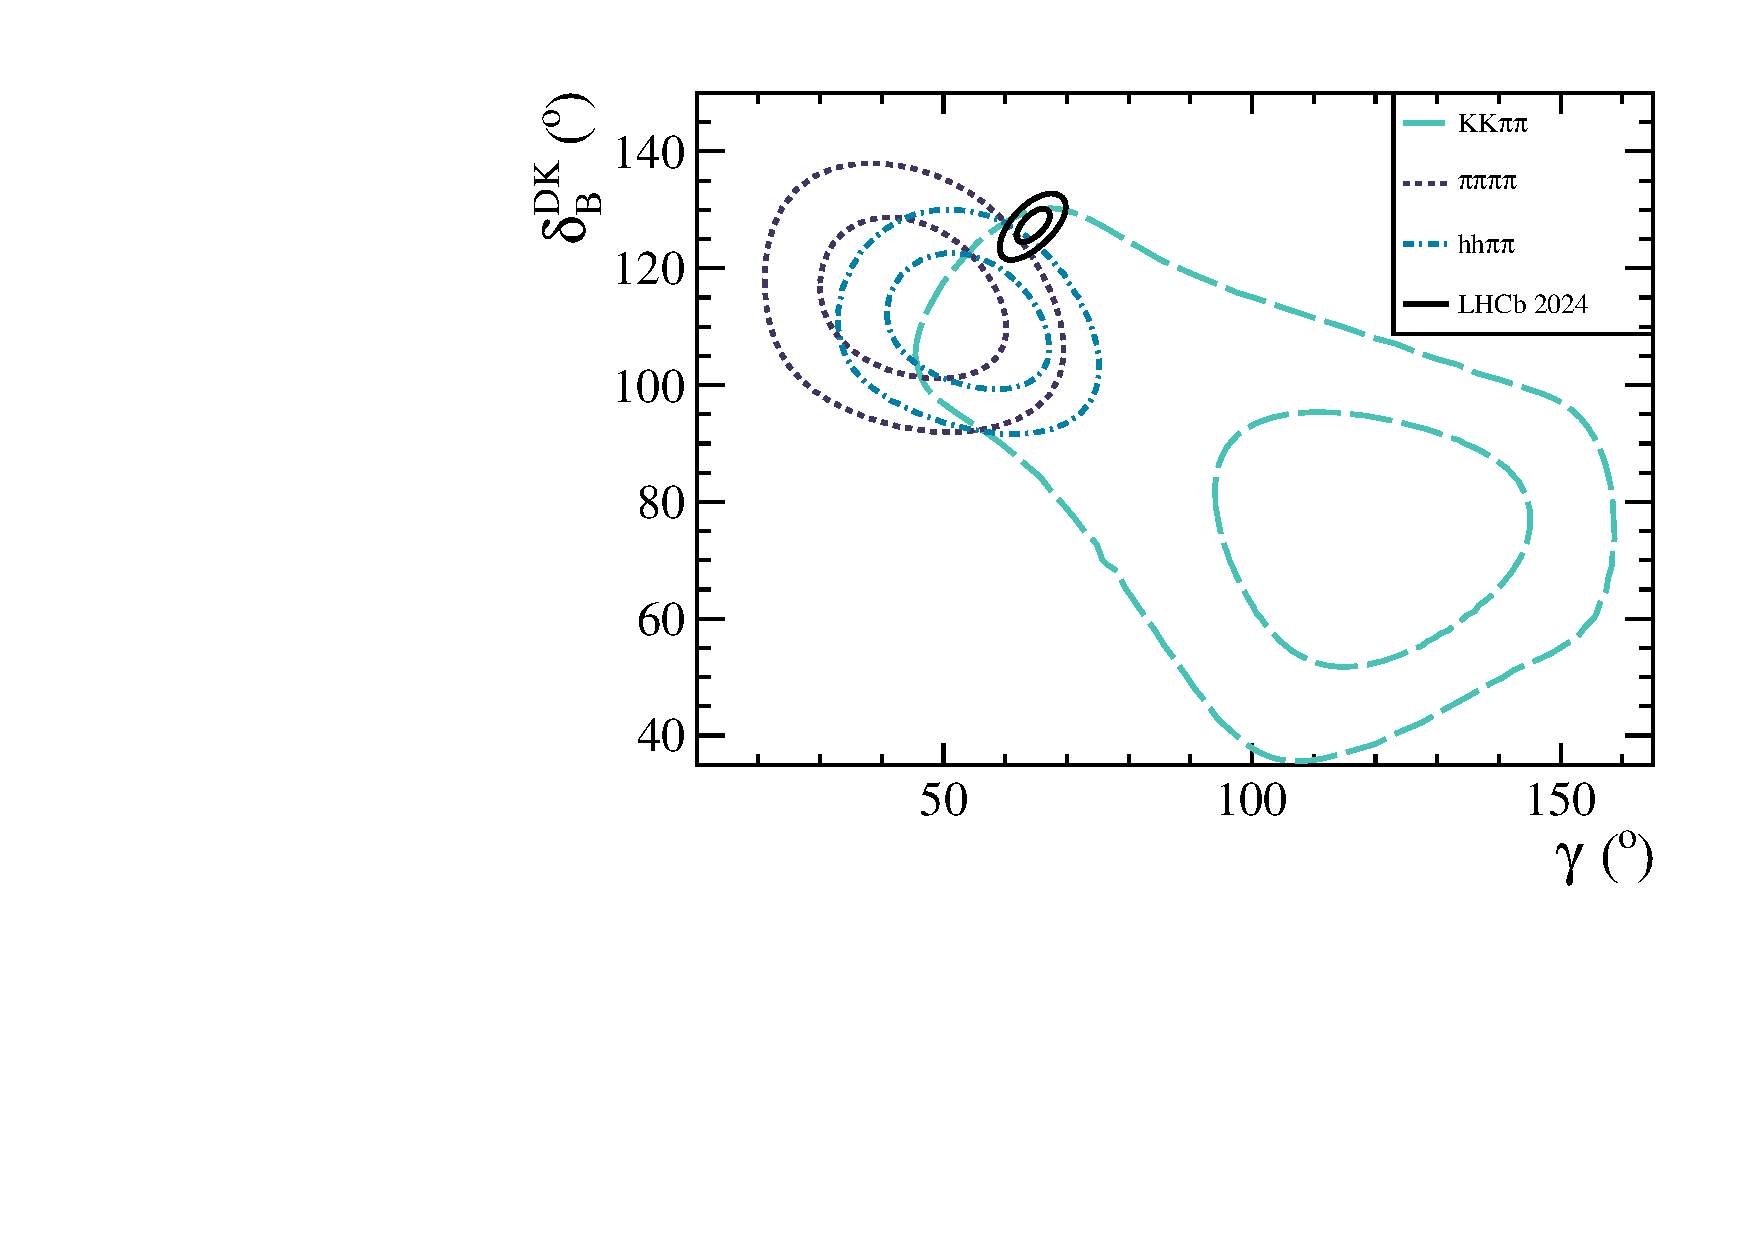
\includegraphics[width=1.0\textwidth]{Plots/gamma_deltaB_hhpipi_LHCb_Prob_scan.pdf}
      \caption*{$\gamma$ vs $\delta_B^{DK}$}
    \end{subfigure}%
    \begin{subfigure}{0.50\textwidth}
      \centering
      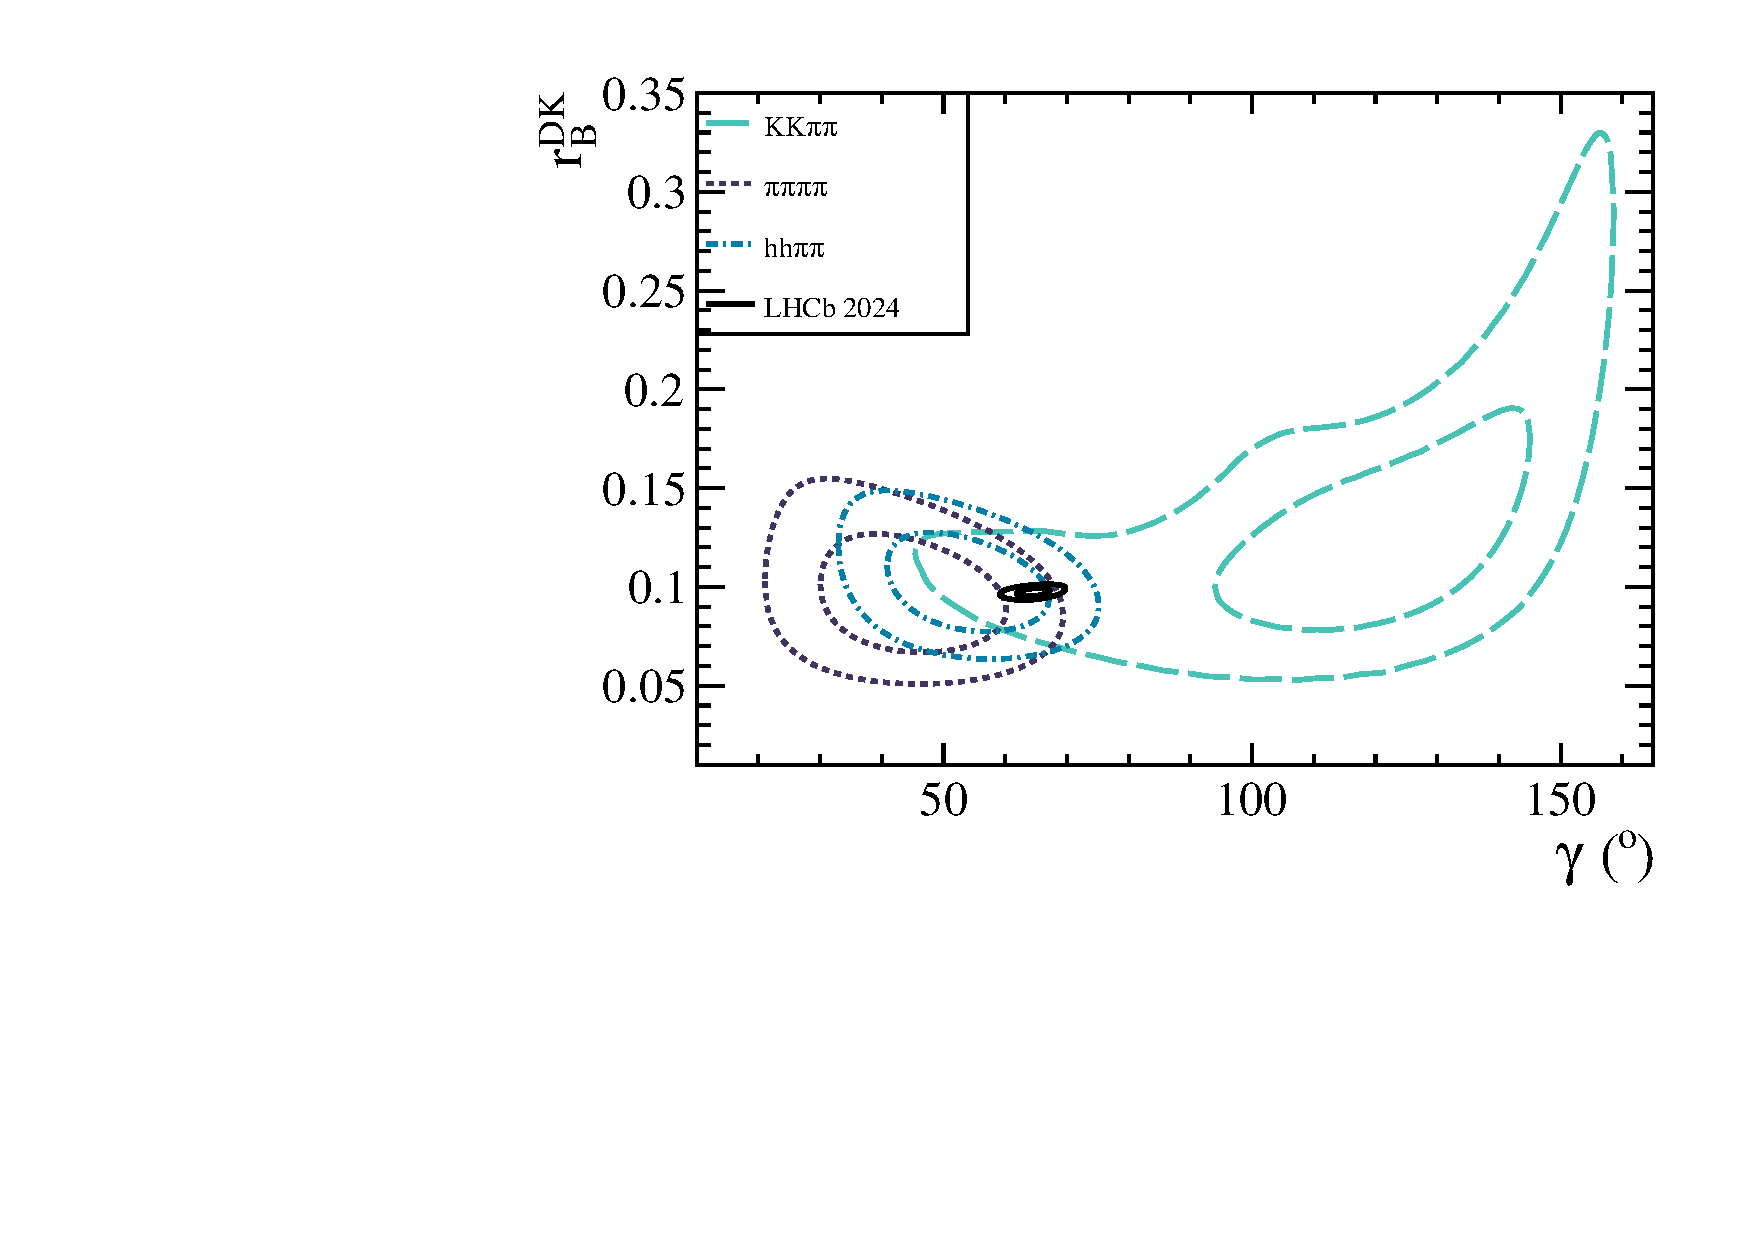
\includegraphics[width=1.0\textwidth]{Plots/gamma_rB_hhpipi_LHCb_Prob_scan.pdf}
      \caption*{$\gamma$ vs $r_B^{DK}$}
    \end{subfigure}
  \end{figure}
  \vspace{-0.3cm}
  \begin{center}
    When all biases, correlations and non-Gaussian uncertainties are accounted for, the tension with the LHCb average has reduced significantly
  \end{center}
\end{frame}

\begin{frame}{Likelihood scan of interpretation fit}
  \begin{center}
    In fact, a likelihood scan shows that $D\to K^+K^-\pi^+\pi^-$ and $D\to\pi^+\pi^-\pi^+\pi^-$ $2\sigma$ contours overlap
  \end{center}
  \begin{figure}
    \centering
    \begin{subfigure}{0.50\textwidth}
      \centering
      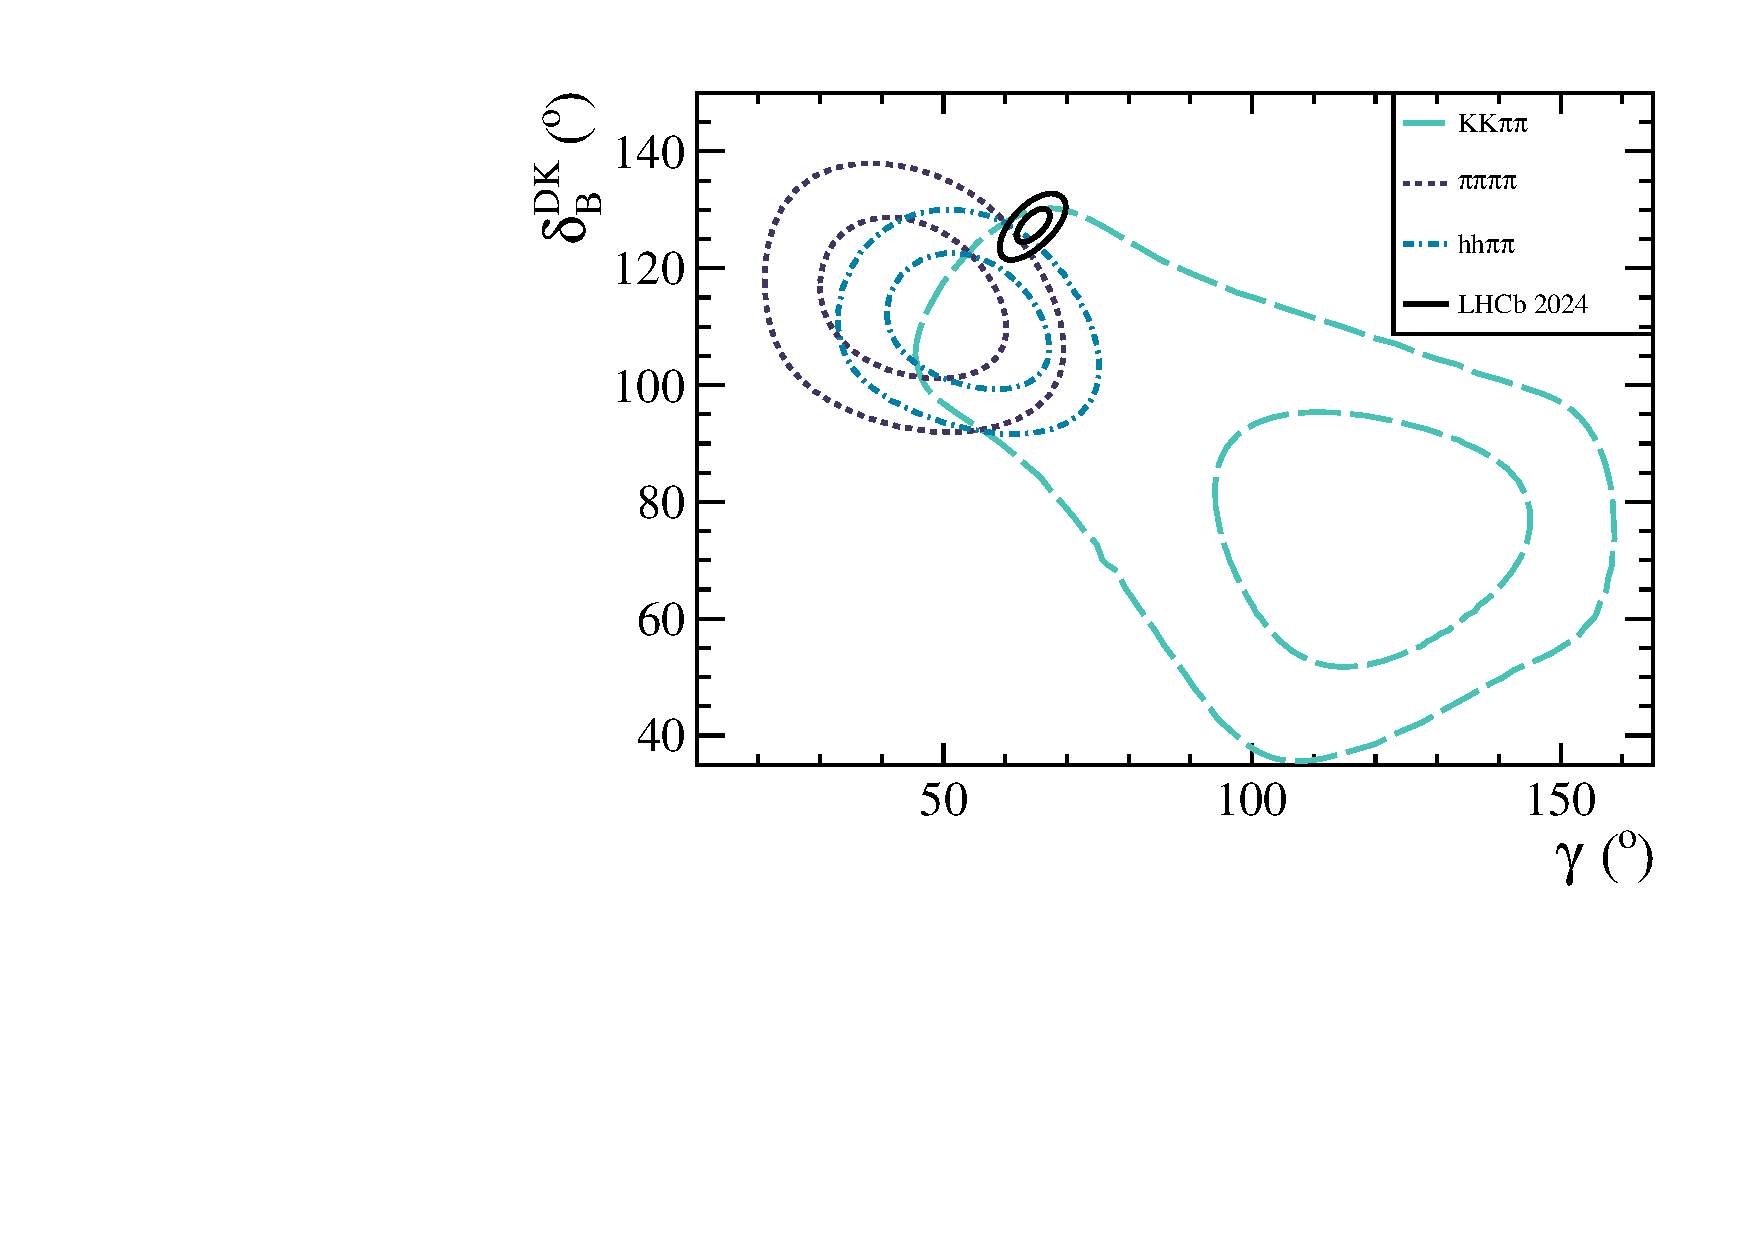
\includegraphics[width=1.0\textwidth]{Plots/gamma_deltaB_hhpipi_LHCb_Prob_scan.pdf}
      \caption*{$\gamma$ vs $\delta_B^{DK}$}
    \end{subfigure}%
    \begin{subfigure}{0.50\textwidth}
      \centering
      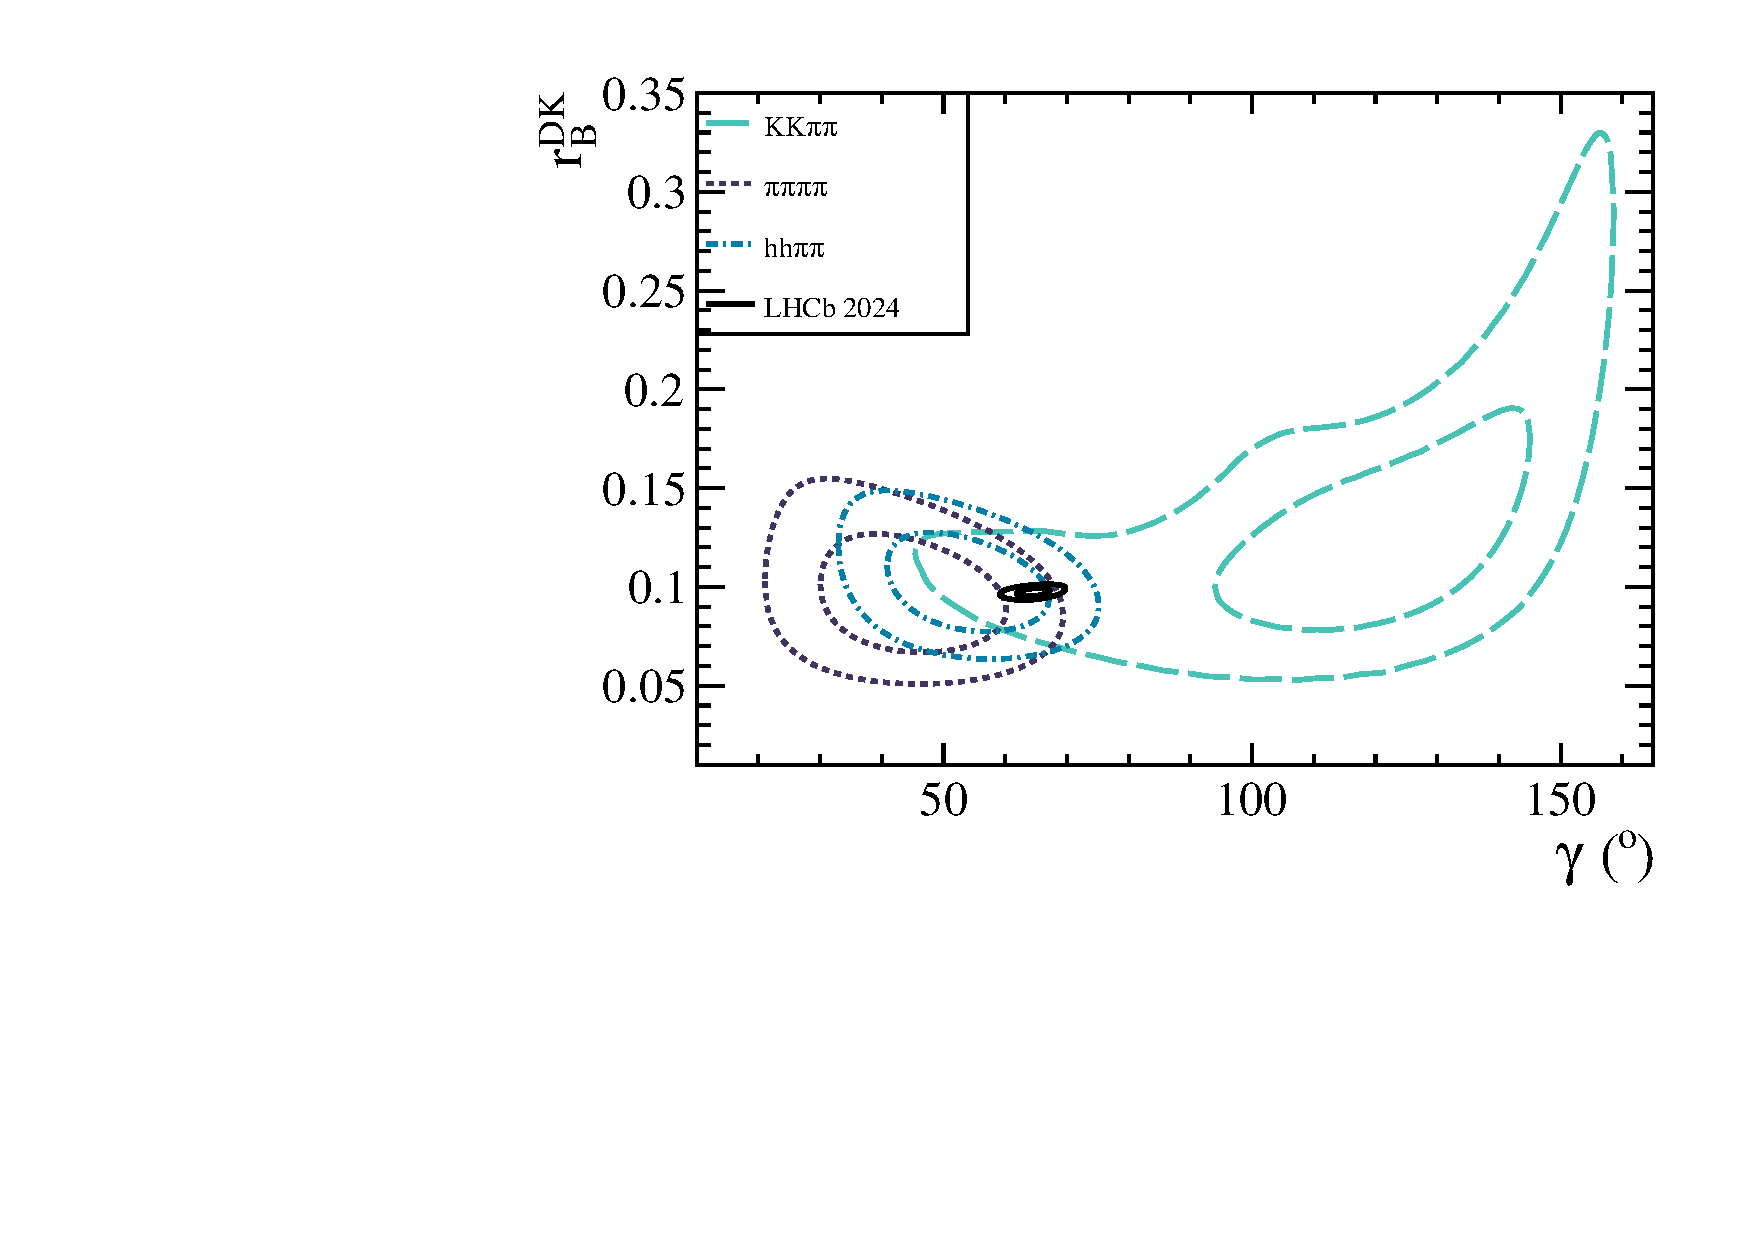
\includegraphics[width=1.0\textwidth]{Plots/gamma_rB_hhpipi_LHCb_Prob_scan.pdf}
      \caption*{$\gamma$ vs $r_B^{DK}$}
    \end{subfigure}
  \end{figure}
  \vspace{-0.3cm}
  \begin{center}
    However, with all the non-Gaussian behaviour, are we sure these contours cover $68\%$ and $95\%$\phantom{y}?
  \end{center}
\end{frame}

\begin{frame}{Plugin/Feldman-Cousins method}
  \begin{center}
    {\Large Feldman-Cousins method, or Plugin, is a ``brute-force'' approach to assigning a confidence interval} \\~\\
    {At each scan point of $\gamma$, perform these fits to data:}
  \end{center}
  \begin{enumerate}
    \setlength\itemsep{0.5em}
    \item{Fit with all parameters floating, and save the log-likelihood $\chi^2$}
    \item{Fit with $\gamma$ fixed to scan point, and save $\chi^2_{\rm fix}$}
    \item{Calculate $\Delta\chi^2_{\rm data} = \chi^2_{\rm fix} - \chi^2$}
  \end{enumerate}
  \vspace{0.5cm}
  \begin{center}
    {We expect $\Delta\chi^2_{\rm data}$ to become large as we move away from best-fit value, but without direct knowledge of underlying PDF, we cannot determine any confidence intervals from this}
  \end{center}
\end{frame}

\begin{frame}{Plugin/Feldman-Cousins method}
  \begin{center}
    {\Large Feldman-Cousins method, or Plugin, is a ``brute-force'' approach to assigning a confidence interval} \\~\\
    {At each scan point of $\gamma$, perform these fits to toy:}
  \end{center}
  \begin{enumerate}
    \setlength\itemsep{0.5em}
    \item{Fix $\gamma$ to scan point and generate $1000$ toys}
    \item{Perform fits to each toy, with $\gamma$ both floating and fixed}
    \item{Calculate $\Delta\chi^2_{\rm toy}$}
  \end{enumerate}
  \vspace{0.42cm}
  \begin{center}
    {At each scan point, the fraction of toys with $\Delta\chi^2_{\rm toy} > \Delta\chi^2_{\rm data}$ is equal to $1 - \rm{CL}$, and the exact $68\%$ confidence interval can then be obtained using an interpolation between points}
  \end{center}
\end{frame}

\begin{frame}{Plugin/Feldman-Cousins method}
  \begin{center}
    LHCb average within $2\sigma$ of $D\to K^+K^-\pi^+\pi^-$ Plugin result \\
    Combined fit shows good agreement between Plugin and Prob scans
  \end{center}
  \begin{figure}
    \centering
    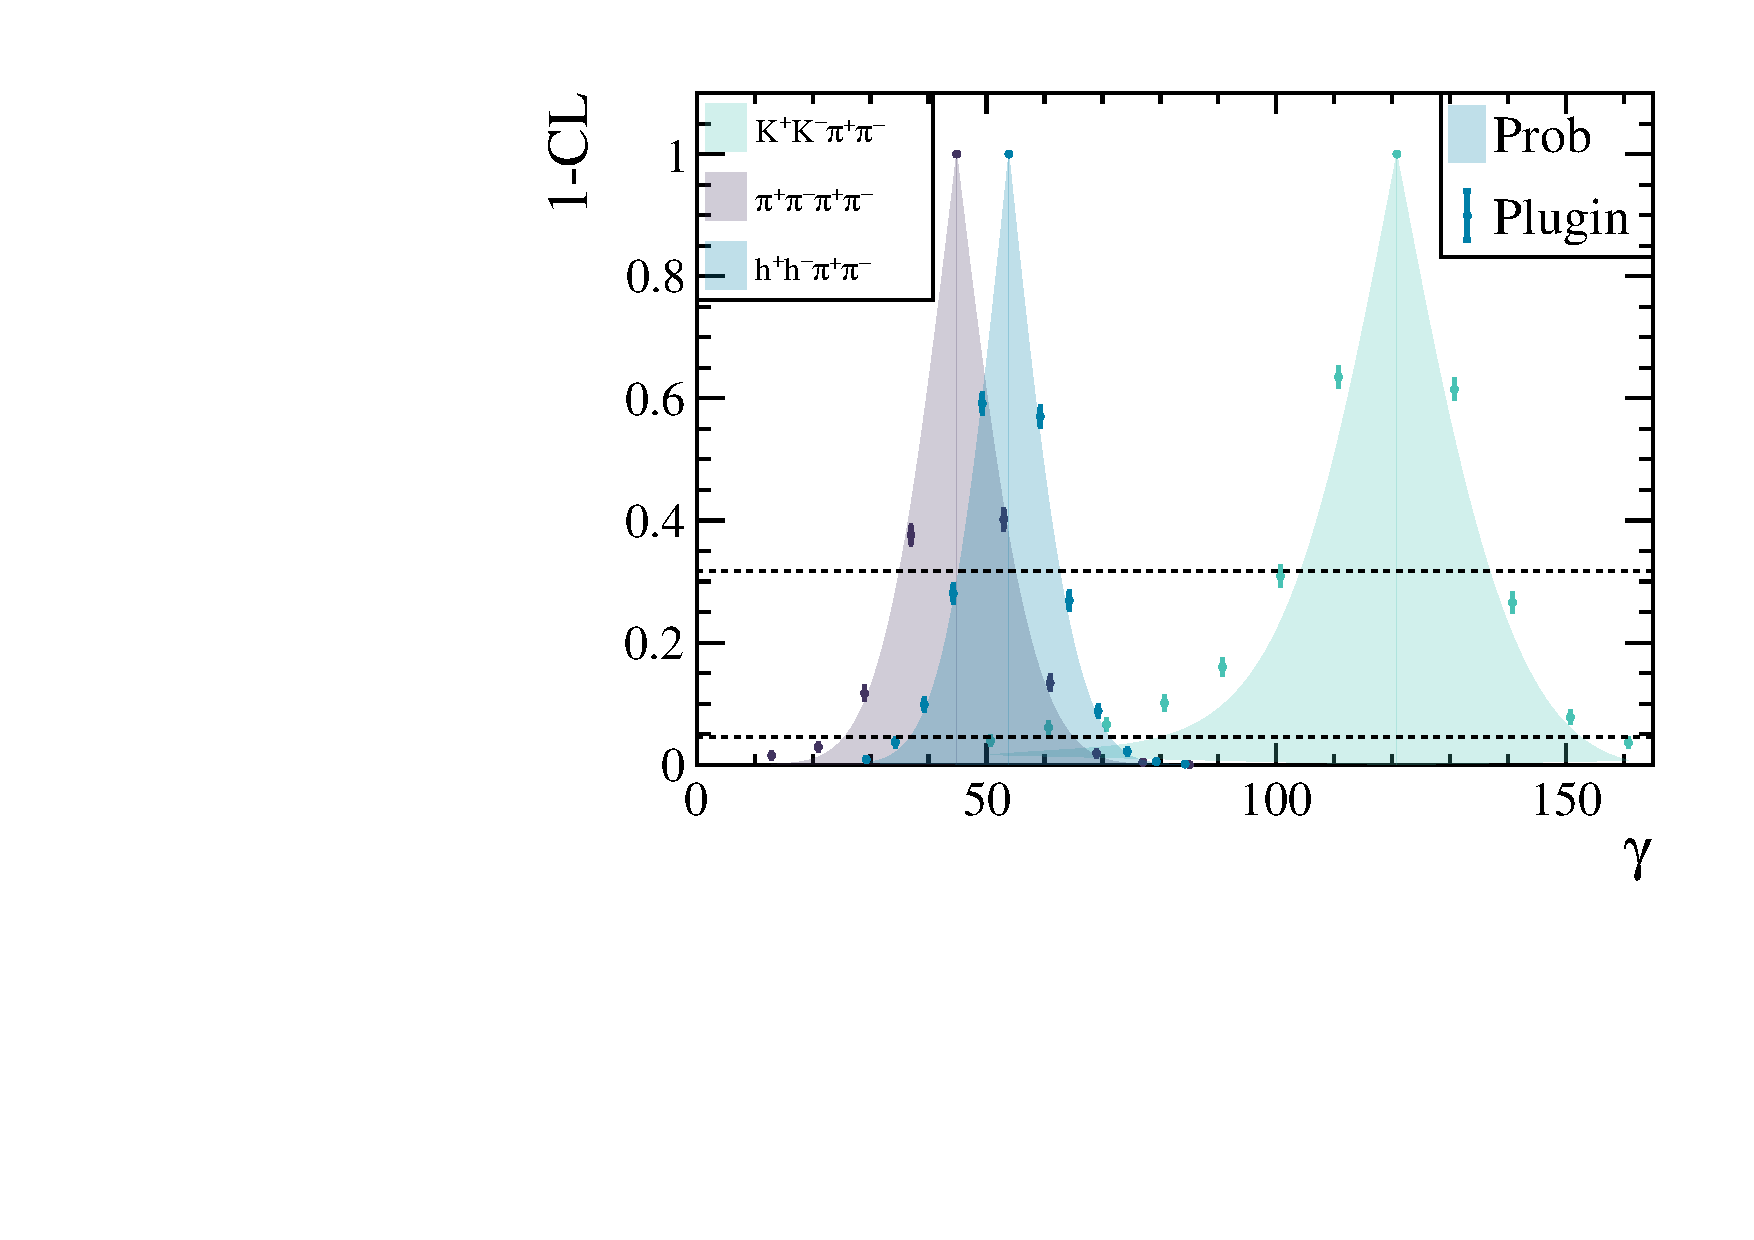
\includegraphics[width=0.6\textwidth]{Plots/gamma_plugin_scan.pdf}
  \end{figure}
  \vspace{-0.3cm}
  \begin{center}
    Combined fit result: $\gamma = (53.9_{-8.9}^{+9.5})^\circ$ \\
    One of the most precise single measurements of $\gamma$!
  \end{center}
\end{frame}

\begin{frame}{Combining phase-space binned and integrated results}
  \begin{center}
    We can add phase-space integrated observables as a constraint:
  \end{center}
  \begin{figure}
    \centering
    \begin{subfigure}{0.50\textwidth}
      \centering
      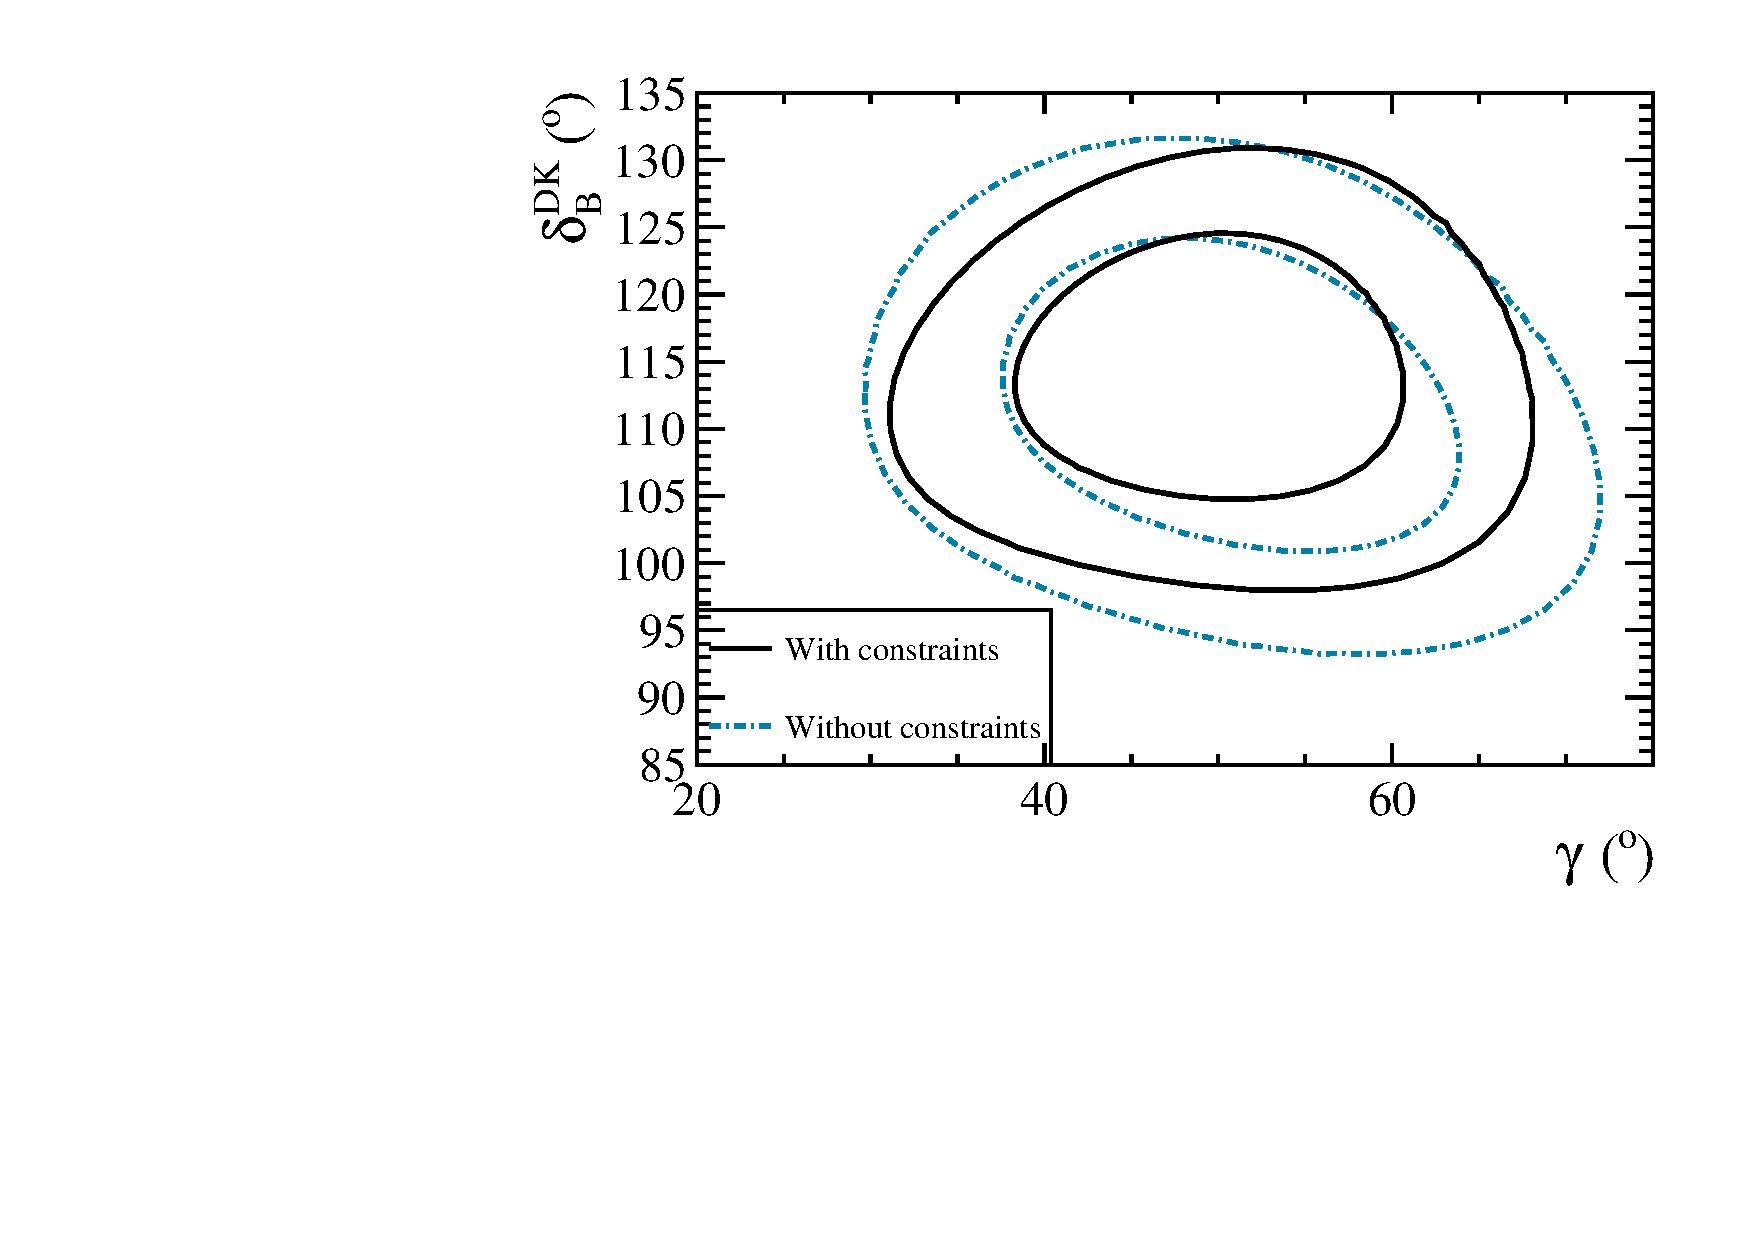
\includegraphics[width=1.0\textwidth]{Plots/GLW_constraints_comparison_gamma_deltaB.pdf}
      \caption*{$\gamma$ vs $\delta_B^{DK}$}
    \end{subfigure}%
    \begin{subfigure}{0.50\textwidth}
      \centering
      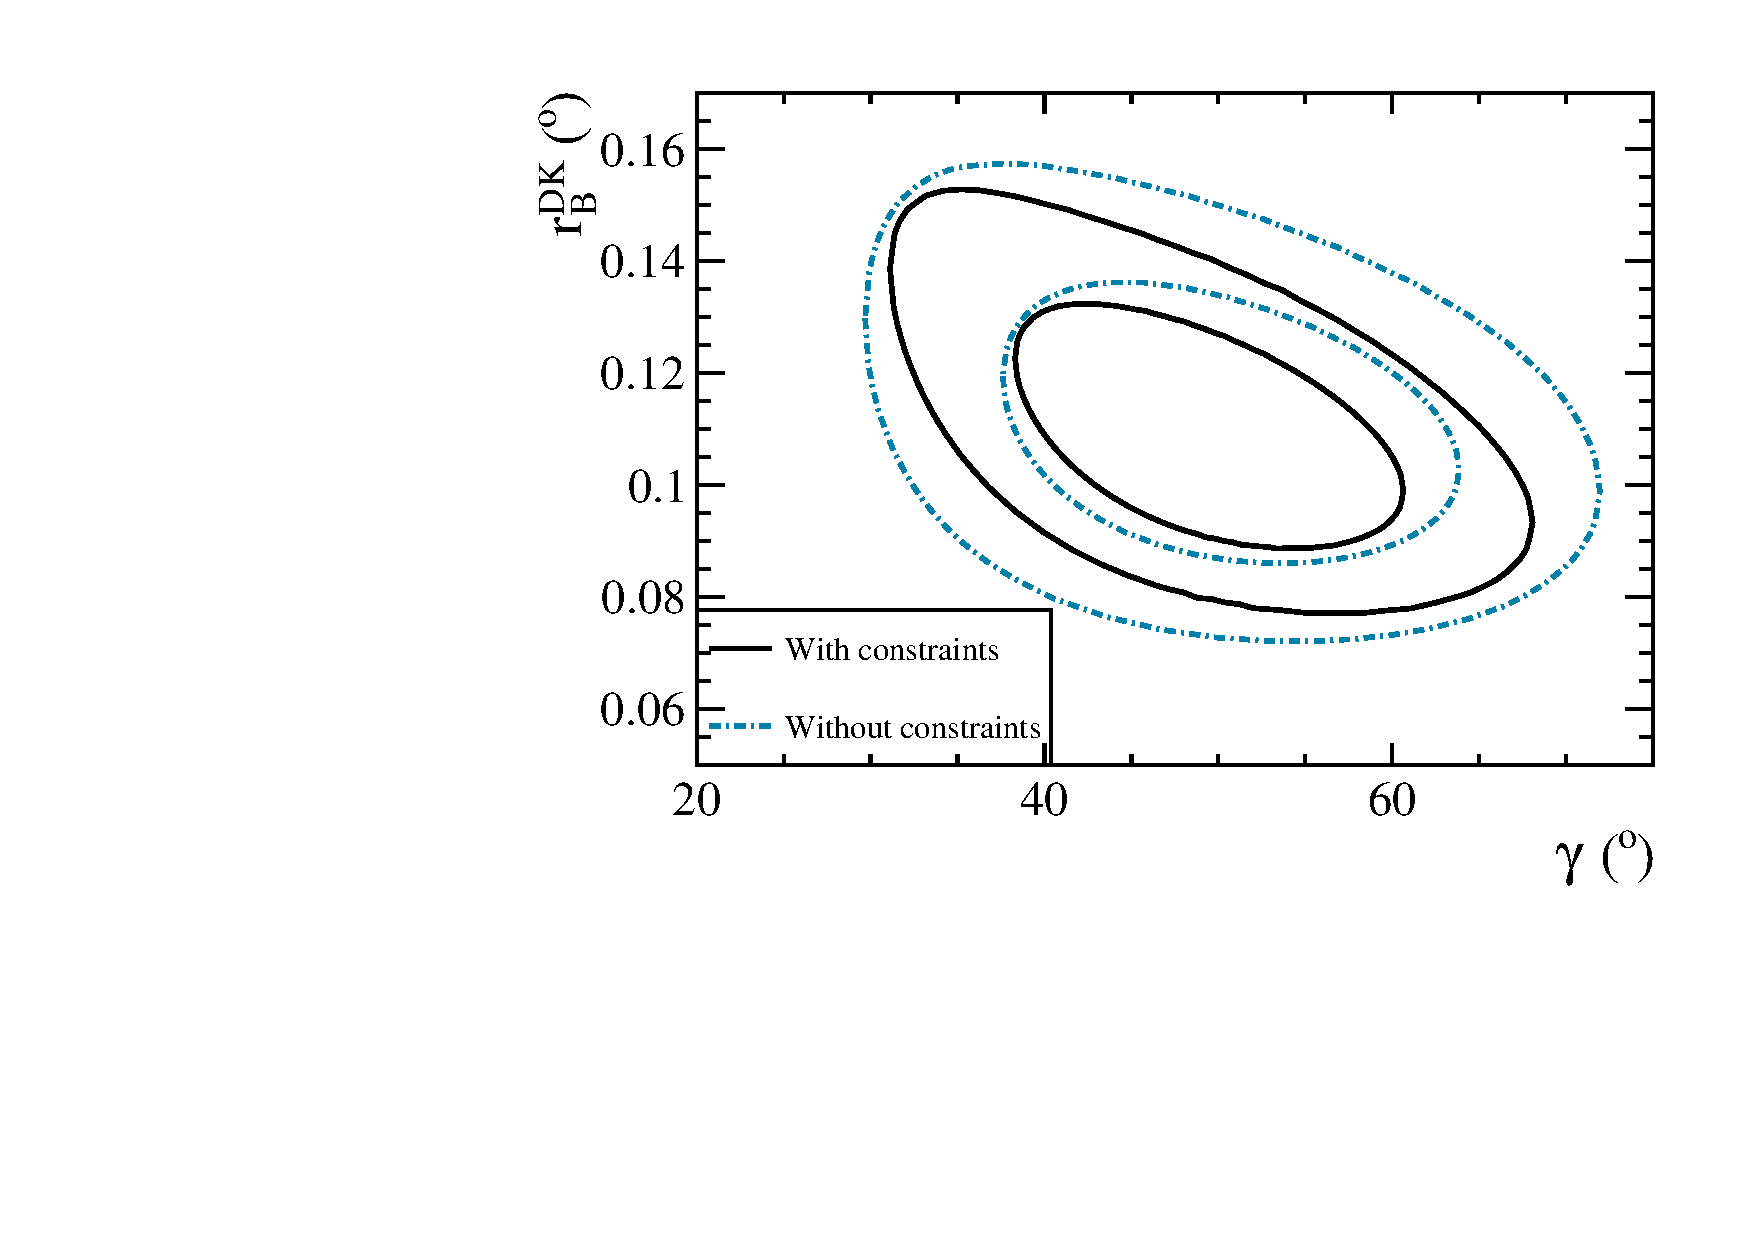
\includegraphics[width=1.0\textwidth]{Plots/GLW_constraints_comparison_gamma_rB.pdf}
      \caption*{$\gamma$ vs $r_B^{DK}$}
    \end{subfigure}
  \end{figure}
  \vspace{-0.3cm}
  \begin{center}
    The global asymmetries contain useful information!
  \end{center}
\end{frame}

\begin{frame}{Combining phase-space binned and integrated results}
  \begin{center}
    Run Plugin with phase-space integrated constraints:
  \end{center}
  \begin{figure}
    \centering
    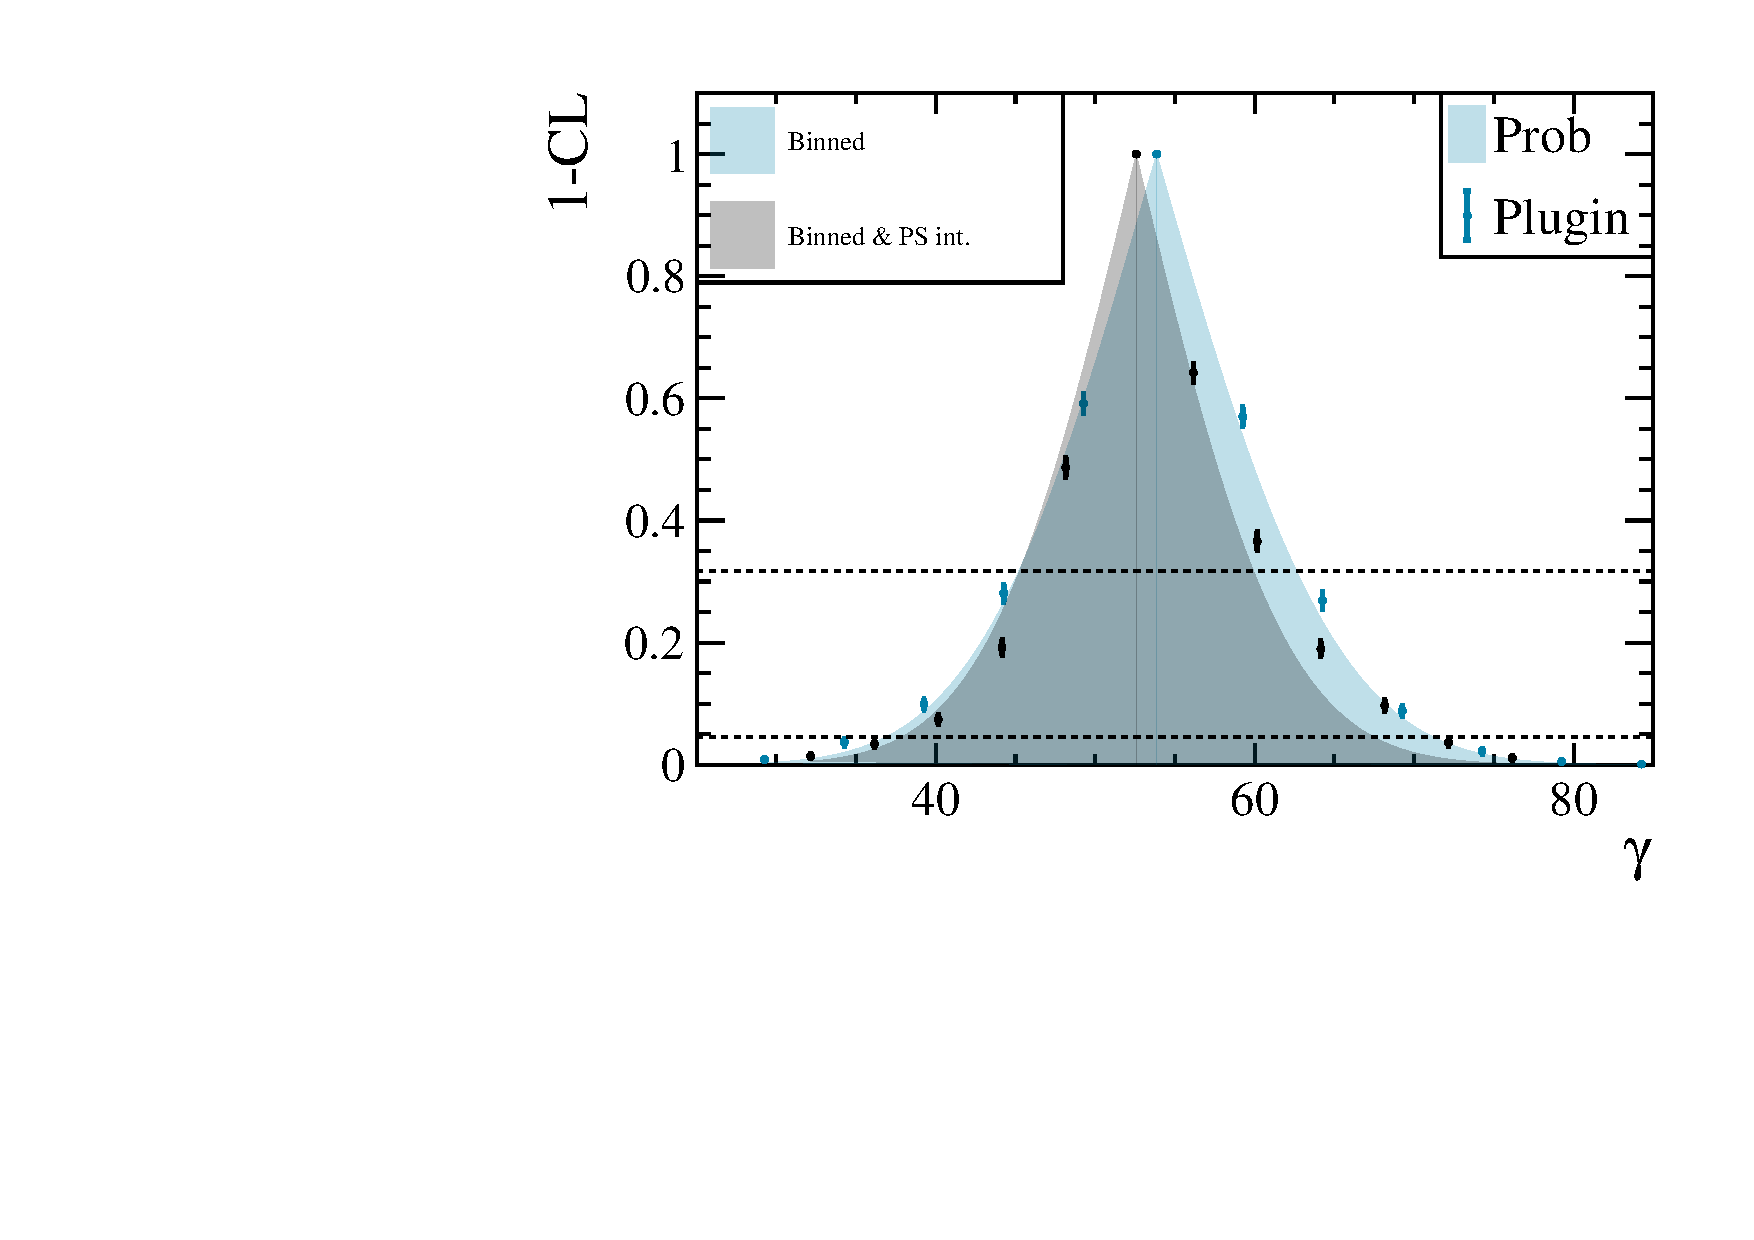
\includegraphics[width=0.6\textwidth]{Plots/gamma_plugin_scan_GLW.pdf}
  \end{figure}
  \vspace{-0.3cm}
  \begin{center}
    Final measurement: $\gamma = (52.6_{-6.4}^{+8.5})^\circ$ \\
  \end{center}
\end{frame}

\section{Conclusion and future prospects}
\begin{frame}{Conclusion}
  \vspace{-0.1cm}
  \begin{enumerate}
    \setlength\itemsep{1.5em}
    \item{Binned model-independent measurement of $\gamma$ with $B^\pm\to[h^+h^-\pi^+\pi^-]_Dh^\pm$ has been performed}
    \begin{itemize}
      \item{Result: $\gamma = (53.9_{-8.9}^{+9.5})^\circ$}
    \end{itemize}
    \item{Can also combine with existing phase-space integrated measurements}
    \begin{itemize}
      \item{Result: $\gamma = (52.6_{-6.4}^{+8.5})^\circ$}
    \end{itemize}
    \item{$3\sigma$ tension in $D\to K^+K^-\pi^+\pi^-$ has reduced}
  \end{enumerate}
\end{frame}

\begin{frame}{Future prospects}
  \vspace{0.6cm}
  \begin{itemize}
    \setlength\itemsep{1.4em}
    \item{Statistically limited measurement, but $s_i$ uncertainties are large}
    \item{$\pi^+\pi^-\pi^+\pi^-$ inputs will become more precise:}
    \begin{itemize}
      \item{Current analysis uses $\SI{3}{\per\femto\barn}$}
      \item{Future updates will use the full $\SI{20}{\per\femto\barn}$ data set}
    \end{itemize}
    \item{Minor improvements from BESIII are expected with $K^+K^-\pi^+\pi^-$:}
    \begin{itemize}
      \item{Current analysis already uses $\SI{20}{\per\femto\barn}$}
      \item{Charm mixing studies can improve $s_i$ precision}
    \end{itemize}
    \item{We believe the analysis is ready for approval to go to paper}
    \begin{itemize}
      \item{You can find the TWiki \href{https://twiki.cern.ch/twiki/bin/viewauth/LHCbPhysics/BPGGSZB2DhD2hhpipiModelIndependent}{here}}
    \end{itemize}
  \end{itemize}
  \vspace{0.3cm}
  \begin{center}
    {\huge Thanks for your attention!}
  \end{center}
\end{frame}

\begin{frame}{Backup: CP fit toy studies}
  \begin{center}
    In toy studies biases in $D\pi$ observables are consistent with model-dependent analysis
  \end{center}
  \begin{figure}
    \centering
    \begin{subfigure}{0.5\textwidth}
      \centering
      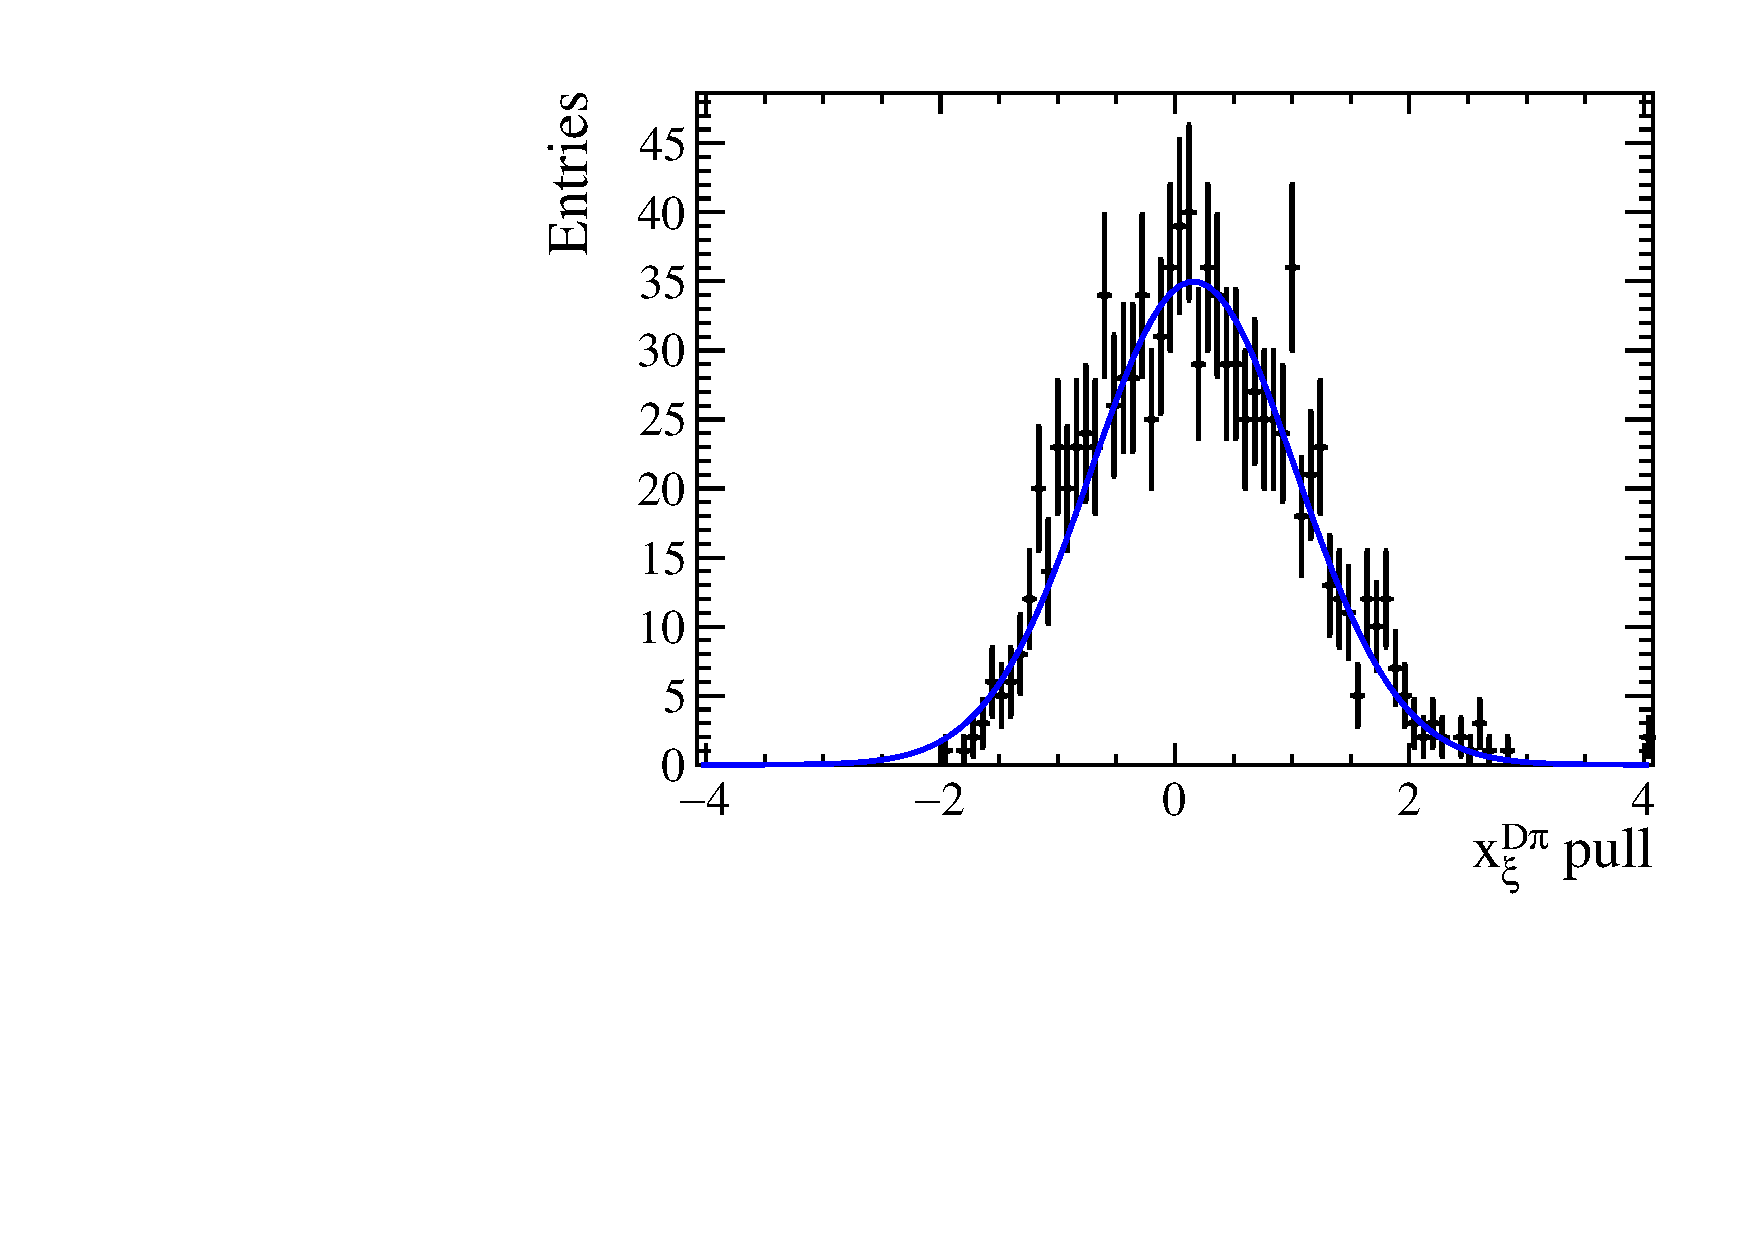
\includegraphics[width=1.0\textwidth]{Plots/A_Re_xi_dpi_pull.pdf}
      \vspace{-0.3cm}
      \caption*{$x_\xi^{D\pi}$}
    \end{subfigure}%
    \begin{subfigure}{0.5\textwidth}
      \centering
      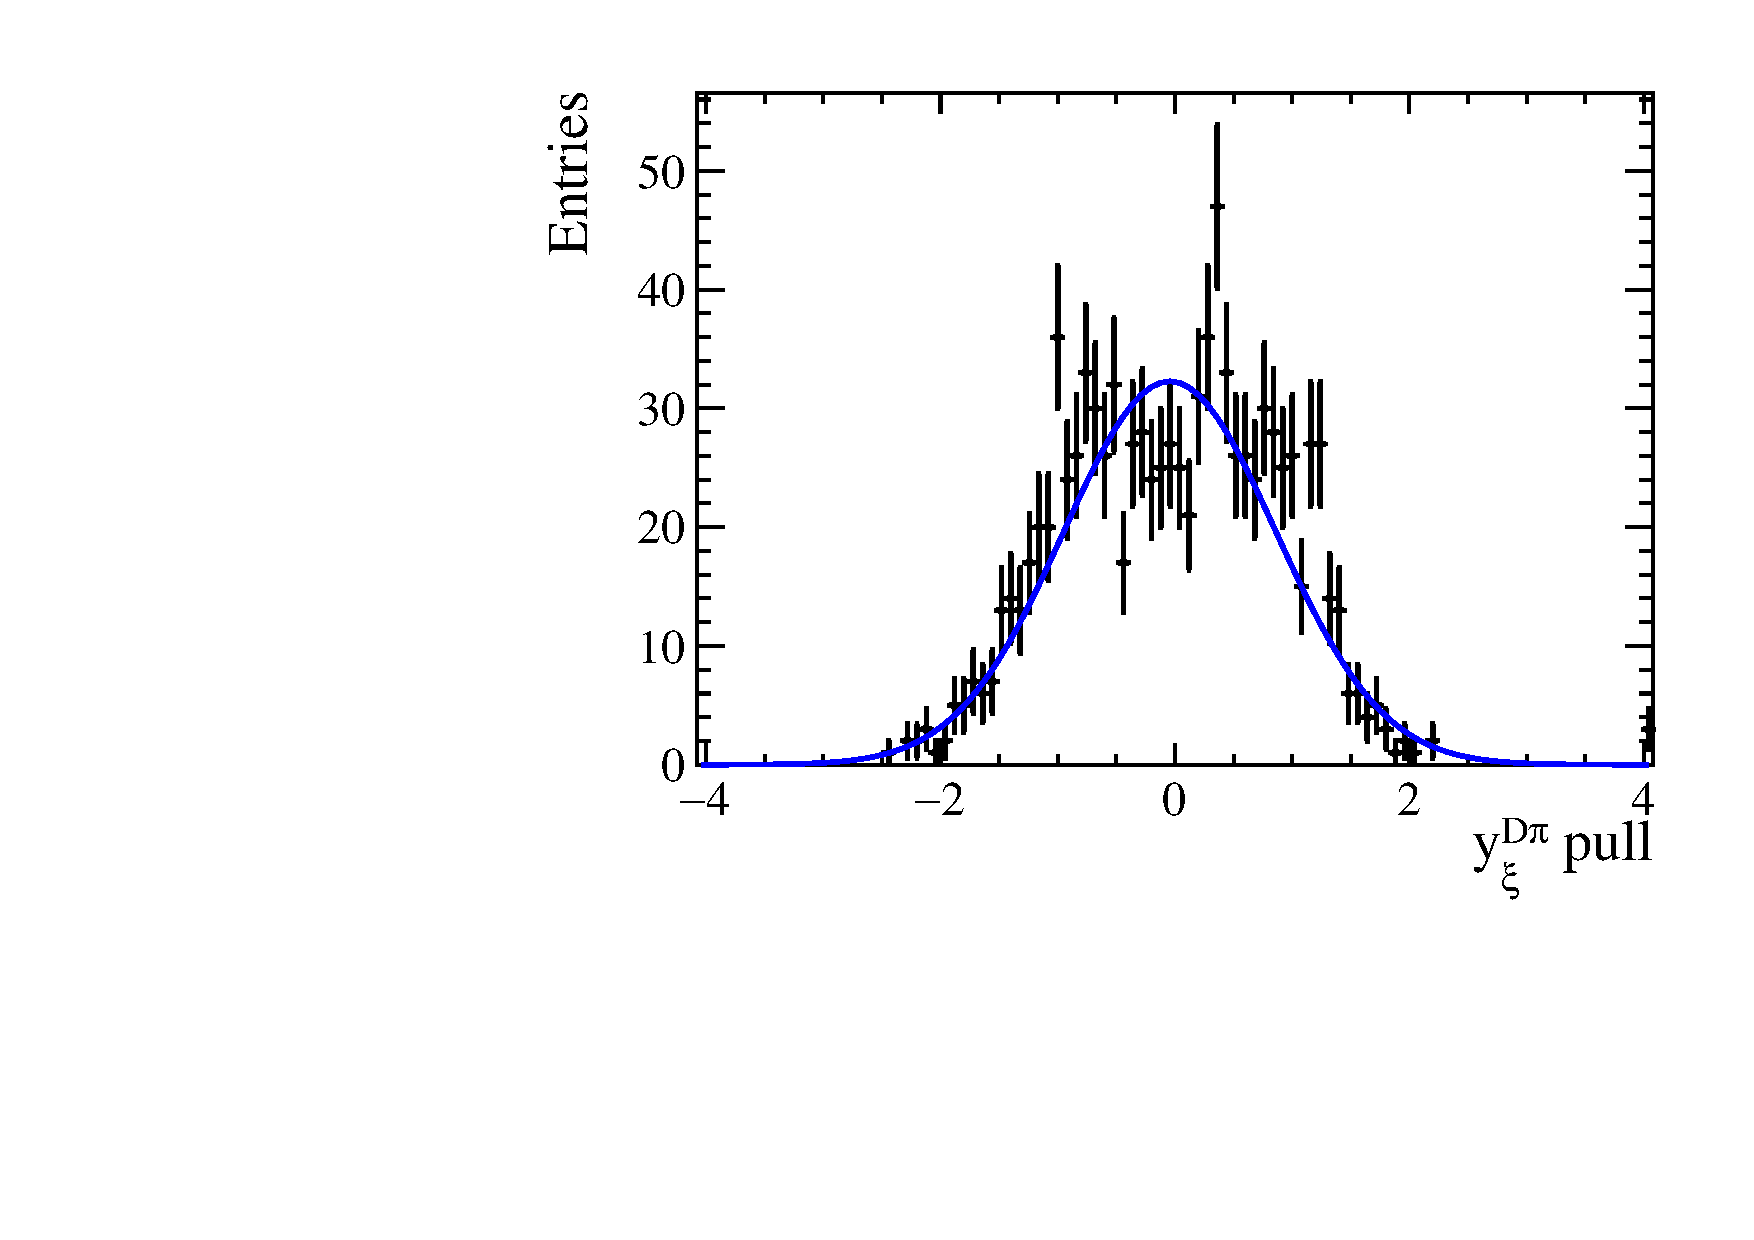
\includegraphics[width=1.0\textwidth]{Plots/A_Im_xi_dpi_pull.pdf}
      \vspace{-0.3cm}
      \caption*{$y_\xi^{D\pi}$}
    \end{subfigure}
    \caption*{$D^0\to K^+K^-\pi^+\pi^-$}
  \end{figure}
\end{frame}

\begin{frame}{Backup: CP fit toy studies}
  \begin{center}
    Minor biases in $x_\pm^{DK}$ are seen but can be corrected for...
  \end{center}
  \begin{figure}
    \centering
    \begin{subfigure}{0.5\textwidth}
      \centering
      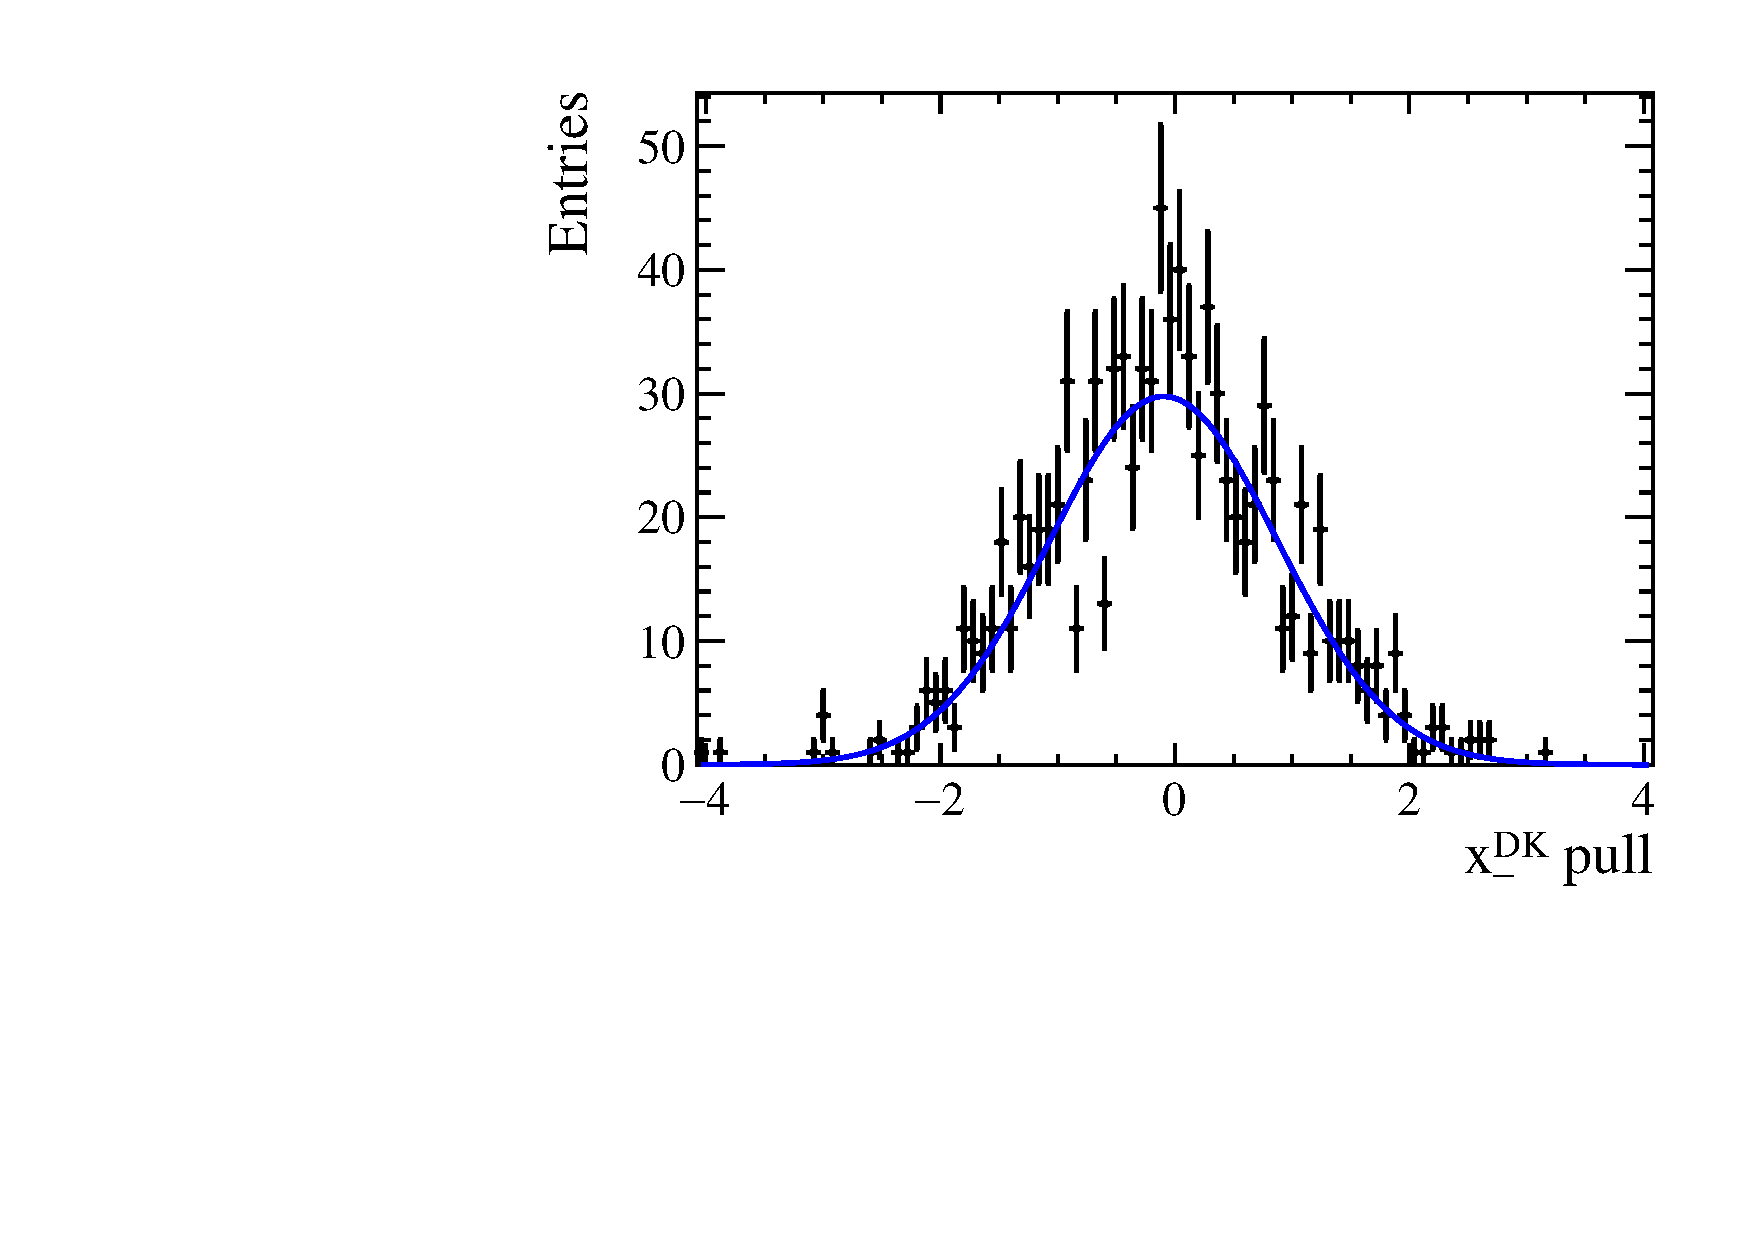
\includegraphics[width=1.0\textwidth]{Plots/A_xm_dk_pull.pdf}
      \vspace{-0.3cm}
      \caption*{$x_-^{DK}$}
    \end{subfigure}%
    \begin{subfigure}{0.5\textwidth}
      \centering
      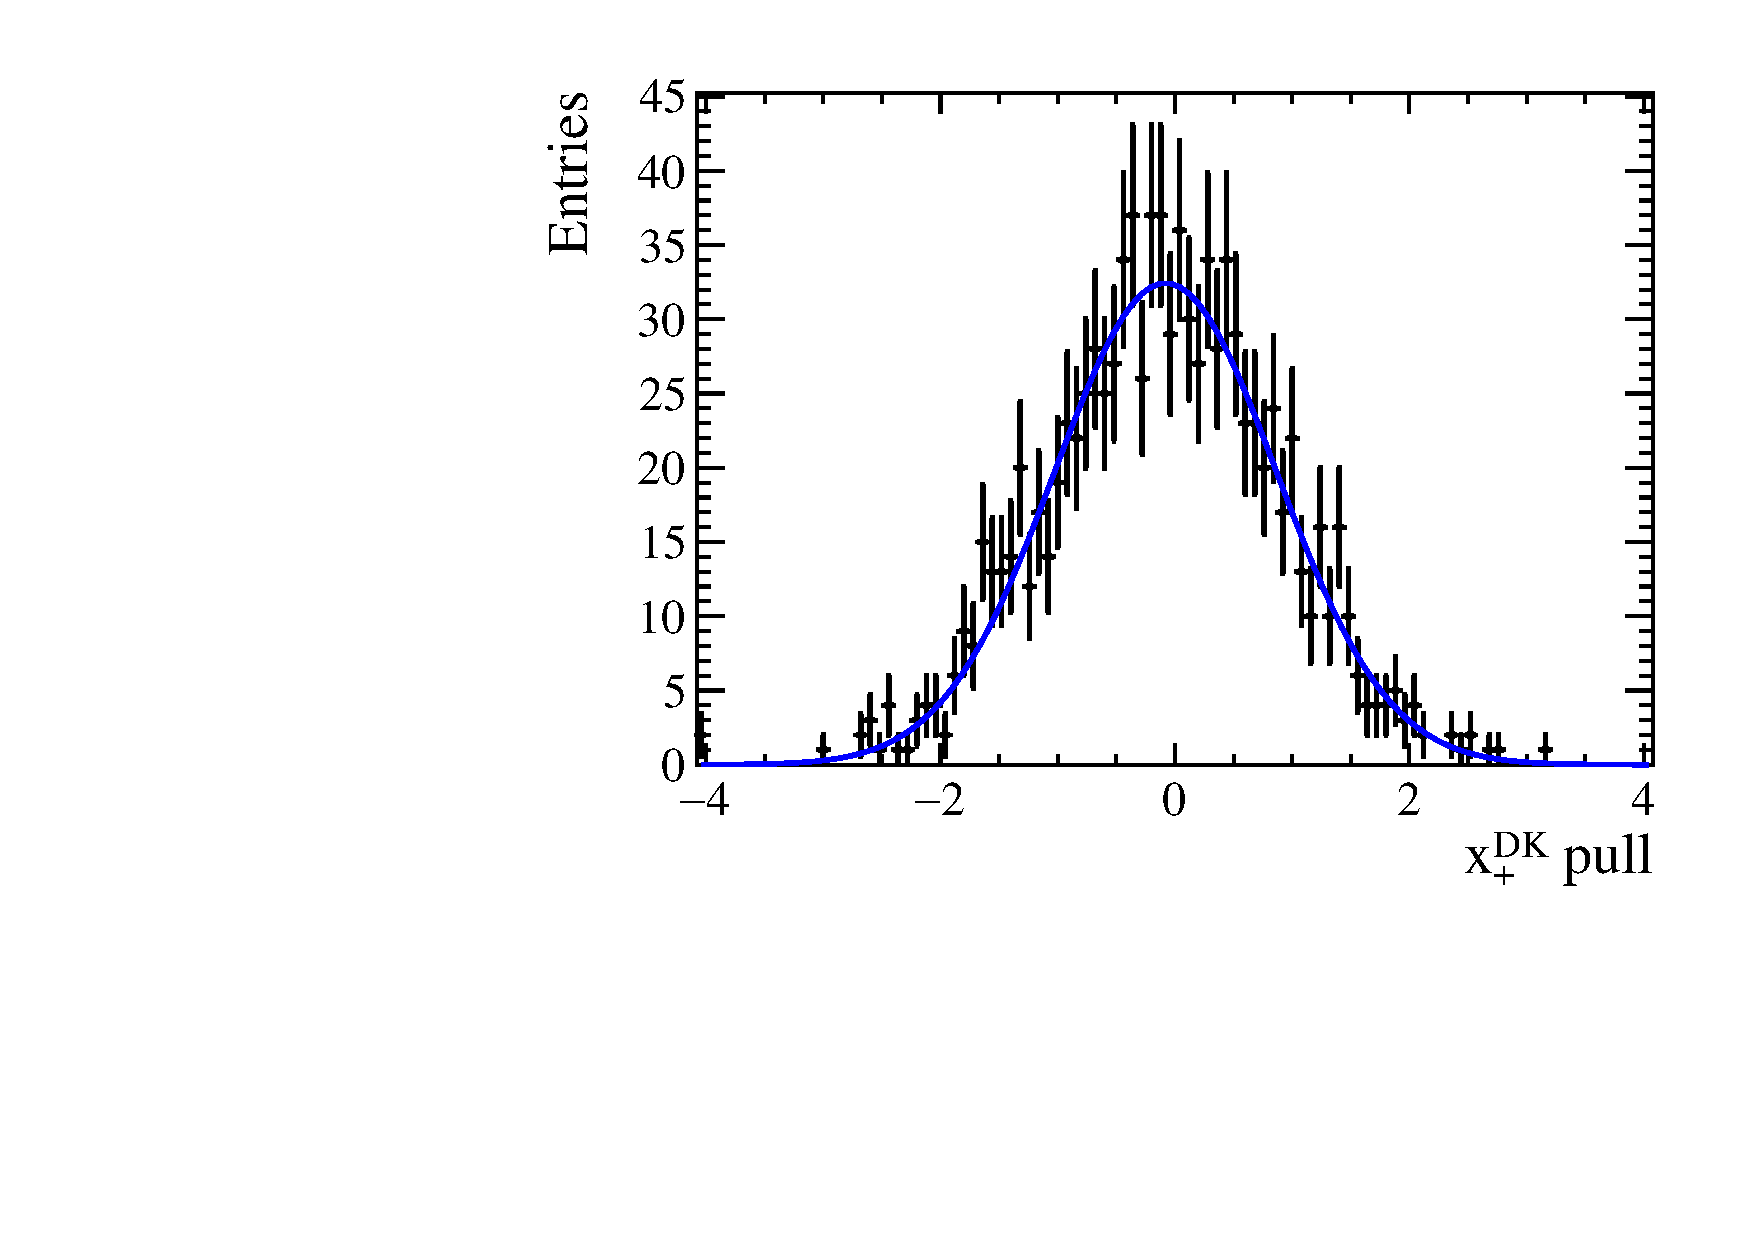
\includegraphics[width=1.0\textwidth]{Plots/A_xp_dk_pull.pdf}
      \vspace{-0.3cm}
      \caption*{$x_+^{DK}$}
    \end{subfigure}
    \caption*{$D^0\to K^+K^-\pi^+\pi^-$}
  \end{figure}
\end{frame}

\begin{frame}{Backup: CP fit toy studies}
  \begin{center}
    ...but $y_\pm^{DK}$ pulls are now slightly asymmetric!
  \end{center}
  \begin{figure}
    \centering
    \begin{subfigure}{0.5\textwidth}
      \centering
      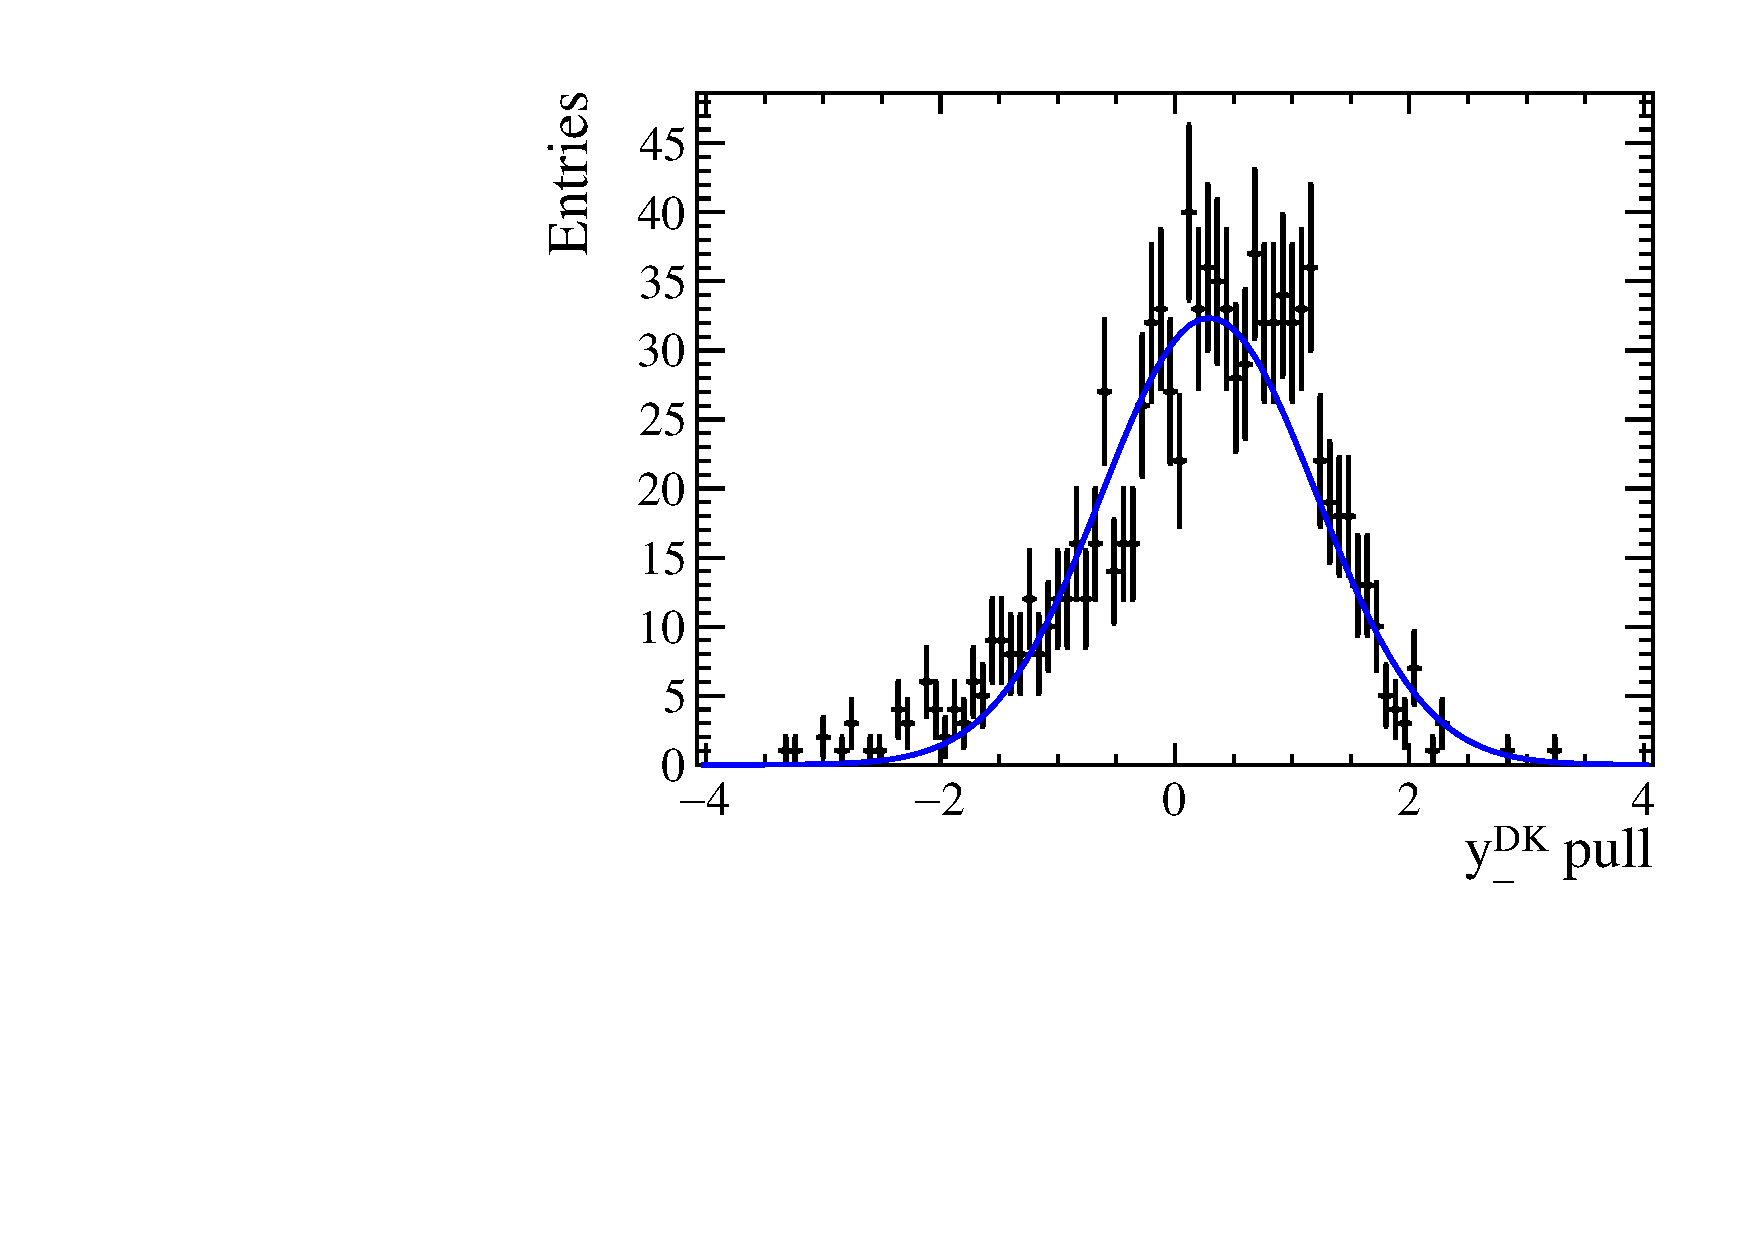
\includegraphics[width=1.0\textwidth]{Plots/A_ym_dk_pull.pdf}
      \vspace{-0.3cm}
      \caption*{$y_-^{DK}$}
    \end{subfigure}%
    \begin{subfigure}{0.5\textwidth}
      \centering
      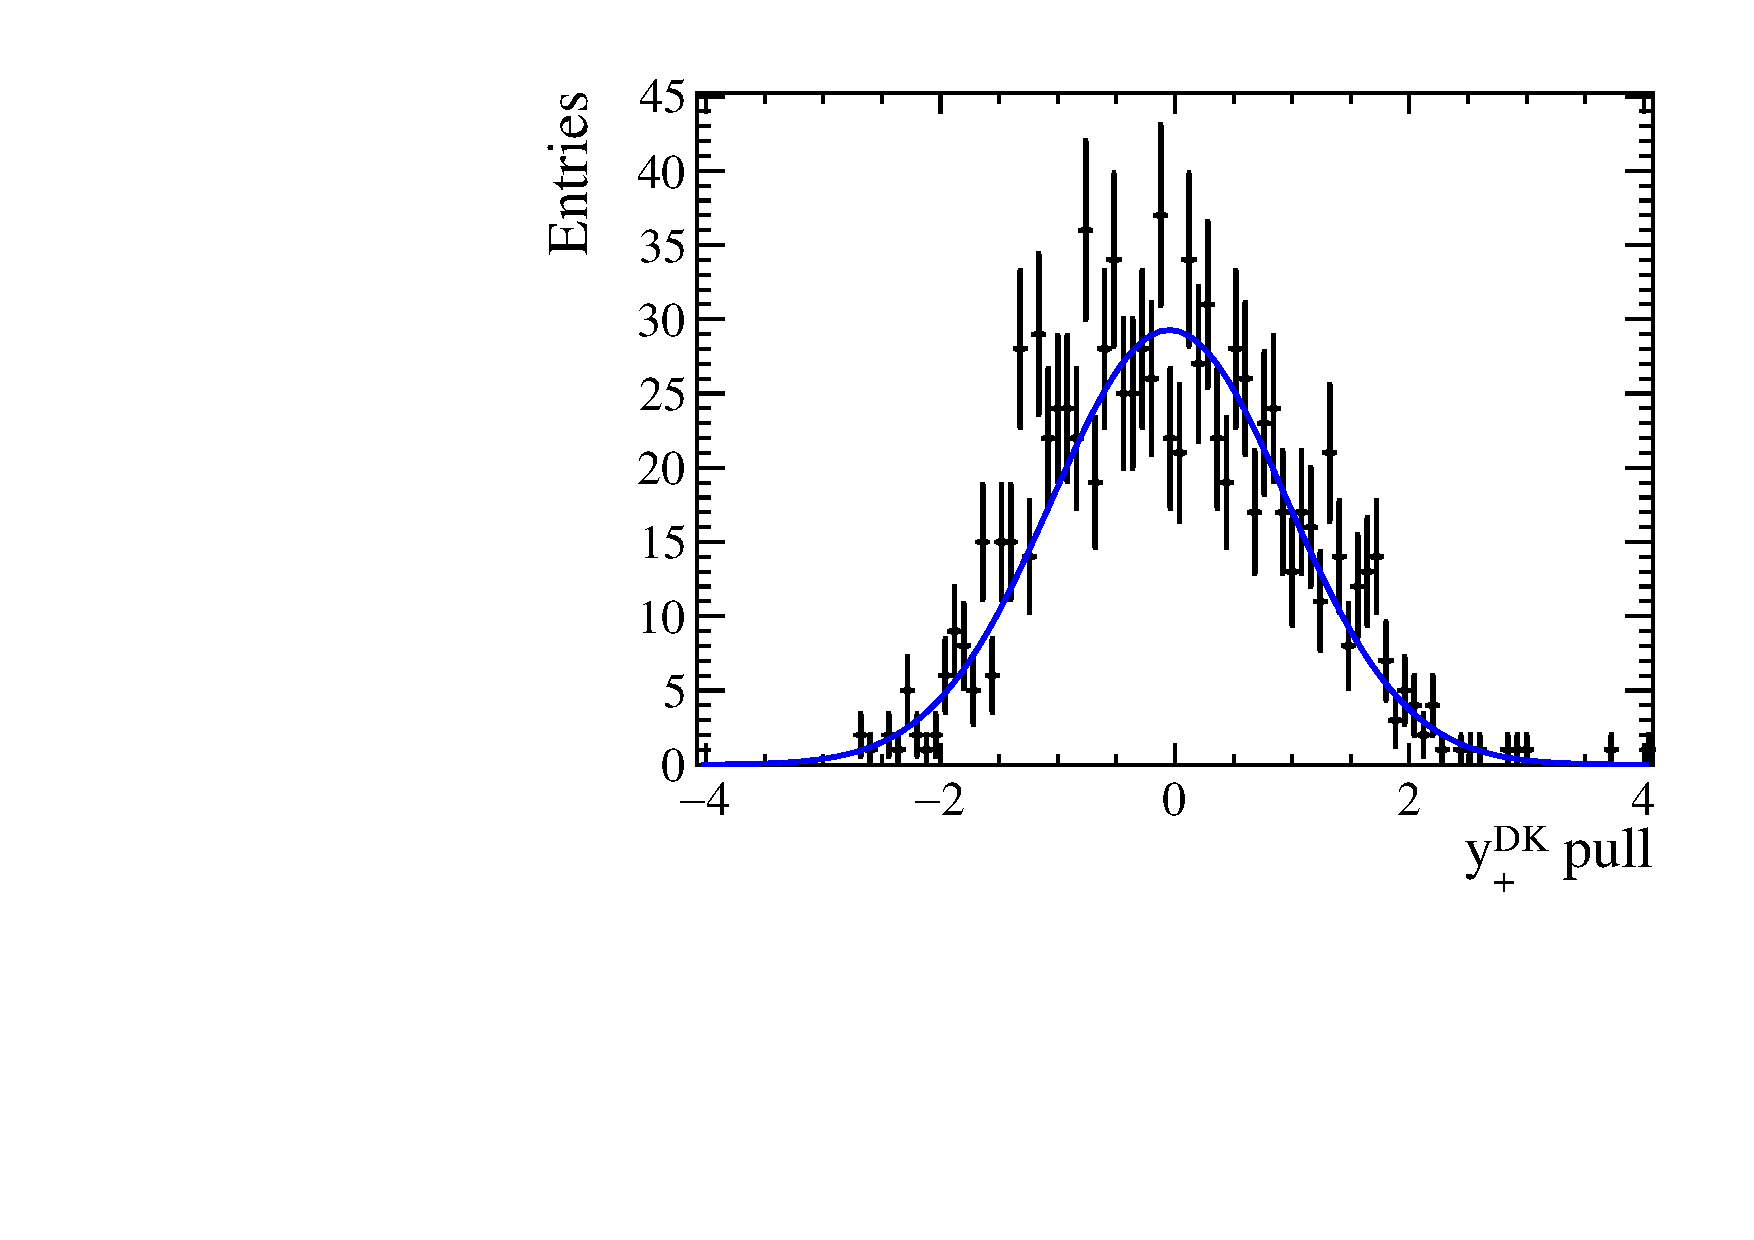
\includegraphics[width=1.0\textwidth]{Plots/A_yp_dk_pull.pdf}
      \vspace{-0.3cm}
      \caption*{$y_+^{DK}$}
    \end{subfigure}
    \caption*{$D^0\to K^+K^-\pi^+\pi^-$}
  \end{figure}
\end{frame}

\begin{frame}{Backup: Likelihood scan of CP observables}
  \begin{center}
    $x_\pm^{DK}$ agree well between likelihood scan and Hesse approximation
  \end{center}
  \begin{figure}
    \centering
    \begin{subfigure}{0.5\textwidth}
      \centering
      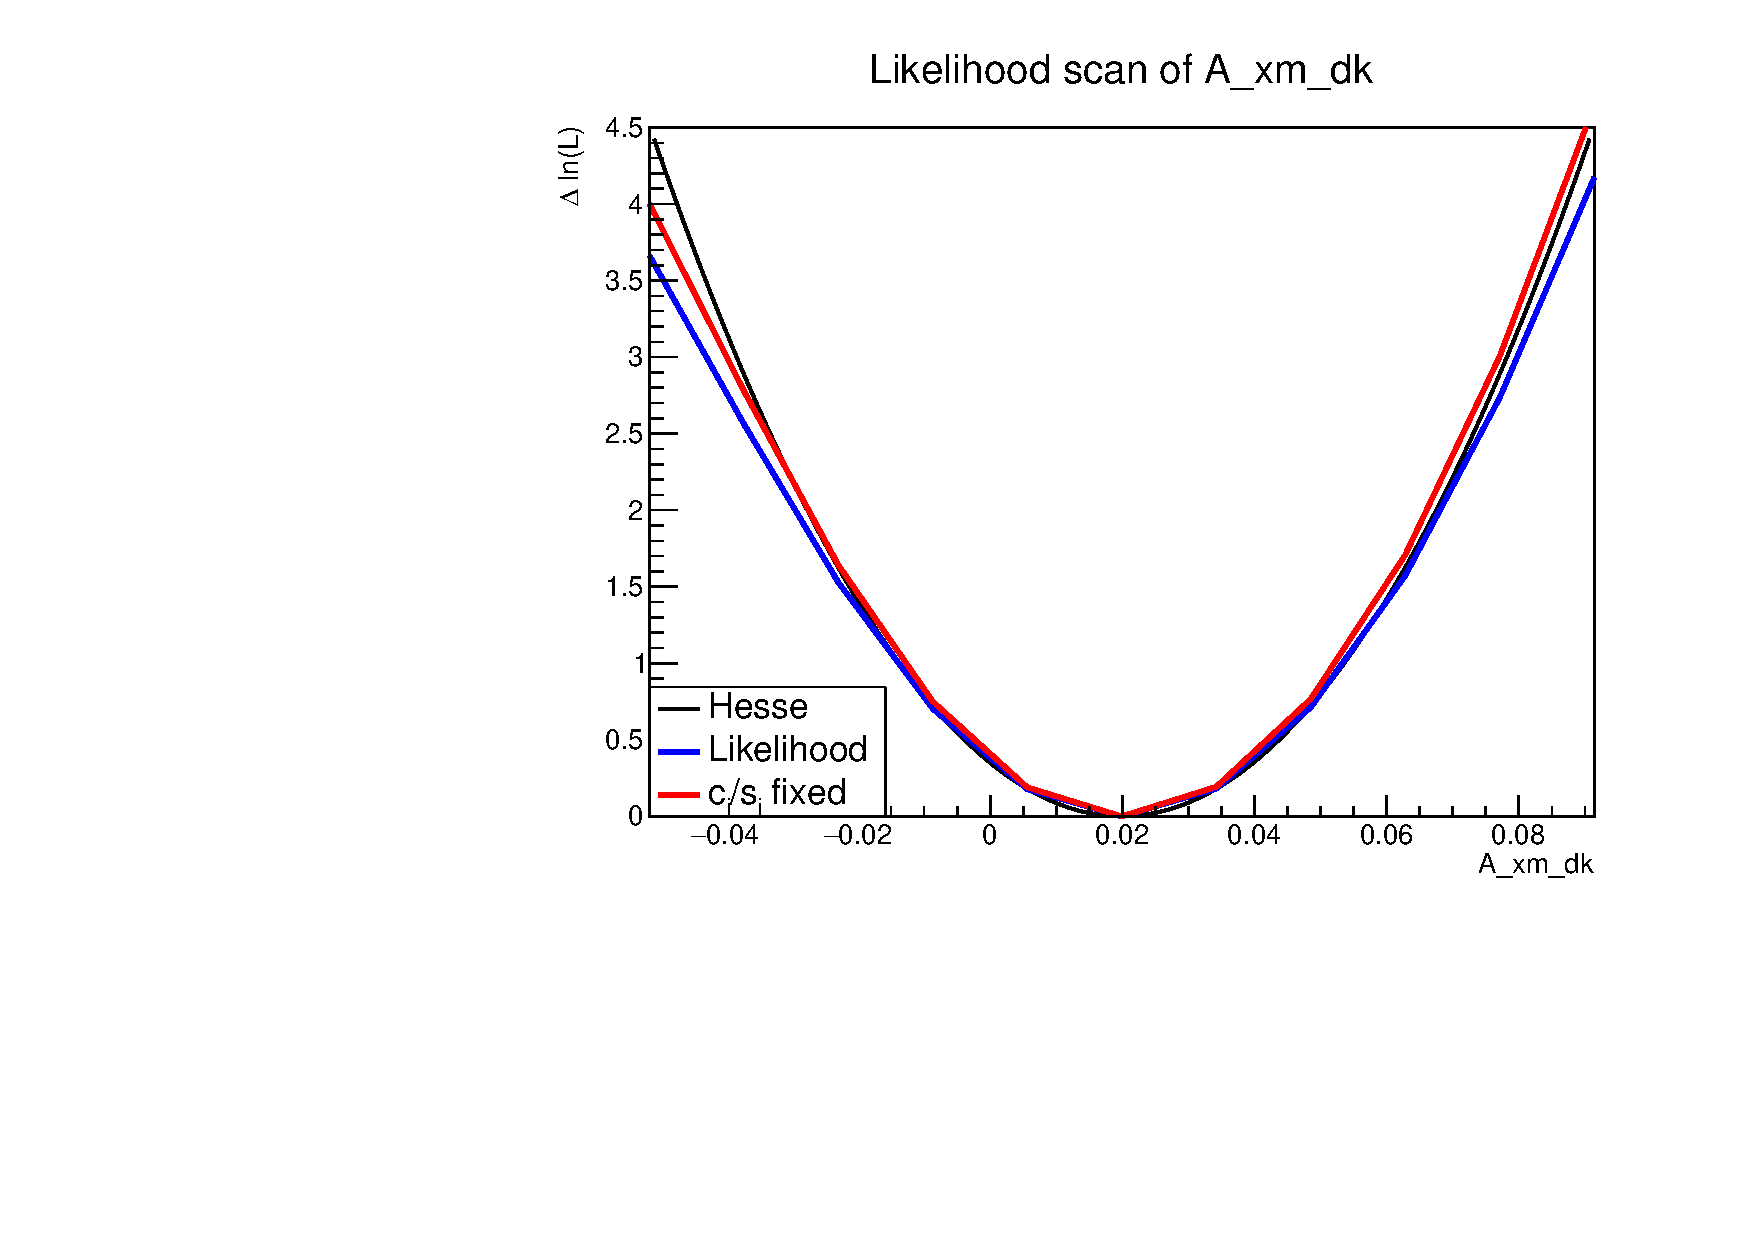
\includegraphics[width=1.0\textwidth]{Plots/A_xm_dk_likelihood_scan_pipipipi.pdf}
      \vspace{-0.3cm}
      \caption*{$x_-^{DK}$}
    \end{subfigure}%
    \begin{subfigure}{0.5\textwidth}
      \centering
      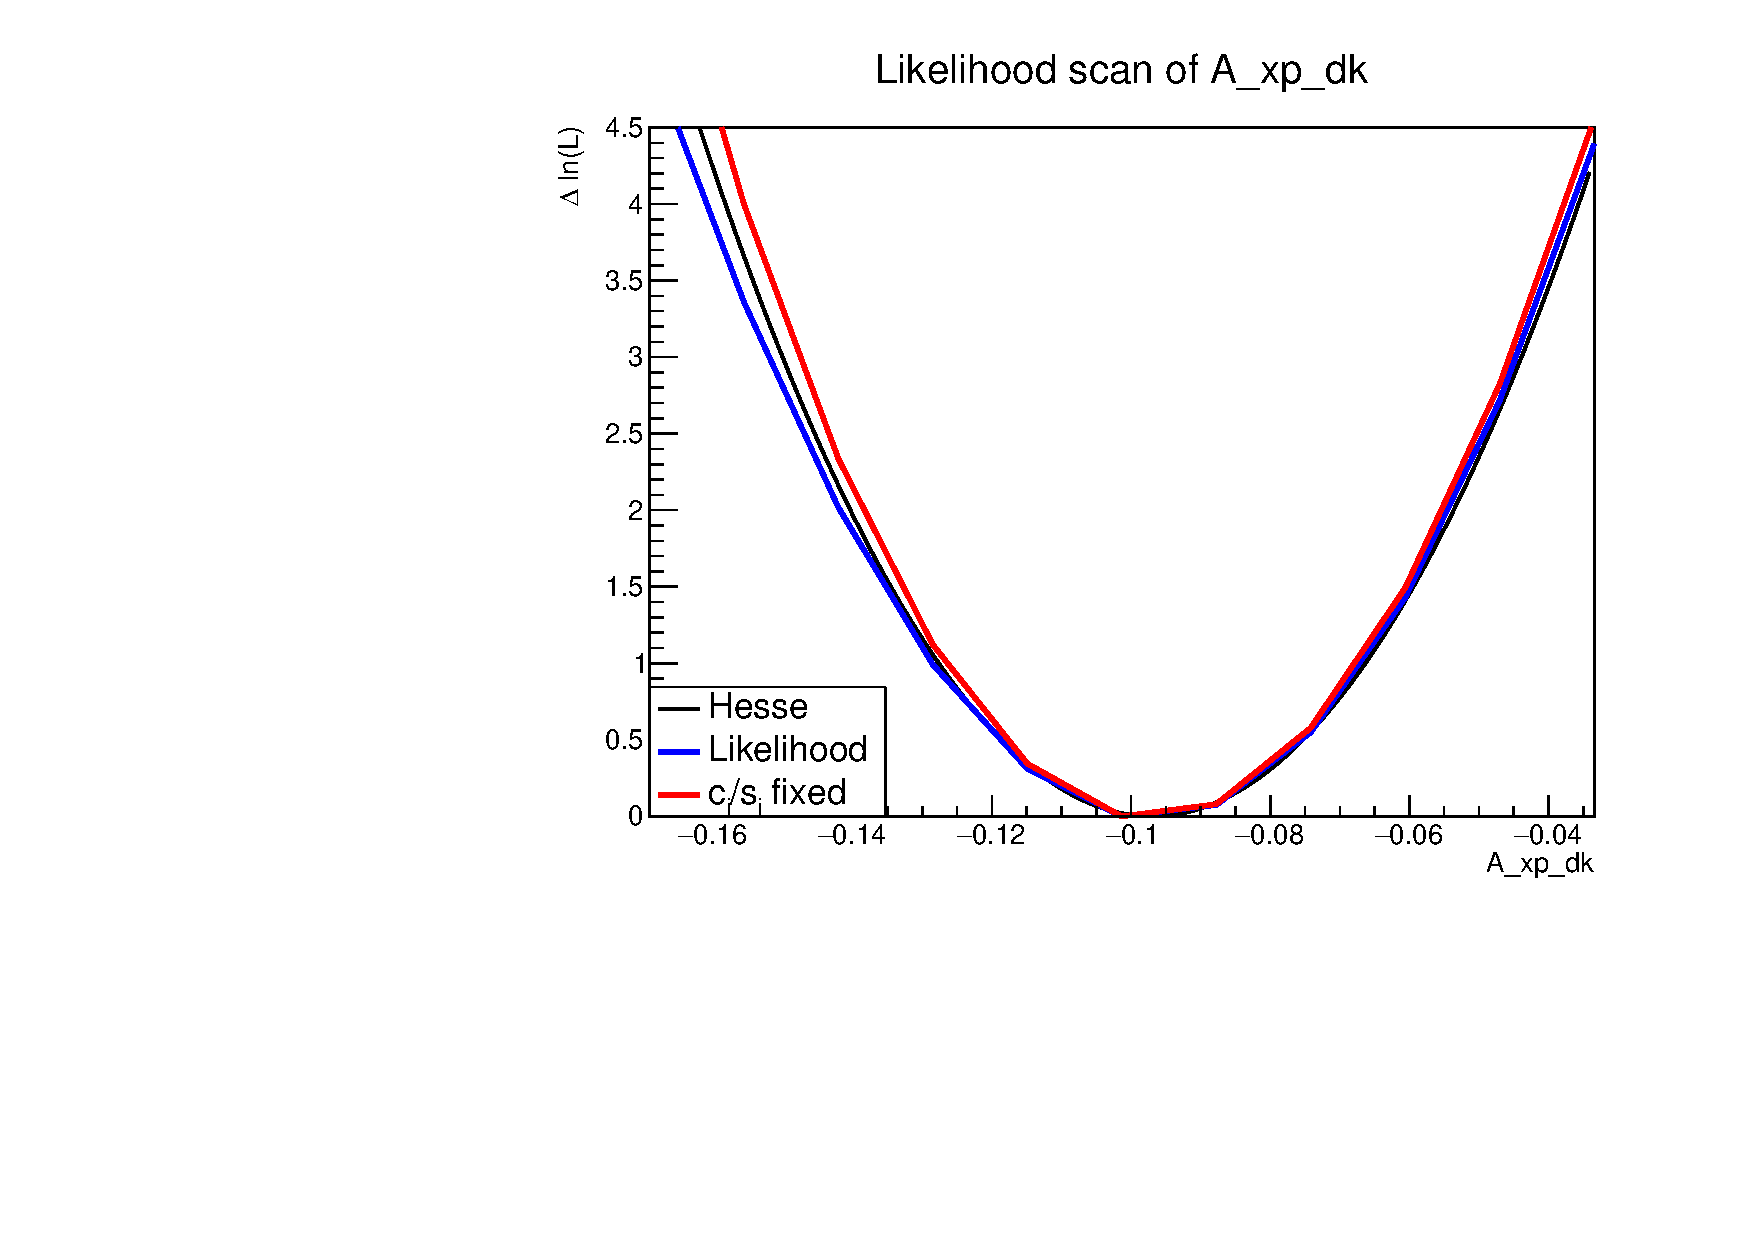
\includegraphics[width=1.0\textwidth]{Plots/A_xp_dk_likelihood_scan_pipipipi.pdf}
      \vspace{-0.3cm}
      \caption*{$x_+^{DK}$}
    \end{subfigure}
    \caption*{$D^0\to\pi^+\pi^-\pi^+\pi^-$}
  \end{figure}
\end{frame}

\begin{frame}{Backup: Likelihood scan of CP observables}
  \begin{center}
    $y_\pm^{DK}$ diverges from Hesse approximation outside $1\sigma$
  \end{center}
  \begin{figure}
    \centering
    \begin{subfigure}{0.5\textwidth}
      \centering
      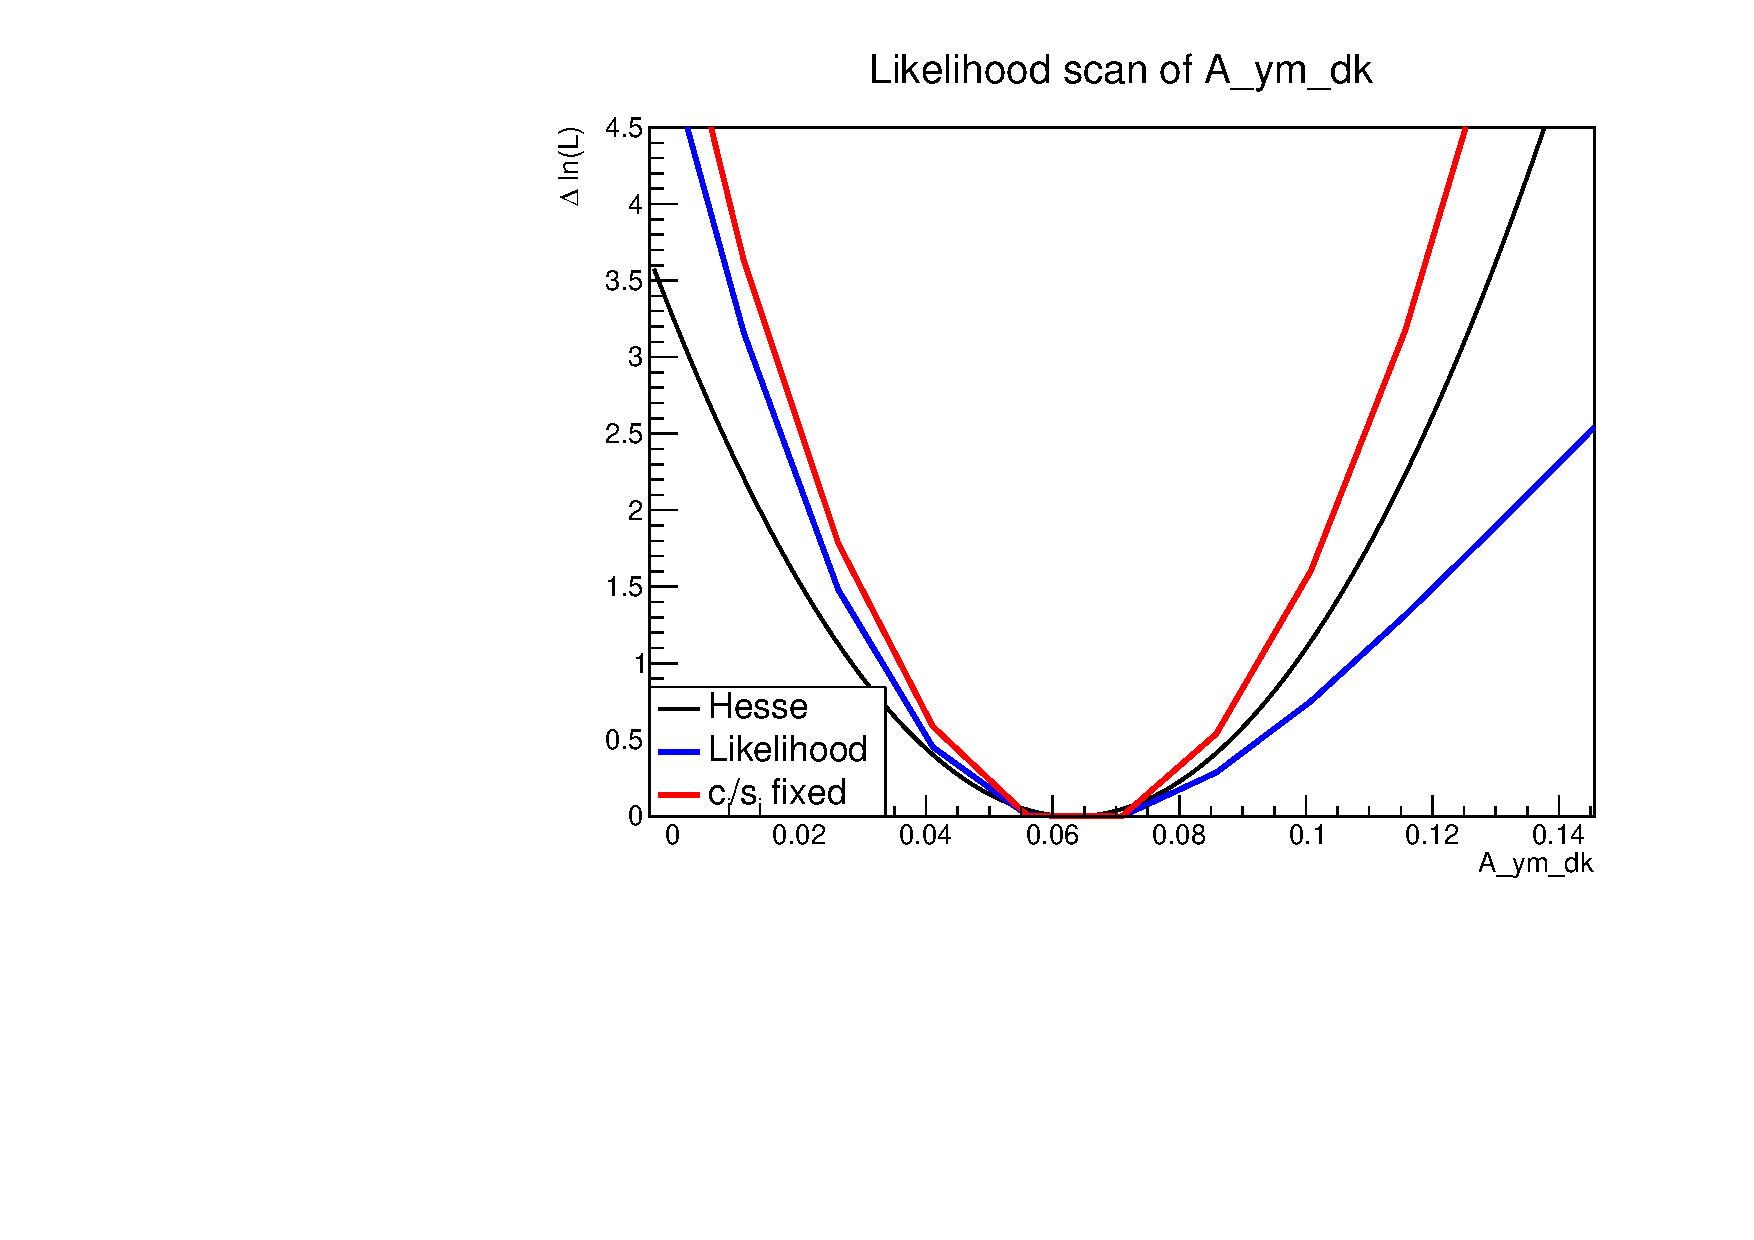
\includegraphics[width=1.0\textwidth]{Plots/A_ym_dk_likelihood_scan_pipipipi.pdf}
      \vspace{-0.3cm}
      \caption*{$y_-^{DK}$}
    \end{subfigure}%
    \begin{subfigure}{0.5\textwidth}
      \centering
      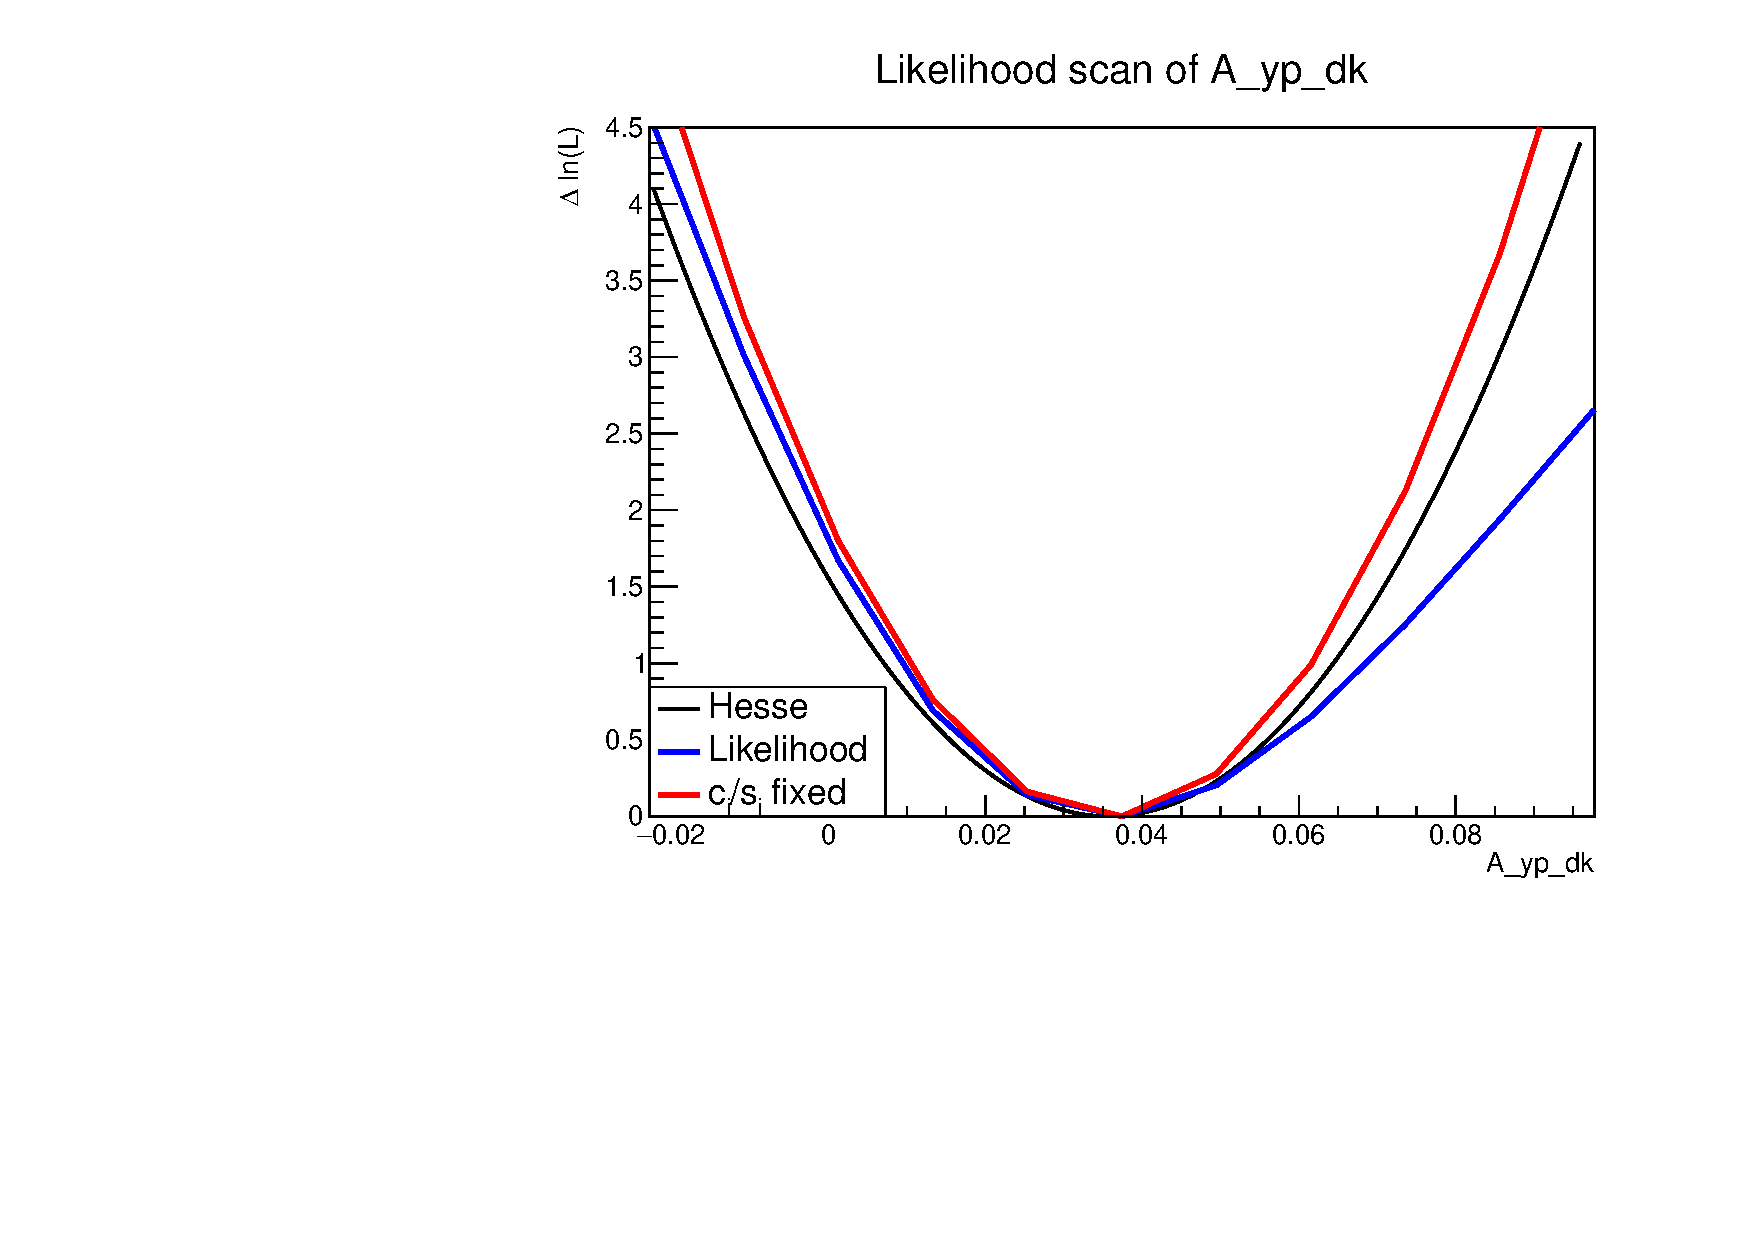
\includegraphics[width=1.0\textwidth]{Plots/A_yp_dk_likelihood_scan_pipipipi.pdf}
      \vspace{-0.3cm}
      \caption*{$y_+^{DK}$}
    \end{subfigure}
    \caption*{$D^0\to\pi^+\pi^-\pi^+\pi^-$}
  \end{figure}
\end{frame}

\begin{frame}{Backup: Interpretation toys}
  \begin{center}
    We can perform toy studies on the interpretation fit, but we do \underline{not} expect these to behave very Gaussian...
  \end{center}
  \begin{figure}
    \centering
    \begin{subfigure}{0.5\textwidth}
      \centering
      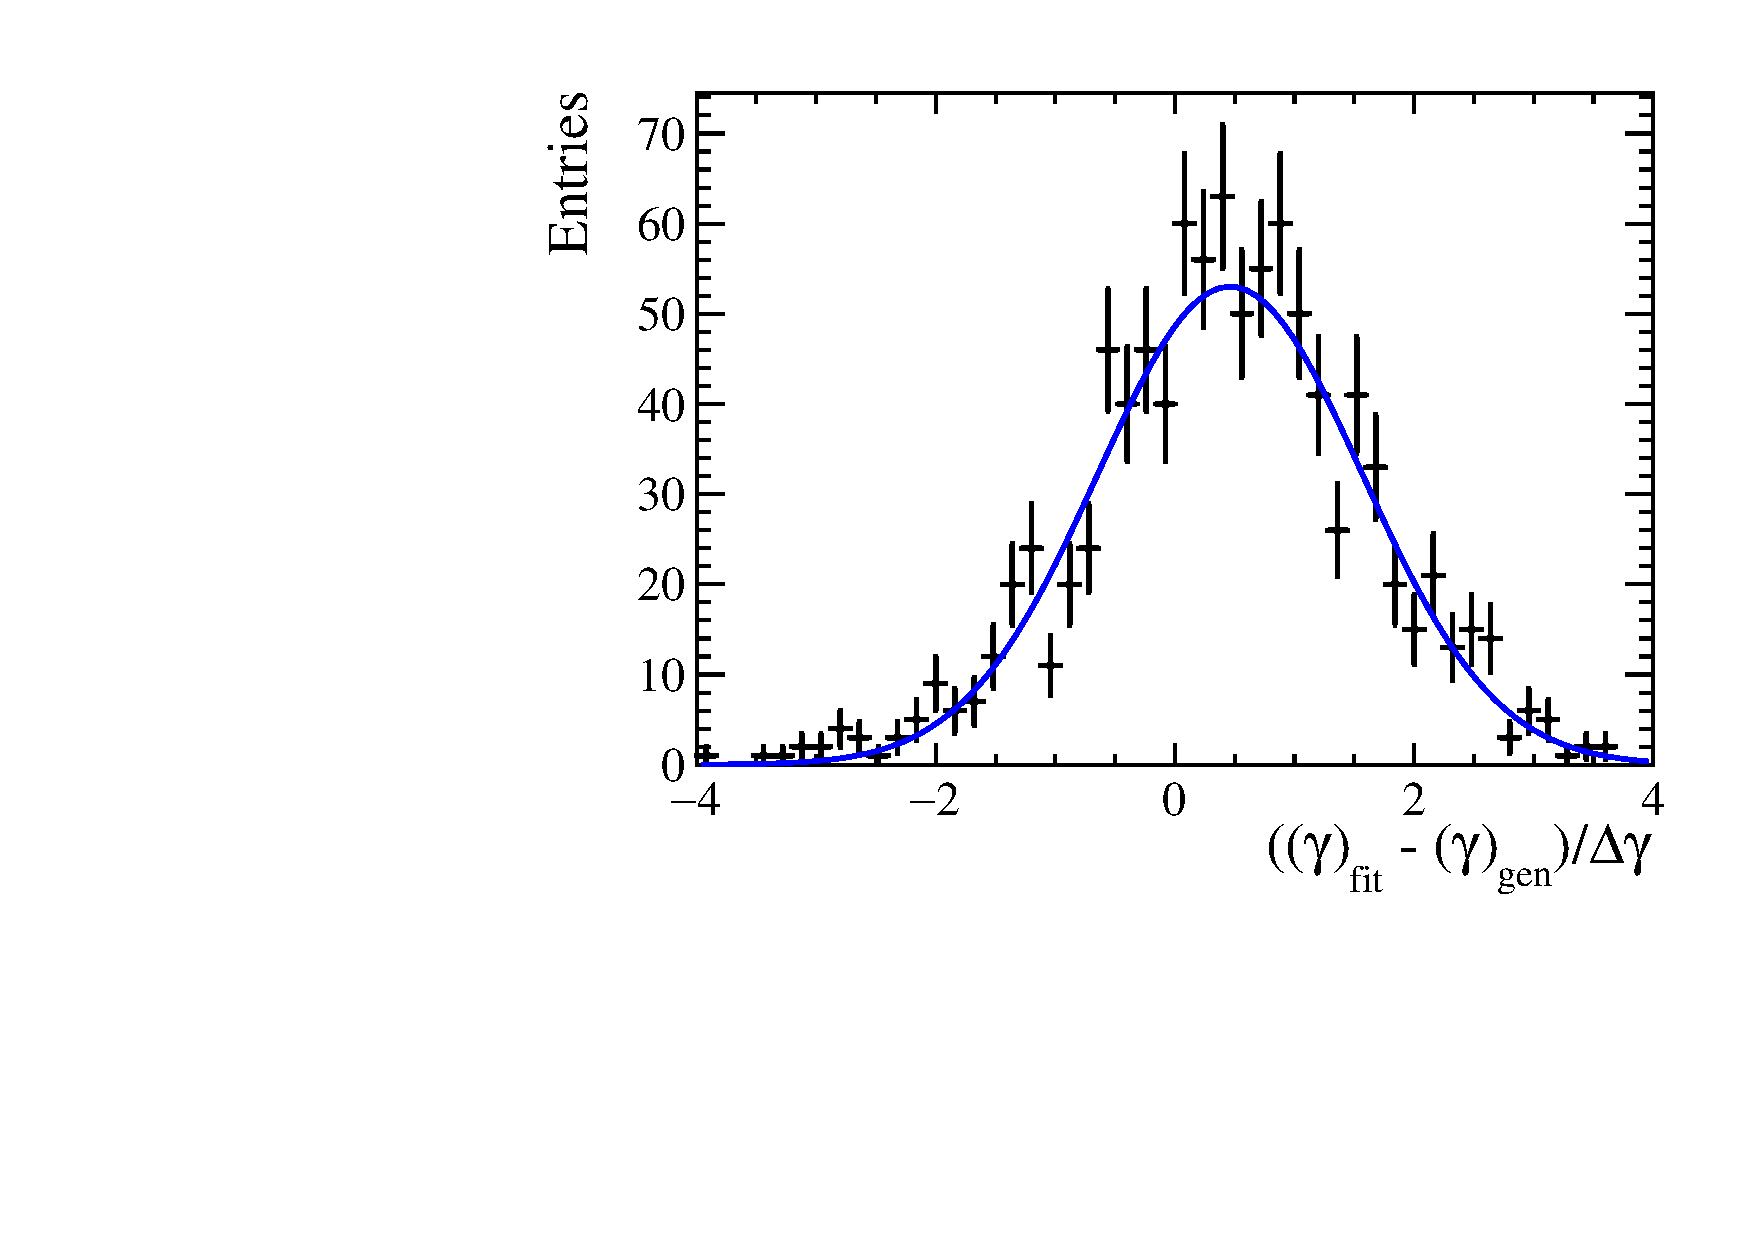
\includegraphics[width=1.0\textwidth]{Plots/gamma_pull_toys_KKpipi.pdf}
      \vspace{-0.3cm}
      \caption*{$K^+K^-\pi^+\pi^-$}
    \end{subfigure}%
    \begin{subfigure}{0.5\textwidth}
      \centering
      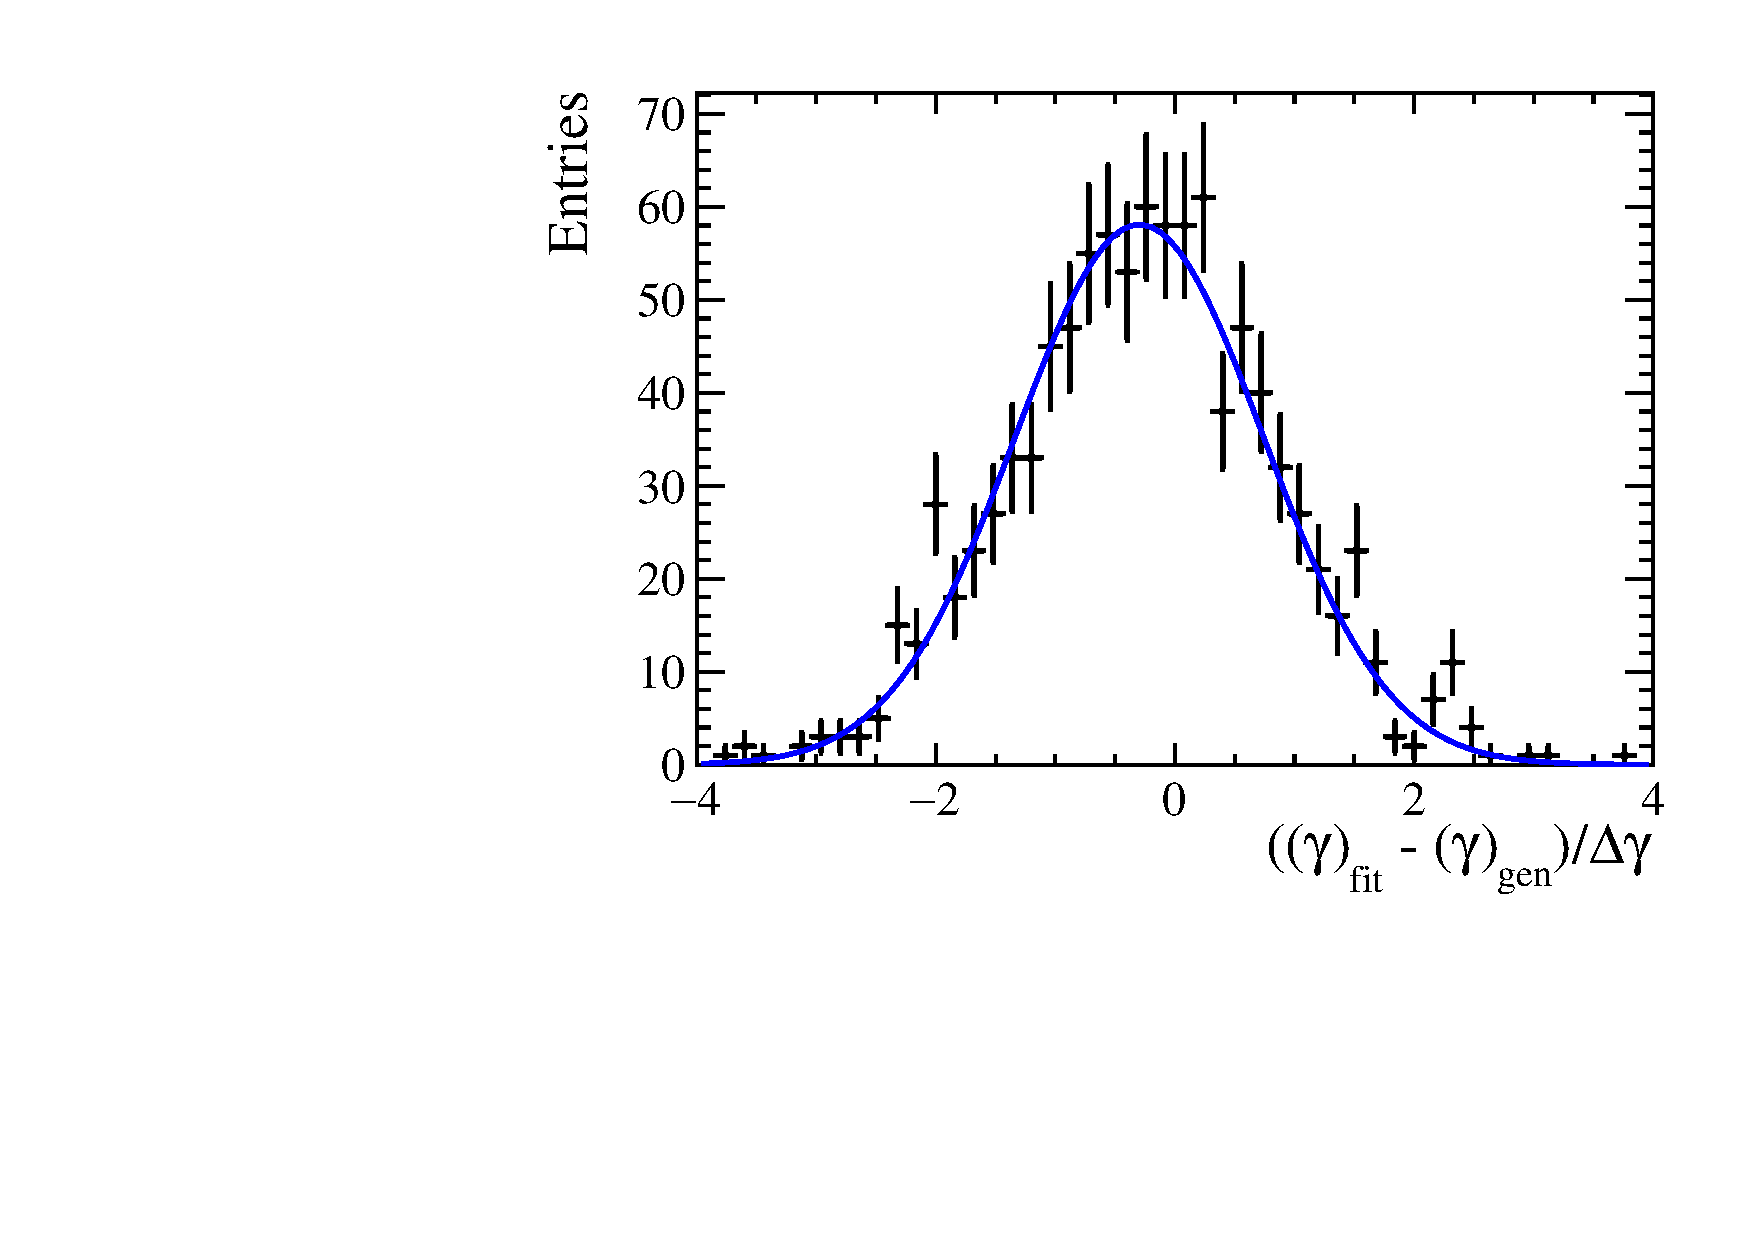
\includegraphics[width=1.0\textwidth]{Plots/gamma_pull_toys_pipipipi.pdf}
      \vspace{-0.3cm}
      \caption*{$\pi^+\pi^-\pi^+\pi^-$}
    \end{subfigure}
    \vspace{-0.5cm}
    \caption*{$\gamma$ pull distributions}
  \end{figure}
  \vspace{-0.3cm}
  \begin{center}
    Indeed, small but significant biases are observed!\\
    Use pull distributions to correct central values of physics parameters
  \end{center}
\end{frame}

\end{document}
